% ============================================================
% thesis_main.tex
% Networks of Influence: Legislative Text Diffusion in
% State Reproductive Policy After Dobbs
% Liliana Kowalski — UW-Madison Political Science
%
% CITATION STYLE: APSA Author-Date Parenthetical
%   In-text:       \parencite{key}        → (Author Year)
%                  \parencite[p.~12]{key} → (Author Year, p. 12)
%                  \textcite{key}         → Author (Year)
%   Discursive fn: \footnote{...}         → keep for substantive notes;
%                  use \parencite{} inside for any embedded citations
%   BANNED:        \footnote{\cite{key}}  → convert ALL to inline \parencite{}
%                  "see n. X" cross-refs  → replace with full \parencite{} repeated
% ============================================================
\listfiles  % put this before \documentclass
\documentclass[12pt]{report}
\usepackage{guthesis}

% CORE FORMATTING
% ============================================================

\setlength{\parindent}{0pt}
\setlength{\parskip}{0.5\baselineskip plus 2pt}

% Widow/orphan control
\widowpenalty=10000
\clubpenalty=10000
\raggedbottom

% ============================================================
% PACKAGES — each loaded exactly once
% ============================================================

% Mathematics
\usepackage{amsmath}
\usepackage{amssymb}

% Graphics and figures
\usepackage{graphicx}
\usepackage{subcaption}
\usepackage{float}
\graphicspath{{ch_findings/}}

% TikZ and plots
\usepackage{tikz}
\usetikzlibrary{positioning}
\usepackage{pgfplots}
\pgfplotsset{compat=1.18}

% Tables
\usepackage{booktabs}
\usepackage{tabularx}
\usepackage{threeparttable}
\usepackage{etoolbox}
\appto\TPTnoteSettings{\footnotesize}
\renewcommand{\TPTminimum}{0pt}
\usepackage{dcolumn}
\usepackage{array}
\usepackage{multirow}
\usepackage{lscape}
\usepackage{longtable}

% URLs
\usepackage{url}

% Typography and layout
\usepackage{parskip}
\usepackage{titlesec}

% Algorithms (retain if needed for computational methods chapter)
\usepackage{algorithm}
\usepackage{algorithmic}

% Footnote formatting: flush with margin, hanging indent
\usepackage[hang,flushmargin]{footmisc}
\setlength{\skip\footins}{1.5\baselineskip}
\addtolength{\footnotesep}{2pt}

% Section page breaks
\newcommand{\sectionbreak}{\clearpage}

% ============================================================
% BIBLIOGRAPHY — APSA AUTHOR-DATE (parenthetical)
% ============================================================
%
% biblatex with style=apa produces (Author Year) in-text citations,
% which satisfies APSA's author-date parenthetical requirement.
% Compile sequence: pdflatex → biber → pdflatex → pdflatex
%
% If your institution requires the 'apsr' .bst style instead,
% ============================================================
\usepackage[style=authoryear, backend=biber, uniquename=false]{biblatex}
\renewcommand*{\nameyeardelim}{\addspace}
\addbibresource{litreview.bib}

% Strip URLs, DOIs, access dates, and identifiers from all entries
\AtEveryBibitem{%
  \clearfield{url}%
  \clearfield{urldate}%
  \clearfield{doi}%
  \clearfield{isbn}%
  \clearfield{issn}%
  \clearfield{eprint}%
  \clearfield{eprinttype}%
}

\AtEveryCitekey{%
  \clearfield{url}%
  \clearfield{urldate}%
  \clearfield{doi}%
  \clearfield{isbn}%
  \clearfield{issn}%
  \clearfield{eprint}%
  \clearfield{eprinttype}%
}

% Suppress urldate field for online, report, and misc entry types
\DeclareFieldFormat[online]{urldate}{}
\DeclareFieldFormat[report]{urldate}{}
\DeclareFieldFormat[misc]{urldate}{}

% Legal citation driver (case names, statutes)
% Format: Title. Year.
\DeclareBibliographyDriver{legal}{%
  \printfield{title}%
  \newunit\newblock
  \printfield{year}%
  \finentry
}

% ============================================================
% THEOREM / PROOF ENVIRONMENTS (retain for methods appendix)
% ============================================================

\newtheorem{theorem}{Theorem}[section]
\newenvironment{proof}[0]{\textit{Proof.}}{}
\newcommand{\qed}{\hfill $\Box$}
\newcolumntype{Y}{>{\raggedright\arraybackslash}X}

% Comment-out macro
\long\def\comment#1{}

% ============================================================
% UW-MADISON THESIS PACKAGE
% ============================================================
% ============================================================
% TITLE PAGE METADATA
% ============================================================

\title{Networks of Influence: Legislative Text Diffusion in State Reproductive Policy After Dobbs}
\author{Liliana Kowalski}
\previousdegree{B.A., Political Science}
\thisdiscipline{Political Science}
\thesistype{Thesis}
\thesismonth{May}
\thesisyear{2026}
\newcommand{\guthesisday}{9}
\professor{Eleanor Neff Powell}
\fulltitle{Networks of Influence: Legislative Text Diffusion in State Reproductive Policy After \textit{Dobbs}}
\indexwords{policy diffusion, post-\textit{Dobbs} abortion policy, state legislatures, computational text analysis, legislative templating, advocacy coalitions,
constitutional vacuum diffusion, dyadic regression, TF-IDF cosine similarity,
reactive template mobilization}

% CHAPTERS
%
% NOTE ON CONVERTING CHAPTER FILES:
% In chapter2_litreview.tex, chapter3_methodology.tex, etc., replace:
%   \footnote{\cite{key}}                → \parencite{key}
%   \footnote{\cite{key}, p. X}          → \parencite[p.~X]{key}
%   Author (Year)\footnote{\cite{key}}   → \textcite{key}
%   "see n. X" or "see fn. X"           → \parencite{key}  (full citation repeated)
% Retain \footnote{} ONLY for substantive discursive content.
% Embedded citations within discursive footnotes use \parencite{} inside the \footnote{}.

\begin{document}

\maketitle

\begin{abstract}
This thesis examines how abortion-related legislation diffused across U.S. states in the first full legislative year after \textcite{DobbsJacksonWomens2021}. Drawing on a corpus of 188 enacted bills across 46 states, it uses computational text analysis---TF--IDF cosine similarity computed across 104{,}445 unique n-grams---together with bill-level and dyadic regression to identify the structural predictors of textual convergence. Three findings invert conventional expectations. First, protective coalitions, not restrictive ones, deployed standardized legislative templates most aggressively in 2023: protective bills are significantly less novel than neutral bills ($\beta = -0.076$, $p = 0.022$), while restrictive bills are statistically indistinguishable from the neutral baseline. Second, the highest textual convergence across state lines coexists with a near-complete absence of direct PAC contributions between coordinated legislators, indicating that diffusion operates through informational rather than financial channels. Third, at the state-pair level, shared advocacy organization co-presence (PAC Jaccard $\beta = +0.039$, $p < 0.001$) and shared protective coalition membership ($\beta = +0.037$, $p < 0.001$) predict textual similarity while geographic contiguity is null ($\beta = +0.003$, $p = 0.734$). The thesis advances a framework of \emph{constitutional vacuum diffusion}, with \emph{reactive template mobilization} as its operative mechanism, and distinguishes vertical (restrictive) from horizontal (protective) coalition architectures in their production of detectable textual signatures.
\end{abstract}

\begin{center}
\pseudochapter{Acknowledgments}
I would like to extend my deepest gratitude to my advisor, Professor Eleanor Neff Powell, for her guidance and mentorship throughout this project. To Professor Amy Gangl and my fellow thesis writers, for their wisdom and feedback week after week. And to my family, my partner, and the
friendships I have made along the way---for every late-night conversation
and every message of support.

None of this would have been possible without you.
\end{center}

\tableofcontents
\listoffigures
\listoftables

% Chapter 1 — Introduction
\chapter{Introduction}
\label{ch:introduction}

\section{The Puzzle of Post-\textit{Dobbs} Diffusion}

On June 24, 2022, the Supreme Court issued its decision in \textit{Dobbs v. Jackson Women's Health Organization}, overruling \textcite{RoeWade1971} and \textcite{PlannedParenthoodSoutheastern1992} and returning the regulation of abortion to the states. The decision did not merely alter constitutional doctrine. It collapsed, in a single opinion, the federal preemption regime that had structured state-level reproductive policy for nearly half a century. The states became, overnight, the exclusive jurisdictional venue for a contested policy domain in which both regulatory expansion and codification of protections had been institutionally constrained for two generations.

The legislative response was rapid, substantively bilateral, and---I will argue---structurally novel. By the close of the 2023 legislative session, forty-six states had enacted at least one statute responsive to the new constitutional environment, producing a corpus of 188 bills that ranged from six-week gestational limits and trigger statutes to shield laws, codified clinic protections, and procedural expansions of access. The textual record of that single legislative year is the empirical object I analyze.

The accumulated literature on policy diffusion did not anticipate the characteristic features of this record. The geographic-learning tradition, descending from \textcite{walkerDiffusionInnovationsAmerican1969}, predicts that innovation spreads through regional clusters as adopting states observe and adapt to the experience of nearby pioneers. The event-history framework of \textcite{berryStateLotteryAdoptions1990} specifies internal determinants and regional influence as the principal predictors of adoption timing. The copy-and-paste tradition formalized by \textcite{jansaCopyPasteLawmaking2019} predicts that interest-group drafting infrastructure produces detectable textual signatures, and---given the institutional prominence of national restrictive-coalition organizations in pre-\textit{Dobbs} abortion policy---should produce its strongest signature on the restrictive side. None of these predictions accurately describe the 2023 record. Geographic contiguity is statistically null as a predictor of cross-state textual similarity. Coalition coordination is detectable, but it is concentrated on the protective rather than the restrictive side. And the diffusion timeline is too compressed for the observational learning the geographic tradition presupposes: bills enacted in March cannot be the product of states having watched the consequences of bills enacted in February.

The empirical puzzle, then, concerns diffusion regimes. When federal preemption abruptly collapses in a highly salient, organizationally mature policy domain, what mechanism replaces the slow regional learning the field has theorized? The answer I develop is that the mechanism is not learning at all. It is the activation of pre-positioned templates through coalition-aligned organizational networks---a regime that the diffusion literature has not previously needed to specify, and one whose signatures are visible in the textual record of the first post-shock legislative cycle.

\section{The Argument}

I advance four interlocking claims. The first is empirical: the 2023 post-\textit{Dobbs} abortion corpus exhibits a characteristic textual structure---moderate cross-state borrowing rather than either wholesale copying or independent drafting, with two-thirds of bills clustered between 0.70 and 0.90 on the cross-state novelty measure---and that structure is coalition-asymmetric. Protective bills are significantly less novel than the neutral baseline ($\beta = -0.076$, $p = 0.022$); restrictive bills are not statistically distinguishable from it ($\beta = -0.017$, $p = 0.482$). At the dyadic level, cross-state textual similarity is predicted by shared organizational infrastructure ($\beta = +0.039$, $p < 0.001$, measured as the Jaccard index of PAC donor organizations) and by shared protective coalition membership ($\beta = +0.037$, $p < 0.001$), not by geographic contiguity ($\beta = +0.003$, $p = 0.734$). These findings invert the pre-\textit{Dobbs} expectation that restrictive-coalition templating would dominate the observable record.

The second claim is theoretical. The thesis develops a framework---\emph{constitutional vacuum diffusion}---that specifies the structural conditions under which the empirical signature documented here should be expected: a judicially imposed rather than discursively negotiated policy window, a bilateral rather than unilateral opportunity structure, a compressed temporal horizon, and a pre-existing advocacy infrastructure that positioned model language before the precipitating shock. Within that framework, the thesis identifies \emph{reactive template mobilization} as the operating mechanism: pre-built statutory language, refined over years by organizations on both sides of the issue, is activated through affiliate channels in the months immediately following the shock. The mechanism is distinct from learning-based diffusion (which presupposes time to observe consequences), from conventional crisis adoption (which presupposes templates produced in response to the precipitating event), and from the Shipan and Volden four-mechanism typology (whose categories the post-shock hybrid does not cleanly match).

The third claim concerns coalition architecture. The asymmetry between restrictive and protective coordination is not, on the evidence assembled here, an accident of mobilization timing. It reflects two distinct organizational forms: a vertical architecture on the restrictive side, in which template development concentrates within a small number of national nodes (Americans United for Life, Susan B. Anthony Pro-Life America, the Alliance Defending Freedom) that distribute language outward to allied state legislators; and a horizontal architecture on the protective side, in which state-level affiliates of the principal advocacy organizations (Planned Parenthood, the ACLU, the Center for Reproductive Rights, Reproductive Freedom for All (RFA)) coordinate laterally on a shared codification agenda. These architectures produce different textual signatures, and the 2023 record is consistent with both operating simultaneously.

The fourth claim is methodological. The dissociation between financial transfer and textual coordination---reported across the ten highest-similarity bill pairs and confirmed by systematic analysis of the DIME contribution record---provides empirical support for the \textcite{hallLobbyingLegislativeSubsidy2006a} legislative-subsidy framework in a policy domain where the financial-influence intuition has been particularly prominent in public commentary. The organizations whose Jaccard overlap predicts convergence are not purchasing legislative behavior. They are supplying informational infrastructure: model language, legal memoranda, drafting assistance, and expert testimony. Contribution-only measures of interest-group influence systematically misspecify the channel through which coordination operates in this domain.

\section{Scope, Approach, and Limits}

This thesis was designed to answer a narrow question with precision: what textual and structural patterns characterize cross-state diffusion in the first post-\textit{Dobbs} legislative cycle, and which institutional and coalitional features predict them? The empirical scope is correspondingly constrained. The analysis covers a single legislative year (2023), a single policy domain (abortion regulation), and a single national context (the United States). It analyzes enacted legislation rather than the full population of introduced bills. It measures textual similarity through TF--IDF cosine distance over $n$-gram representations rather than through semantic embeddings. And it operationalizes organizational infrastructure through PAC donor co-presence rather than through richer measures of organizational depth that would require lobby-disclosure and IRS data, the thesis does not incorporate.

These choices were deliberate prioritizations rather than concessions, a framing developed at length in Section~\ref{sec:designed-scope}. The single-year scope isolates the initial legislative response to the constitutional shock before feedback effects from judicial challenges and electoral consequences could contaminate the diffusion signal. The enacted-bill scope captures the completed output of the legislative process and avoids the interpretive ambiguity of bills whose failure may reflect strategic withdrawal rather than substantive rejection. The TF--IDF representation provides transparent, reproducible textual measurement consistent with the broader text-as-data literature on legislative similarity \parencite{wilkersonTracingFlowPolicy2015,linderTextPolicyMeasuring2020}. Each choice carries inferential costs, and Chapter~\ref{ch:limitations} specifies them explicitly along with the future research agenda---qualitative inquiry into drafting processes, archival enrichment of organizational measures, longitudinal corpus extension, cross-domain replication, and semantic methodological refinement---that would address them.

The argument's implication structure extends well beyond the narrow empirical question. If constitutional vacuum diffusion is a generalizable regime rather than a description of one policy area's idiosyncratic post-shock dynamics, the framework should travel to other domains in which federal doctrinal infrastructure has collapsed or may collapse---firearms regulation following \textit{New York State Rifle \& Pistol Association v. Bruen}, voting rights following \textit{Shelby County v. Holder}, hypothetical reversals of other long-standing constitutional doctrines. Whether the framework does travel is an empirical question that the present thesis raises but does not answer. The contribution it makes is to specify the framework precisely enough that subsequent research can evaluate it.

\section{Plan of the Thesis}

The chapters that follow proceed from the literatures the thesis draws on through the empirical analysis to the theoretical apparatus and its limits.

Chapter~\ref{ch:theory} reviews the diffusion literature that the thesis engages and revises: the geographic tradition, the event-history framework, the copy-and-paste research program, the state-capture literature on organizational influence, and the four-mechanism typology of Shipan and Volden. It identifies the specific predictions each tradition generates for the post-\textit{Dobbs} environment and locates the analytical gap that constitutional vacuum diffusion is positioned to fill.

Chapter~\ref{ch:methodology} specifies the research design. It documents corpus construction from LegiScan records, the TF--IDF representation and cosine-similarity computation, the construction of the cross-state novelty measure, the bill-level regression specification, and the dyadic regression specification incorporating the PAC Jaccard organizational measure derived from the DIME database. It justifies the analytical choices the design makes and previews the limitations the design imposes.

Chapter~\ref{ch:findings} reports the empirical findings. It documents the distributional properties of the novelty measure, the bill-level regression results including the partial inversion of \textcite{squireMeasuringStateLegislative2007} on professionalism, and the dyadic regression results that establish organizational co-presence and coalition alignment as the structural predictors of cross-state textual similarity. It presents the case-level evidence of the Nevada SB 370--Washington HB 1155 near-replication and the dissociation between financial transfer and textual coordination across the highest-similarity bill pairs.

Chapter~\ref{ch:discussion} develops the theoretical apparatus. It introduces constitutional vacuum diffusion as a regime characterized by specific structural conditions, specifies reactive template mobilization as the operating mechanism within that regime, develops the vertical--horizontal coalition architecture distinction between restrictive and protective coordination, reinterprets the professionalism finding as a measure of capacity for adoption rather than capacity for innovation, and reconstructs the exporter--importer--reinforcer typology to accommodate the 2023 record's coalition-asymmetric structure.

Chapter~\ref{ch:limitations} specifies the limits of the design. It identifies the inferential gap between the textual signatures the analysis detects, and the mechanism-level claims the framework advances, articulates the rival mechanisms the design cannot eliminate, and develops the future research agenda---qualitative drafting-process inquiry, archival enrichment, longitudinal extension, cross-domain replication, and semantic methodological refinement---that subsequent investigation should pursue.

Chapter~7 consolidates the contributions, locates the thesis within the trajectory of diffusion scholarship, and closes with the interpretive question the 2023 record poses most urgently for the field: whether the patterns documented here represent a transitional anomaly of the immediate post-\textit{Dobbs} mobilization period or the first evidence of a structural transformation in how American states make policy after constitutional shocks. That question cannot be resolved from a single legislative year. The analytical infrastructure assembled here is designed to support its resolution by the research that follows.

% Chapter 2 — Theoretical Frameworks
% CHAPTER 2: THEORETICAL FRAMEWORKS

\chapter{Theoretical Frameworks}
\label{ch:theory}

\section{Introduction}

On June 24, 2022, the Supreme Court's decision in \textit{Dobbs} v. \textit{Jackson Women's Health Organization} removed the federal constitutional right to abortion that had existed since \textit{Roe} v. \textit{Wade} in 1973. The decision handed abortion policy back to the states, creating what I call a "constitutional vacuum"---a sudden absence of federal rules governing a highly contested policy area.

What followed presents a theoretical puzzle. If classic frameworks are correct, states should have adopted abortion policies gradually, learning from early adopters and adapting legislation to local contexts. If, alternatively, advocacy organizations had prepared legislative templates in anticipation of the decision, we might observe rapid, coordinated adoption with high textual similarity across states. Chapter~4 evaluates which scenario the empirical record more closely supports. Where foundational models predict gradual geographic spread over years or decades \parencite{walkerDiffusionInnovationsAmerican1969, berryStateLotteryAdoptions1990}, with higher-capacity states adopting first and lower-capacity states following \parencite{shipanMechanismsPolicyDiffusion2008a}, post-\emph{Dobbs} legislative activity suggests a fundamentally different temporal and spatial dynamic---one characterized by compressed timeframes, ideological rather than geographic clustering, and elevated textual coordination consistent with organizational template deployment.

\subsection{Three Puzzles}

Three specific puzzles, each emerging from tensions within the theoretical traditions reviewed below, motivate this research.

Throughout this thesis, I distinguish between two broad coalitions that mobilized following \emph{Dobbs}. The \emph{restrictive coalition} encompasses organizations, legislators, and advocacy networks working to limit or prohibit abortion access---including Americans United for Life, Alliance Defending Freedom, National Right to Life Committee, and their state-level affiliates. The \emph{protective coalition} encompasses those working to preserve or expand abortion access---including Planned Parenthood affiliates, the ACLU Reproductive Freedom Project, the Center for Reproductive Rights, and Reproductive Freedom for All (formerly NARAL Pro-Choice America). These labels---restrictive and protective---are used throughout as analytically neutral terms describing policy direction rather than normative orientation. Both coalitions are internally heterogeneous, with member organizations differing in strategy, emphasis, and institutional form, but the coalition-level distinction captures the fundamental organizational divide structuring post-\emph{Dobbs} legislative activity.

\paragraph{Puzzle 1: Why do restrictive and protective coalitions exhibit different coordination structures?}

Scholarship on policy entrepreneurship documents multiple coordination strategies available to advocacy coalitions \parencite{mintromPolicyEntrepreneurshipPolicy2009}, and organizational influence theory predicts that centralized template networks should produce different diffusion signatures than decentralized horizontal coordination \parencite{garrettInterestGroupInfluence2015,hertel-fernandezStateCapture2019}. Whether opposing coalitions within the same policy domain employ structurally different organizational architectures, and what observable textual patterns such differences would produce, remains an open empirical question.

\paragraph{Puzzle 2: How does policy coordination occur when financial pathways are absent?}

Campaign finance scholarship emphasizes the role of PAC contributions and lobbying expenditures in shaping legislative behavior \parencite{hallBuyingTimeMoneyed,baumgartner_jones_1993}. When major policy windows open, existing theory predicts substantial financial investment in newly salient arenas. Yet, organizational influence can also operate through informational mechanisms that require no financial transfer: legislative subsidies in the form of model bills, policy briefs, and expert testimony \parencite{hallLobbyingLegislativeSubsidy2006a}. Whether financial or informational mechanisms predominate in post-\emph{Dobbs} coordination is an open empirical question with implications for how we understand organized influence in American state politics.

\paragraph{Puzzle 3: What explains the speed and breadth of post-\emph{Dobbs} policy diffusion?}

Classic diffusion models describe a gradual process in which states learn from early adopters over years or decades, with adoption waves spreading through geographic or institutional networks \parencite{walkerDiffusionInnovationsAmerican1969,berryStateLotteryAdoptions1990,shipanMechanismsPolicyDiffusion2008a}. Punctuated equilibrium theory predicts rapid change following focusing events, but typically within individual jurisdictions rather than simultaneously across many \parencite{baumgartner_jones_1993}. \emph{Dobbs} created conditions that neither framework was designed to explain: a simultaneous policy opening across all fifty states, with pre-positioned organizational infrastructure ready to fill the regulatory space. Whether the resulting legislative activity follows patterns explicable by existing frameworks, or whether it requires theoretical extension, is a central question the empirical chapters investigate.

\subsection{Why Existing Theories Fall Short}

There is no singular theoretical framework that sufficiently explains the post-\textit{Dobbs} pattern. Classic diffusion theory explains gradual learning but not rapid coordination. Constitutional shock theories explain abrupt change but not pre-prepared deployment. Organizational influence theories explain template provision but not why different coalitions chose divergent strategies.

Text-as-data methods offer a powerful toolkit for systematic analysis of legislative language at scale. By converting bill texts into numerical representations through TF-IDF vectorization and computing pairwise similarity through cosine distance, researchers can identify patterns of textual convergence across hundreds of bills that would be impossible to detect through manual comparison alone \parencite{wilkersonTracingFlowPolicy2015,linderTextPolicyMeasuring2020}. These methods enable researchers to move beyond binary adoption measures---did a state enact a policy or not?---to continuous measures of \textit{how closely} states' legislative language converges, capturing gradations of borrowing, adaptation, and independent drafting that adoption-only frameworks miss \parencite{boehmkeStatePolicyInnovativeness2012a}.

However, computational text similarity is a necessary but insufficient indicator of policy diffusion. Text-as-data methods can measure the degree of linguistic convergence between two bills, but they cannot, by themselves, validate the mechanisms that produce that convergence. High cosine similarity between bills in two states could reflect template distribution from a shared advocacy organization, independent drafting from common constitutional constraints, parallel responses to the same model legislation source, or coincidental overlap in legal boilerplate. Distinguishing among these explanations requires additional analytical leverage.

I pursue that leverage through two complementary strategies. First, dyadic regression models (Stage Two) test whether observed similarity patterns correlate with theoretically specified predictors---shared advocacy network ties, institutional similarity, geographic proximity---allowing formal adjudication among competing explanations. Second, documentary evidence from LegiScan legislative records, organizational publications, and media coverage provides contextual grounding for interpreting computational patterns. Together, computational similarity measurement, regression modeling, and documentary evidence constitute a rigorous empirical strategy for the questions this thesis addresses. Definitive causal process tracing---including elite interviews with legislative stakeholders---represents an important avenue for future research discussed in Chapter 6. Still, the present design provides substantial inferential leverage within a purely quantitative framework.

\subsection{Chapter Roadmap}

This chapter reviews the theoretical foundations that are essential for understanding post-\emph{Dobbs} abortion policy diffusion:

Section \ref{sec:classic} establishes baseline expectations from classic diffusion theory by showing how policies typically spread: gradually, with sequential learning, through geographic or structural networks. I analyze concrete examples (lottery adoption, antismoking policies, education reforms) to demonstrate the years-long timeframes that make post-\textit{Dobbs} rapidity anomalous.

Section \ref{sec:shocks} investigates theories of constitutional shocks and rapid policy change, focusing on when abrupt legal disruptions alter diffusion dynamics. I contrast \textit{Dobbs} with \textit{Obergefell} v. \textit{Hodges} (marriage equality) and \textit{Shelby County} v. \textit{Holder} (voting rights) to show what makes \textit{Dobbs} distinctive: a predictable shock that created a vacuum with prepared organizational actors. I also situate U.S. post-\textit{Dobbs} diffusion within broader transnational abortion rights networks.

Section \ref{sec:organizations} examines how advocacy organizations coordinate policy through information networks in lieu of financial contributions. This section clarifies the theoretical foundation for the ``PAC paradox'' by showing how organizations provide what Hall and Deardorff term ``legislative subsidies''---template provision, technical assistance, convening infrastructure---without money \parencite{hallBuyingTimeMoneyed}.

Section \ref{sec:morality} explains why abortion policy differs from economic regulation by situating it within ``morality policy'' scholarship \parencite{mooneyLegislativeMoralityAmerican1995,mooneyInfluenceValuesConsensus2000,mooneyDoesMoralityPolicy2008a,haider-markelPolicyDiffusionGeographical2001}. Technical simplicity, high salience, and value conflicts create distinctive diffusion patterns that help explain post-\textit{Dobbs} rapidity.

Section \ref{sec:methods} assesses text-as-data methods (TF-IDF, cosine similarity) for computationally measuring policy borrowing, while identifying validation requirements when applying thresholds developed for economic policy to morality policy contexts.

Section \ref{sec:gaps} synthesizes these frameworks to identify critical gaps: What explains coalition asymmetry in coordination strategies? How do information-only networks achieve coordination? What mechanisms operate specifically under constitutional vacuum conditions?

Section \ref{sec:conclusion} concludes by linking theoretical frameworks to the thesis's computational research design: text analysis to identify coordination patterns, and dyadic regression models to test whether institutional and network variables explain observed textual similarity. The chapter closes by articulating the empirical implications that the theoretical synthesis generates---predictions against which Chapter 4's findings are evaluated.


\section{Classic Diffusion Theory: How Policies Spread Across States}
\label{sec:classic}

Classic policy diffusion theory provides the baseline against which post-\emph{Dobbs} legislative patterns must be evaluated. This section reviews the foundational models of interstate policy adoption, establishes what these models predict about the temporal, geographic, and institutional dimensions of diffusion, and identifies the conditions under which their predictions may not hold.

\subsection{The Core Insight: States Learn from Each Other Over Time}

Political scientists have long recognized that states seldom legislate in isolation. Instead, policies spread through interstate networks via identifiable mechanisms that scholars have documented across numerous policy domains \parencite{grayInnovationStatesDiffusion1973}. Understanding these classic patterns is imperative for recognizing when post-\emph{Dobbs} abortion policy departs from established diffusion dynamics.

The key characteristic of traditional diffusion is its gradualism. Policies spread over years or decades as states learn from early adopters, adapt policies to local contexts, and build political coalitions to support change. This learning-based process creates predictable patterns: geographic clustering (neighbors learn from neighbors), structural similarity (similar states adopt similar policies), and sequential adoption (later adopters learn from earlier ones).

\subsection{Walker's Foundational Framework: Innovation and Learning}

Jack Walker's (1969) seminal study analyzed 88 policy innovations across U.S. states, documenting systematic patterns in adoption timing and interstate influence \parencite{walkerDiffusionInnovationsAmerican1969}. Walker ranked states along a continuous ``innovation score''---ranging from New York (0.656) at the most innovative to Mississippi (0.298) at the least---reflecting the average speed at which states adopted new programs across 88 policy domains. States scoring higher were consistently early adopters across policy areas; those scoring lower consistently adopted later. Walker found that diffusion occurred through regional networks over extended periods, with states learning primarily from comparable neighbors.

The mechanism driving diffusion was emulation under bounded rationality: states observed neighboring and comparable jurisdictions, drew analogies to their own circumstances, and adopted policies when precedent suggested feasibility. Walker drew explicitly on Simon's (1955; 1991) framework of bounded rationality as well as the organizational decision-making literature developed by 
\textcite{marchOrganizations1958} and \textcite{cohenGarbageCan1972}, which demonstrates that institutional actors operate under incomplete information and shifting attention rather than comprehensive outcome evaluation.
This emulation process took time---often years between initial adoption and widespread diffusion---as states needed to identify relevant precedents, assess political feasibility, and build coalitions supporting change.

Walker's framework established three key insights that remain central to diffusion research:
\begin{enumerate}
\item Timing matters: Early adopters face more uncertainty; later adopters benefit from accumulated evidence
\item Networks matter: Geographic proximity, shared characteristics, and professional connections shape which states learn from which
\item Gradualism is normal: Policy adoption occurs sequentially as information accumulates and uncertainty decreases
\end{enumerate}

\subsubsection{Theoretical Debates and Limitations}
While Walker's innovation framework advanced the study of policy diffusion, subsequent scholarship has identified significant limitations. Most critically, Walker assumed states act as rational, information-seeking entities that update beliefs based on policy outcomes---an assumption challenged by bounded rationality perspectives \textcite{Simon1955,Simon1991}. States may adopt policies for reasons beyond outcome optimization: symbolic politics, electoral positioning, interest group pressure, or bureaucratic mimicry \parencite{dimaggioIronCageRevisited1983}.
Moreover, Walker's regional network emphasis obscures other coordination pathways. Ideological networks, professional associations, and advocacy organizations can facilitate diffusion independently of geographic proximity---particularly salient for understanding post-\emph{Dobbs} patterns where ideology, not geography, structures coordination. Recent scholarship on policy networks demonstrates that ``who learns from whom'' depends less on proximity than on shared partisan control, organizational linkages, and value alignments \parencite{desmaraisPersistentPolicyPathways2015}.
These critiques do not invalidate Walker's framework but clarify its scope conditions: learning-based diffusion predominates when (1) policy outcomes are observable and uncertain, (2) states prioritize effectiveness over symbolic goals, and (3) geographic or structural networks structure information flows. When these conditions fail---as in post-\emph{Dobbs} abortion policy---alternative mechanisms dominate.

Walker's framework established the empirical regularity of cross-state policy adoption but left a critical question unresolved: \textit{why} do states adopt from some peers and not others? The innovation score approach identifies which states lead, but it treats diffusion as a black box---policies spread, but the mechanisms remain underspecified. Berry and Berry (1990) integrated state characteristics and external diffusion pressures into a unified model, moving the field from description toward causal explanation.

\subsection{Berry and Berry: Internal Determinants + External Diffusion}

\textcite{berryStateLotteryAdoptions1990} addressed this gap by integrating internal determinants (state-specific political and economic conditions) with external diffusion pressures (interstate learning and competition) into a unified event history model. Their Event History Analysis (EHA) framework became the methodological standard for diffusion research.

The central contribution of \textcite{berryStateLotteryAdoptions1990}'s model is the integration of these two forces: states adopt policies when internal conditions are favorable, and external pressure creates incentives for action. This dual mechanism explains why similar policies spread at different rates in different contexts—the balance between internal capacity and external pressure varies.

Subsequent scholarship, particularly \textcite{shipanMechanismsPolicyDiffusion2008a}, systematized four primary diffusion mechanisms:

\begin{enumerate}
\item Learning: States adopt policies after observing successful implementation elsewhere
\item Competition: States adopt policies to prevent disadvantage relative to competitors (especially economic policies)
\item Imitation: States copy neighbors or structurally similar states even without evidence of effectiveness
\item Coercion: Federal mandates or conditions compel state adoption
\end{enumerate}

Crucially, all four mechanisms require time. Learning requires observing outcomes, competition requires recognizing threats, imitation requires identifying models, and coercion requires federal action. These time-intensive processes produce gradual diffusion curves.

\subsubsection{Lottery Adoption: A 22-Year Diffusion Benchmark}
\textcite{berryStateLotteryAdoptions1990}'s analysis of state lottery adoption provides a concrete temporal benchmark for classic diffusion processes. New Hampshire became the first state to adopt a modern lottery in 1964; by 1986, the endpoint of their study period, twenty-seven additional states had followed. This 22-year diffusion window exhibited the gradual, learning-based pattern their framework predicts: early adopters faced uncertainty about revenue impacts, public acceptance, and administrative feasibility, while later adopters benefited from accumulated evidence demonstrating lottery viability across diverse state contexts.

The adoption curve revealed systematic patterns consistent with learning-based diffusion. States with fiscal stress were more likely to adopt (an internal determinant), and the probability of adoption also increased when neighboring states had operating lotteries (external diffusion). Geographic proximity mattered: states learned primarily from contiguous neighbors whose revenue experiences and implementation challenges were observable and relevant. The median adoption lag---time between a neighbor's adoption and a state's own adoption---spanned multiple years as legislators monitored outcomes, built political coalitions, and navigated opposition from anti-gambling constituencies.

The temporal insight is critical: Even for a relatively straightforward policy innovation---lotteries involve minimal technical complexity compared to regulatory or social policy---diffusion required more than two decades to reach two-thirds of states. Learning, coalition-building, and political feasibility assessment cannot be compressed below certain thresholds when states operate independently. This 22-year benchmark, alongside Shipan and Volden's 25-year antismoking timeline, establishes empirical expectations against which post-\emph{Dobbs} temporal compression becomes visible as an anomaly.

\textbf{Mechanism Specification and Causal Identification}

\textcite{berryStateLotteryAdoptions1990}'s framework advanced diffusion research methodologically by operationalizing multiple mechanisms simultaneously, but their EHA approach faces identification challenges. Observationally, learning, competition, and imitation can produce similar adoption patterns, making causal mechanism attribution difficult without additional evidence \parencite{boehmkeStatePolicyInnovativeness2012a}. A state adopting a policy after neighbors do could be learning from outcomes, competing for advantage, imitating successful peers, or responding to unobserved regional shocks.

This identification problem intensifies for morality policies where outcome uncertainty is low and symbolic motivations are high. When abortion legislation spreads rapidly, distinguishing between genuine policy learning (observing ban effectiveness) and partisan imitation (copying co-ideologues without outcome assessment) requires evidence beyond temporal correlation. This study addresses the identification challenge by triangulating computational similarity patterns with regression analysis of theoretically specified predictors and documentary evidence from secondary sources. Definitive mechanism validation through elite interviews---the most direct path to distinguishing learning from imitation---remains an important extension proposed in Chapter 6.

Moreover, \textcite{berryStateLotteryAdoptions1990}'s internal/external dichotomy obscures organizational mediation. Their framework treats interstate influence as direct state-to-state transmission, but advocacy organizations often serve as intermediaries: collecting information, developing templates, and coordinating across states. This organizational layer---central to post-\emph{Dobbs} patterns---requires theoretical extensions beyond classic internal/external frameworks.

\textcite{berryStateLotteryAdoptions1990}'s integration model advanced the field by demonstrating that both internal conditions and external pressures matter---but their event history approach treats mechanisms as observationally equivalent. A state adopting a policy after its neighbor could be learning, competing, imitating, or responding to coercion; the EHA framework cannot distinguish among these without additional structure. \textcite{shipanMechanismsPolicyDiffusion2008a} provided that structure by specifying four independent mechanisms and testing them simultaneously.

\textcite{shipanMechanismsPolicyDiffusion2008a}'s mechanism framework generates a further question: what institutional features determine which mechanism predominates in a given policy domain? Their own analysis points toward legislative professionalism as a key moderating variable---higher-capacity states have different strategic incentives than lower-capacity states when deciding whether to learn from peers or independently innovate. This insight connects the diffusion literature directly to scholarship on legislative institutions and state governmental capacity.

\subsection{Legislative Professionalism and State Capacity}
A critical internal determinant shaping state policy adoption is legislative professionalism \parencite{squireLegislativeProfessionalizationMembership1992a,squireMeasuringStateLegislative2007,mooneyLegislativeMoralityAmerican1995}. Professionalized legislatures---those with longer sessions, higher member compensation, and larger professional staff---possess greater capacity to independently research, draft, and refine legislation, reducing dependence on external policy models. Less professionalized legislatures, by contrast, face resource constraints that make external borrowing a rational strategy for policy development \parencite{jansaCopyPasteLawmaking2019}.

\subsubsection{Conceptualizing Legislative Professionalism}
Squire's (1992, 2007, 2024) index measures professionalization through three equally weighted components: legislative compensation relative to Congress, staff per legislator relative to Congress, and days in session relative to Congress \parencite{squireLegislativeProfessionalizationMembership1992a, squireMeasuringStateLegislative2007, squireSquireIndexUpdate2024}. A score of 1.00 indicates complete equality with Congress; a score approaching 0.00 indicates minimal professionalization. The 2021 update reveals remarkable stability: scores correlate at .830 with 1979 measurements, indicating that legislative professionalization levels change slowly across decades \parencite[Table 1]{squireSquireIndexUpdate2024}.

The most professionalized legislatures---California, Pennsylvania, New York, Massachusetts, and Michigan---are large-population states with full-time legislators, substantial staff resources, and year-round sessions. Squire's 2021 data show California scoring 0.626 on the updated index, with Pennsylvania, New York, and Massachusetts following closely \parencite{squireSquireIndexUpdate2024}. The least professionalized---New Hampshire, Wyoming, North Dakota, Montana, and South Dakota--- score below 0.10, reflecting part-time ``citizen legislature'' designs with minimal staff and brief sessions \parencite[Table 1]{squireSquireIndexUpdate2024}.

\subsubsection{Professionalism and Policy Diffusion}
Legislative professionalism directly affects policy diffusion dynamics through multiple mechanisms. First, and more relevant to this thesis, less professionalized legislatures are more likely to copy bills from other bodies than more professionalized ones \parencite{jansaCopyPasteLawmaking2019}. Legislators with limited staff and session time face higher costs for independent policy development; adopting templates from external sources substantially reduces these costs. This finding directly supports Hall and Deardorff's legislative subsidy framework: template provisions are especially valuable when legislative capacity is constrained.

Second, bureaucrats are more involved in crafting measures in less professionalized legislatures than in more professionalized ones \parencite{kroegerBureaucratsLawmakers2022}. When legislators lack policy staff, they rely on executive branch expertise---or, relevantly, for abortion policy, on external advocacy organizations providing ready-made language. Third, more professionalized legislatures experience lower concurrence rates in the second chamber for bills passed by the first, suggesting greater deliberation and amendment activity \parencite{brownBicameralismHingesLegislative2024}. Template-based bills may face less scrutiny in citizen legislatures than in professionalized bodies with the capacity for detailed review.

\subsubsection{Theoretical Predictions for Post-Dobbs Diffusion}
These findings generate predictions for post-\emph{Dobbs} abortion policy diffusion. If Jansa, Hansen, and Gray's copy-and-paste thesis holds, less professionalized legislatures should show higher textual similarity to template sources than more professionalized legislatures, which have greater capacity for independent drafting or substantive adaptation.

This reasoning generates the first testable hypothesis:
\begin{quote}
\textit{H\textsubscript{1}: Less professionalized state legislatures will produce legislation with higher textual similarity to template sources than more professionalized state legislatures.}
\end{quote}


\emph{Operationalization:} This hypothesis treats legislative professionalism as a continuous predictor using Squire Index scores (2021 update) and textual similarity as a continuous outcome measured through maximum pairwise cosine similarity. The empirical test examines the full range of professionalism scores without imposing arbitrary cutpoints that could obscure non-linear relationships or interactive effects.

However, morality policy dynamics may moderate this relationship. If ideological commitment overwhelms legislative capacity considerations, even professionalized legislatures may adopt templates verbatim to signal coalition membership rather than demonstrate policy expertise. Yet, the professionalism-similarity relationship may be conditioned by coalition context. States with moderate professionalism and strong advocacy coalition presence occupy a theoretically interesting position: they possess sufficient institutional capacity to draft original legislation, yet the presence of organized template infrastructure may make borrowing strategically attractive even when independent drafting is feasible. This suggests an interaction effect:

\begin{quote}
\textit{H\textsubscript{2}: The relationship between legislative professionalism and textual similarity is moderated by coalition context. Among states with active restrictive advocacy organizations, moderate professionalism will be associated with higher template similarity than the main effect of professionalism alone would predict.}
\end{quote}

\emph{Operationalization:} Coalition presence is measured through documented organizational activity (AUL model bill introductions, ADF litigation support) in each state. The interaction effect is tested through a professionalism x coalition presence interaction term in OLS regression models, with textual similarity as the dependent variable.
The logic is that template adoption in moderately professionalized states reflects strategic choice rather than resource constraint. When organized advocacy networks offer polished model legislation aligned with a legislature's ideological orientation, even capable legislatures may prefer to adopt templates---freeing institutional resources for customization on other dimensions---rather than drafting from scratch. This prediction distinguishes the advocacy network explanation from a purely institutional account. If only professionalism mattered, moderately professionalized states should occupy a middle position in the similarity distribution regardless of coalition context.

This professionalism framework also illuminates potential coalition asymmetry. If restrictive coalition states tend toward lower professionalization (as evidenced by a correlation with Republican control in citizen-legislature states), vertical template distribution from national organizations may be especially effective. If protective coalition states tend toward greater professionalization (as in professional-legislature states), horizontal coordination with more substantive adaptation may be more feasible. The interaction between legislative capacity and coalition strategy represents an underexplored mechanism in policy diffusion scholarship that I address through computational text analysis and dyadic regression modeling.

\subsection{Temporal Baselines: How Long Does Diffusion Usually Take?}

Understanding post-\emph{Dobbs} temporal compression requires establishing normal diffusion speeds. \textcite{shipanMechanismsPolicyDiffusion2008a}'s comprehensive analysis of antismoking policy adoption across 675 U.S. cities (1975--2000) provides empirical benchmarks.

Their event history analysis revealed a classic S-shaped adoption pattern spanning approximately 25 years across three policy waves: workplace smoking bans (1970s--1980s), restaurant bans (1990s), and bar bans (2000s). Year dummy coefficients were ``negative in the early years of our series, positive in the middle, and negative toward the end''---precisely the pattern expected when early adoption is slow (high uncertainty), middle adoption accelerates (evidence accumulates), and late adoption slows as remaining jurisdictions exhibit stronger opposition.

Each of \textcite{shipanMechanismsPolicyDiffusion2008a}'s four mechanisms—learning, competition, imitation, and coercion, introduced in Section 2.2.3---generates distinct empirical signatures relevant to the temporal baseline question. Learning produces gradual adoption correlated with policy success in pioneer states; competition produces adoption clustered among economic rivals; imitation produces rapid diffusion among ideologically similar states; and coercion produces simultaneous adoption following federal action.

For post-\emph{Dobbs} abortion policy, the mechanism question takes on particular significance. \textit{Dobbs} is neither a federal mandate (ruling out coercion in its traditional form) nor does it create obvious economic competition dynamics. The relevant mechanisms are therefore learning and imitation---but the speed of post-\emph{Dobbs} legislative activity raises the question of whether states had sufficient time to ``learn'' from early adopters, or whether the observed patterns reflect template-driven imitation facilitated by organizational networks.

\subsubsection{Key Temporal Insight}
\textcite{shipanMechanismsPolicyDiffusion2008a}'s coefficient (3.20) implies that a 10 percentage-point increase in state population covered by local antismoking laws substantially increased focal city adoption ---yet the full diffusion process still unfolded over more than two decades. Even when learning was effective and proved statistically robust, policy diffusion proceeded through sequential adoption spanning a quarter century.

This temporal baseline clarifies the anomaly introduced by post-\emph{Dobbs} abortion policymaking. Figure~\ref{fig:diffusion_panelB} directly contrasts normal learning-based diffusion with the compressed legislative response observed after the Supreme Court's 2022 decision.

% START OF YOUR MULTI-PANEL FIGURE
\begin{figure}[p]  % ← ADD THIS - [p] forces it to its own page
\centering  % ← ADD THIS

% =====================================================
% PANEL A — LEARNING-BASED DIFFUSION
% =====================================================
\caption{Traditional diffusion patterns (Panels A--B).}
\begin{subfigure}{\textwidth}
\centering
\begin{tikzpicture}
\begin{axis}[
    width=0.9\textwidth,
    height=0.4\textheight,
    xlabel={Years Since Initial Adoption},
    ylabel={Cumulative Policies Adopted},
    xmin=0, xmax=25,
    ymin=0, ymax=100,
    grid=major,
    title={\textbf{Panel A: Learning-Based Diffusion Benchmark}},
    title style={font=\large\bfseries},
    tick label style={font=\small},
]

\addplot[domain=0:25, samples=200, very thick]
    {100/(1 + exp(-0.3*(x-12)))};

\node[draw, fill=white, align=left, font=\small]
    at (axis cs:12,35) {
\textbf{Evidence Accumulation}\\
• Slow early adoption\\
• Acceleration after learning\\
• Late-stage saturation
};

\node[draw, fill=white, align=left, font=\small]
    at (axis cs:18,75) {
\textbf{Shipan \& Volden (2008)}\\
• Learning persists\\
• Imitation decays quickly\\
• Competition is modest but stable
};

\end{axis}
\end{tikzpicture}
\caption{Stylized S-shaped adoption curve illustrating learning-based diffusion based on patterns reported in \textcite{shipanMechanismsPolicyDiffusion2008a}. This figure is the author's visualization of reported patterns and does not reproduce Shipan and Volden's original figure.}
\label{fig:diffusion_panelA}
\end{subfigure}

\vspace{0.5cm}  % ← ADD SPACING BETWEEN PANELS
% =====================================================
% PANEL B — POST-DOBBS DIFFUSION
% =====================================================
\begin{subfigure}{\textwidth}
\centering
\begin{tikzpicture}
\begin{axis}[
    width=0.9\textwidth,
    height=0.4\textheight,
    xlabel={Months After \emph{Dobbs}},
    ylabel={Cumulative Bills Enacted},
    xmin=0, xmax=6,
    ymin=0, ymax=200,
    xtick={0,1,2,3,4,5,6},
    ytick={0,50,100,150,200},
    grid=major,
    title={\textbf{Panel B: Post-\emph{Dobbs} Policy Diffusion}},
    title style={font=\large\bfseries},
    tick label style={font=\small},
]

\addplot[domain=0:6, samples=200, very thick]
    {192/(1 + exp(-3*(x-2)))};

\draw[<->, very thick]
    (axis cs:0,15) -- (axis cs:6,15);
\node[below, font=\large\bfseries]
    at (axis cs:3,15) {6 months};

\node[draw, fill=white, align=left, font=\small]
    at (axis cs:3,60) {
\textbf{Temporal Compression}\\
• No lag phase\\
• No learning period\\
• Near-simultaneous adoption
};

\node[draw, fill=white, align=left, font=\small]
    at (axis cs:4.3,145) {
\textbf{Observed Pattern}\\
• No S-curve\\
• Coordinated timing\\
• Pre-prepared legislation
};

\end{axis}
\end{tikzpicture}
\caption{Post-\emph{Dobbs} abortion policy diffusion exhibits extreme temporal compression inconsistent with learning-based diffusion mechanisms.}
\label{fig:diffusion_panelB}
\end{subfigure}

\label{fig:diffusion_ab}
\end{figure}

% ===== SECOND FIGURE: PANEL C =====
\begin{figure}[htbp]
\centering
\caption{Traditional learning-based diffusion, continued from Figure~\ref{fig:diffusion_ab}. What typically unfolds over a quarter-century occurred in less than half a year post-\emph{Dobbs}.}
\begin{subfigure}{\textwidth}
\centering
\begin{tikzpicture}
\begin{axis}[
    width=0.85\textwidth,
    height=0.35\textheight,  % Can be larger now!
    xlabel={Years},
    ylabel={Cumulative Adoption (\%)},
    xmin=0, xmax=25,
    ymin=0, ymax=100,
    xtick={0,5,10,15,20,25},
    ytick={0,20,40,60,80,100},
    grid=major,
    title={\textbf{Antismoking Policy Diffusion (1975--2000)}},
    title style={font=\large\bfseries},
    tick label style={font=\small},
]
\addplot[domain=0:25, samples=200, very thick]
    {100/(1 + exp(-0.3*(x-12.5)))};
\node at (axis cs:4,30) {\small Slow early adoption};
\node at (axis cs:12.5,65) {\small Rapid middle adoption};
\node at (axis cs:21,92) {\small Slowing late adoption};
\draw[<->, very thick]
    (axis cs:0,10) -- (axis cs:25,10);
\node[above, font=\large\bfseries]
    at (axis cs:12.5,10) {25 years};
\end{axis}
\end{tikzpicture}
\caption{Stylized representation of antismoking policy diffusion across U.S. cities, based on coefficient patterns and adoption rates reported in \textcite{shipanMechanismsPolicyDiffusion2008a}. The S-shaped cumulative adoption curve spans approximately 25 years (1975--2000). This figure is the author's visualization of reported patterns; it does not reproduce Shipan and Volden's original figure.}
\label{fig:diffusion_panelC}
\end{subfigure}

\label{fig:diffusion_c}
\end{figure}

\subsection{The Post-Dobbs Departure: Six Months, Not Six Years}

Post-\emph{Dobbs} abortion legislation provides a critical test case. If classic mechanisms predominate, the temporal, geographic, and textual patterns should follow the benchmarks established above. If organizational infrastructure enabled template-based coordination, the resulting patterns would be expected to depart from those benchmarks in predictable ways---compressed timeframes, ideological rather than geographic clustering, and elevated cross-state textual similarity. Chapter 4 evaluates which expectation the evidence supports.

The temporal benchmarks established above---22 years for lottery adoption through 1986 \parencite{berryStateLotteryAdoptions1990}, 25 years for antismoking policies through 2000 \parencite{shipanMechanismsPolicyDiffusion2008a}---generate clear predictions. If post-\emph{Dobbs} diffusion followed classic patterns, adoption should unfold over years, not months. Temporal compression, if observed, would indicate mechanisms beyond learning-based diffusion.

\textbf{Classic diffusion theory generates clear predictions for a context like this one:} if learning mechanisms predominate, we should observe gradual adoption, geographic clustering, and textual diversity reflecting local adaptation across states. The temporal benchmarks established above---22 years for lottery adoption, 25 years for antismoking policy---provide the counterfactual against which to evaluate post-\emph{Dobbs} rapidity. Whether those predictions hold or whether the post-\emph{Dobbs} record departs from them in ways consistent with organizational coordination mechanisms is the central empirical question I investigate.

\subsection{Empirical Expectations from Classic Theory}

If post-\emph{Dobbs} abortion policy followed classic diffusion patterns, we would expect:

Geographic clustering: States should learn primarily from neighbors, producing regional waves of adoption \parencite{walkerDiffusionInnovationsAmerican1969, grayInnovationStatesDiffusion1973}. Proximity-based diffusion networks should predict textual similarity.

Sequential adoption: Pioneer states should adopt first; others should observe outcomes before acting. Adoption should accelerate as evidence accumulates, producing the S-curve documented by \textcite{shipanMechanismsPolicyDiffusion2008a}.

Textual diversity: States should adapt policies to local contexts, producing textually distinct laws even when pursuing similar policy goals. Independent drafting should yield lower cross-state similarity than template sharing.

Years-long timeframes: Even rapid diffusion should unfold over multiple legislative cycles, as states build coalitions, draft legislation, and overcome political inertia.

These predictions establish empirical benchmarks. Chapter 4 examines whether post-\emph{Dobbs} patterns conform to or depart from classic expectations.

\subsection{Theoretical Implications: When Does Classic Theory Break Down?}

Drawing on the temporal benchmarks and theoretical debates established above, I argue that the \textit{Dobbs} context reveals specific boundary conditions for traditional diffusion theory---conditions under which the learning mechanisms Walker (1969) and Berry and Berry (1990) document are displaced by organizational coordination. Classic frameworks excel at explaining:

\begin{itemize}
\item Policies with uncertain outcomes where states benefit from observing early adopters
\item Technical policies requiring adaptation to local conditions
\item Policies without prepared templates where states must develop legislative language independently
\item Contexts without organized advocacy networks providing ready-made solutions
\end{itemize}

Classic frameworks struggle to explain:

\begin{itemize}
\item Policies with prepared templates where legislative language pre-exists the opportunity for adoption
\item Highly salient policies where political coalitions exist before policy opportunity
\item Constitutional shocks creating sudden opportunities that advocacy organizations anticipated
\item Morality policies where value conflicts override technical learning
\end{itemize}

\textbf{To explain post-\emph{Dobbs} diffusion, we must move beyond classic frameworks to theories of rapid change, organizational coordination, and morality policy.} Classic theory establishes the baseline; subsequent sections explain departures from that baseline.


\section{Constitutional Shocks and Rapid Policy Change}
\label{sec:shocks}

\subsection{Constitutional Shocks and Diffusion Dynamics}

This section examines when and how constitutional shocks alter diffusion dynamics. I first review theories of punctuated equilibrium, policy windows, and crisis diffusion \parencite{baumgartner_jones_1993, kingdonAgendasAlternativesPublic2011a, bousheyPolicyDiffusionDynamics2010a, schiffTrumpingCentersDisease2023a} with two other recent constitutional shocks---\emph{Obergefell} v. \emph{Hodges} (marriage equality, 2015) and \emph{Shelby County} v. \emph{Holder} (voting rights, 2013)---to demonstrate \emph{Dobbs}'s uniqueness. Finally, I situate U.S. post-\emph{Dobbs} diffusion within broader transnational abortion rights networks, showing how decades of international coordination prepared U.S. advocacy organizations for rapid domestic deployment \parencite{fernandezandersonDiffusingStrategiesNorthSouth2025}.

The central question: Under what conditions do constitutional shocks produce rapid, coordinated policy diffusion rather than gradual, learning-based adoption?



\subsection{Punctuated Equilibrium: When Stability Breaks}

\textcite{baumgartner_jones_1993}'s punctuated equilibrium theory challenges the incrementalist view that policy change occurs gradually through small adjustments. Instead, they argue, policy domains alternate between long periods of stability (equilibrium) and brief periods of dramatic change (punctuation).

The mechanism: Policy monopolies---coalitions of actors controlling a policy domain---maintain stability by limiting participation and framing issues favorably. Punctuations occur when exogenous shocks, focusing events, or venue shifts destabilize monopolies, allowing previously excluded actors to enter and reframe issues. Once monopolies break, rapid change becomes possible until new equilibria form.

Application to abortion: Pre-\emph{Dobbs}, federal constitutional protections under \emph{Roe} and \emph{Casey} created equilibrium. States couldn't ban abortion outright, limiting policy changes to incremental restrictions (waiting periods, parental notification, clinic regulations) \parencite{PlannedParenthoodSoutheastern1992}. \emph{Dobbs} punctuated this equilibrium by removing federal constraints, opening space for both comprehensive bans and comprehensive protections. The 50--year equilibrium broke suddenly, enabling rapid policy change.

\paragraph{Key Insight:} Punctuated equilibrium theory explains \emph{when} rapid change becomes possible (after exogenous shocks), but not \emph{how} actors exploit those windows or \emph{why} different coalitions adopt different coordination strategies. For those mechanisms, we need additional theoretical tools.

\subsection{Kingdon's Policy Windows: Coupling Problems, Politics, and Policies}

\textcite{kingdonAgendasAlternativesPublic2011a}'s "policy windows" framework explains how pre-existing policy solutions become enacted when windows of opportunity open. Three independent streams flow continuously:

\begin{enumerate}
\item Problems stream: Issues demanding attention (focusing events, indicators, feedback)
\item Politics stream: Electoral changes, shifts in public mood, organized political forces
\item Policy stream: Proposals circulating among specialists, advocates, researchers
\end{enumerate}

The mechanism: Policy entrepreneurs---actors willing to invest time and resources---wait for windows when all three streams align, then ``couple'' prepared solutions to recognized problems under favorable political conditions. Windows open briefly when politics shift or when events occur; entrepreneurs must act quickly before windows close.

Application to abortion: \emph{Dobbs} opened a policy window by shifting the politics stream (removing federal constraints) and focusing attention on the problems stream (states now responsible for abortion regulation).
Crucially, the policy stream already contained prepared solutions: Americans United for Life had model ``trigger ban'' legislation ready for immediate implementation \parencite{beckerThisAntiabortionGroup2022}; Reproductive Freedom for All had model ``shield law'' language developed during the Texas SB 8 litigation. Policy entrepreneurs in multiple states coupled these pre-existing solutions to the newly opened window simultaneously across states.

Theoretical extensions and entrepreneurship strategies. Kingdon's framework illuminates policy readiness but underspecifies the variation in entrepreneurial strategy. Why did restrictive coalition entrepreneurs pursue vertical template distribution through centralized organizations while protective coalition entrepreneurs emphasized horizontal state-to-state coordination? Both strategies involve coupling prepared solutions to political opportunities, yet they differ fundamentally in coordination architecture.

\textcite{mintromPolicyEntrepreneurshipPolicy2009} extend Kingdon by theorizing policy entrepreneur strategies: building coalitions, framing problems, demonstrating viability, and creating policy momentum. Post-\emph{Dobbs} conditions present a natural test of this variation. If coalition-building strategies diverge between centralized and distributed coordination architectures, observable differences in textual similarity patterns should follow — a prediction developed in §2.4 and tested in Chapter 4.

Moreover, Kingdon's temporal framework---windows opening briefly, requiring rapid entrepreneurial action---fits post-\emph{Dobbs} rapidity but raises questions about the depth of preparation. The six-month enactment timeline suggests not merely ``prepared'' solutions but \emph{extensively refined, legally vetted, politically coordinated} templates ready for immediate deployment. This preparation level implies years of anticipatory work, organizational investment in template development, and strategic positioning before the window opened. Understanding this requires moving beyond Kingdon's window metaphor to examine organizational ecology. How advocacy organizations sustain template infrastructure across decades, coordinate multi-state deployment, and time implementation to maximize policy impact.

\subsection{Crisis Diffusion: Policy Change Under Urgency}

Recent scholarship extends diffusion theory to crisis contexts where urgency alters adoption dynamics. \textcite{bousheyPolicyDiffusionDynamics2010a} shows that crises can accelerate diffusion by reducing information-gathering time and increasing the political feasibility of rapid action.

The mechanism: Crises create urgency that shortcuts normal learning processes. Instead of years observing outcomes, states adopt policies within weeks based on limited information. Crisis conditions also reduce political friction: opposition weakens when problems demand immediate solutions, enabling rapid enactment.

Limitations of abortion: Crisis diffusion frameworks assume \emph{reactive} policy-making in response to unexpected emergencies (natural disasters, pandemics, economic crises). Post-\emph{Dobbs} diffusion was \emph{anticipatory}: the leaked draft opinion in May 2022 gave organizations and states two months to prepare for an expected decision. Additionally, \emph{Dobbs} didn't create urgency in the crisis sense---no lives were immediately at risk requiring emergency response. States enacted legislation rapidly, but on normal legislative timelines (regular sessions, not emergency sessions).

The critical distinction is between reactive urgency and prepared deployment. Crisis diffusion theories explain the former; post-Dobbs patterns reflect the latter. This suggests a mechanism distinct from crisis diffusion: constitutional vacuum with organizational preparation.

\subsection{Comparing Constitutional Shocks: Why Dobbs Is Different}

To understand \emph{Dobbs}'s distinctiveness, I compare it with two other recent Supreme Court decisions that significantly altered state policy authority: \emph{Obergefell} v. \emph{Hodges} (2015, marriage equality) and \emph{Shelby County} v. \emph{Holder} (2013, voting rights).

\subsubsection{Obergefell v. Hodges (2015): Mandated Compliance, Not Policy Creation}

\emph{Obergefell} mandated marriage equality nationwide, requiring all states to license same-sex marriages and recognize marriages from other states.\footnote{\parencite{ObergefellHodges2015}.} Thirteen states had constitutional amendments or statutes banning same-sex marriage when \emph{Obergefell} was decided; these laws became immediately unenforceable.

What followed: Compliance diffusion, not innovation diffusion. States needed to update marriage license forms, train county clerks, revise state websites, and clarify eligibility for benefits. Some states acted within hours (California, New York); others took weeks (Alabama, Louisiana) amid political resistance.\parencite{chappellSupremeCourtDeclares2015a} A few localities initially refused compliance (Rowan County, Kentucky, famously), but eventually all complied.

Why diffusion patterns differ from Dobbs:

\begin{enumerate}
\item Mandate vs. vacuum: \emph{Obergefell} set a federal floor (all states must allow same-sex marriage); \emph{Dobbs} removed the federal framework entirely (states decide independently)
\item Compliance vs. innovation: States implemented a required change; they didn't create new policies or coordinate novel approaches
\item No template distribution: States didn't need model legislation because the requirement was straightforward (license marriages); \emph{Dobbs} required creating comprehensive regulatory frameworks
\item No coalition coordination: No coordination necessary when all states must do the same thing; \emph{Dobbs} involved competing coalitions with opposed goals
\end{enumerate}

The policy outcome was nationally uniform (all states recognized same-sex marriage), but this uniformity stemmed from judicial mandate rather than coordinated policy diffusion. States couldn't choose whether to allow same-sex marriage; they could only choose the speed of compliance.

\subsubsection{Shelby County v. Holder (2013): Removing Constraint, Not Creating Vacuum}

\emph{Shelby County} invalidated Section 4(b) of the Voting Rights Act, eliminating the formula determining which jurisdictions required federal ``preclearance'' before changing voting laws \parencite{ShelbyCountyAla2013}. This removed federal oversight from nine states (mostly Southern) with histories of voting discrimination.

What followed: Previously blocked policies implemented rapidly, but less coordinated than post-\emph{Dobbs}. Texas implemented voter ID requirements within hours of the decision---the state had sought preclearance for years but had been denied \parencite{EffectsShelbyCounty2023}. North Carolina, Mississippi, Alabama, and other previously covered jurisdictions enacted voting restrictions (voter ID, reduced early voting, polling place closures) within months.

Why diffusion patterns differ from \emph{Dobbs}:

\begin{enumerate}
\item Removing constraint vs. creating vacuum: \emph{Shelby County} removed federal oversight but didn't change the underlying legal framework (states still had authority to set voting rules; they just no longer needed preclearance). \emph{Dobbs} changed the underlying framework entirely (states gained abortion authority they previously lacked).

\item Opportunistic vs. coordinated: States implemented policies they had already attempted but had been blocked. This was an opportunistic implementation of pre-existing state preferences, not coordinated template deployment across states. Post-\emph{Dobbs} involved active coordination through template sharing.

\item Limited scope: \emph{Shelby County} affected nine states directly; others weren't previously covered and didn't face immediate policy opportunities. \emph{Dobbs} affected all 50 states simultaneously.

\item Slower, less coordinated: Even in previously covered states, voting restriction adoption was slower and less textually coordinated than post-\emph{Dobbs} abortion legislation. States pursued different approaches: Texas emphasized voter ID, North Carolina reduced early voting, and Mississippi implemented registration restrictions. High textual similarity was absent.
\end{enumerate}

Implications: \emph{Shelby County} opened opportunities for states to implement policies they'd already tried to pass, but it didn't create a constitutional vacuum requiring new regulatory frameworks. States filled a constraint removal, not a policy void.

\subsection{What Makes Dobbs Unique: Three Conditions}

Comparing \emph{Dobbs} to \emph{Obergefell} and \emph{Shelby County} reveals three conditions producing rapid, coordinated diffusion:

\subsubsection{1. Predictability with Preparation Time}

The \emph{Dobbs} draft opinion leaked on May 2, 2022, giving advocates and legislators nearly eight weeks to prepare for the expected late-June decision. This predictability with preparation time distinguishes \emph{Dobbs} from both:
\begin{itemize}
\item \emph{Obergefell}: Somewhat anticipated but timing uncertain; no leaked draft
\item \emph{Shelby County}: Timing uncertain; decision surprised some observers
\end{itemize}

The advanced warning enabled:
\begin{itemize}
\item Organizations to finalize model legislation and distribute to state  partners \parencite{beckerThisAntiabortionGroup2022}
\item Legislative sponsors to pre-file bills for immediate consideration
\item Coalition coordination to align messaging and timing \parencite{millerLandscapeTodaysAntiAbortion2024}
\item Strategic planning for post-decision implementation
\end{itemize}

The three conditions identified above---predictability with preparation time, constitutional vacuum, and pre-existing organizational infrastructure---explain \emph{how} rapid coordinated diffusion became possible. But, \emph{Dobbs} also restructured something more fundamental: the vertical distribution of policy authority within American federalism itself. Understanding post-\emph{Dobbs} diffusion requires examining not only the conditions enabling coordination but also the structural transformation in federal-state relations that created the policy space coalitions rushed to fill. Where §2.3.6 identified the preconditions for rapid deployment, §2.3.7 examines the jurisdictional shift that made deployment consequential---the abrupt conversion of states from constrained implementers of federal constitutional floors to sovereign architects of comprehensive abortion regulatory regimes.
\subsubsection{2. Constitutional Vacuum (Not Mandate or Constraint Removal)}

I introduce the term "constitutional vacuum" to capture the distinctive policy space \emph{Dobbs} created---distinguishing it from constitutional mandates (requiring specific state action) and constitutional constraint-removals (permitting previously prohibited action without creating new authority). The vacuum concept emphasizes that \emph{Dobbs} did not merely remove \emph{Roe's} federal floor; it eliminated the entire federal framework within which states had operated for fifty years, leaving a genuine policy void that states could fill in any direction. This framing, developed for this study, captures the symmetry of opportunity that distinguished \textit{Dobbs} from other recent constitutional shocks. The three conditions I identify below---predictability with preparation time, constitutional vacuum rather than mandate or constraint removal, and pre-existing organizational infrastructure---constitute my theoretical synthesis of why \textit{Dobbs} produced diffusion dynamics that no single existing framework anticipates. I argue that all three conditions are jointly necessary: predictability without infrastructure produces preparation without coordination capacity; a vacuum without predictability prevents strategic deployment; infrastructure without a vacuum has no policy space to fill.

Throughout the remainder of the thesis, I refer to the policy space \textit{Dobbs} created as a \emph{constitutional vacuum}. The vacuum permitted states to enact a wide range of policy responses, including:

\begin{itemize}
\item Banning abortion entirely from conception
\item Protecting abortion access throughout pregnancy
\item Adopting any intermediate position
\item Reversing policy direction across legislative sessions
\end{itemize}

This vacuum differs fundamentally from:
\begin{itemize}
\item \emph{Obergefell}: Mandated specific outcome (marriage equality required)
\item \emph{Shelby County}: Removed oversight but didn't create new authority
\end{itemize}

The vacuum created \textbf{symmetric opportunities} for coalitions with opposed goals, explaining why both restrictive and protective coalitions mobilized simultaneously. Under \emph{Obergefell}, only opponents mobilized (seeking resistance strategies); under \emph{Shelby County}, only voting restriction advocates mobilized (exploiting lifted constraints). Under \emph{Dobbs}, both coalitions faced equivalent opportunities to shape policy in previously unavailable ways.

\subsubsection{3. Pre-Existing Organizational Infrastructure}

Multiple national advocacy organizations had invested decades in building template libraries, state partnerships, and rapid-response capacity:

Restrictive coalition:
\begin{itemize}
\item Americans United for Life (AUL): founded 1971; maintains a comprehensive model legislation library including trigger bans, gestational limits, abortion pill restrictions, and clinic regulations \parencite{millerLandscapeTodaysAntiAbortion2024,dibrancoProfileRightAmericans2014}.
\item Alliance Defending Freedom (ADF): produces legal strategy coordination and model legal briefs \parencite{millerLandscapeTodaysAntiAbortion2024}.
\item National Right to Life Committee: maintains a state affiliate network for rapid deployment \parencite{millerLandscapeTodaysAntiAbortion2024}. 
\item Susan B. Anthony Pro-Life America: operates through grassroots mobilization infrastructure \parencite{millerLandscapeTodaysAntiAbortion2024}.
\end{itemize}

Protective coalition:
\begin{itemize}
\item Planned Parenthood affiliates: 49 state/regional organizations with existing legislative lobbying capacity
\item ACLU Reproductive Freedom Project: Model shield law language developed during Texas SB 8 litigation
\item Center for Reproductive Rights: Legal strategy templates
\item NARAL Pro-Choice America (now Reproductive Freedom for All): State affiliate coordination network
\end{itemize}

This infrastructure didn't exist for:
\begin{itemize}
\item \emph{Obergefell}: No pre-existing model legislation for same-sex marriage compliance (straightforward requirement needed no templates)
\item \emph{Shelby County}: Some voting restriction templates existed, but organizational infrastructure was less developed and less coordinated
\end{itemize}

\subsection{Federalism and Vertical Power Shifts}
Constitutional shocks do not merely change policy authority---they restructure federalism dynamics by reallocating jurisdiction between national and subnational governments. \textcite{bednarRobustFederationPrinciples2009}'s theory of robust federalism conceptualizes federal systems as ongoing negotiations between levels of government, with equilibria shifting when courts reallocate authority. \textcite{bulman-pozenUncooperativeFederalism2009} demonstrate that state governments alternate between ``servant'' status (implementing federal mandates within constrained parameters) and ``sovereign'' status (pursuing independent policy agendas when federal constraints lift), with court decisions triggering these role transitions.

\emph{Dobbs} shifted states from servant to sovereign status with unusual abruptness. For fifty years under \emph{Roe} and \emph{Casey}, states operated as servants implementing federal constitutional floors: they could not ban abortion before viability, could not impose undue burdens on access, and faced immediate judicial invalidation when exceeding constitutional limits. \emph{Dobbs} eliminated these constraints entirely, converting states to sovereigns with complete abortion policy autonomy. This shift activated what \textcite{nugentSafeguardingFederalismHow2009} terms ``state entrepreneurial capacity''---the ability of governors and legislators to claim political credit for policy innovation without federal oversight or constraint \parencite{nugentSafeguardingFederalismHow2009}. The servant-to-sovereign transition suggests that states positioned as anti-abortion sovereigns-in-waiting---those with trigger bans, declaratory statutes, or constitutional amendments---\textit{would be able to} implement prepared legislation immediately. In contrast, protective states \textit{could} construct comprehensive frameworks without federal preemption concerns.

However, federalism theory explains state \emph{capacity} for independent action, not state \emph{coordination} in action. The servant-to-sovereign transition clarifies why states \emph{could} enact diverse abortion policies following \emph{Dobbs}---they gained jurisdictional authority previously denied to them. Yet the empirical pattern shows states did not merely act independently; they acted \emph{similarly} through coordinated template adoption. If vertical coordination predominates in the restrictive coalition, we would expect high textual similarity among trigger-ban states; if horizontal coordination characterizes the protective coalition, shield law similarity should also be elevated, but potentially with greater variation. Federalism scholarship predicts policy divergence when states gain sovereignty (states pursue locally tailored policies reflecting constituent preferences); post-\emph{Dobbs} patterns show policy convergence within ideological coalitions despite divergent state contexts. Understanding coordination requires moving beyond federalism's jurisdictional analysis to organizational influence theory Section~ \ref{sec:organizations}: federalism explains \emph{why} states had authority to act; organizational theory explains \emph{how} states coordinated action despite formal independence.

\subsection{Democratic Responsiveness to Constitutional Shocks: Theoretical Foundations}
Constitutional shocks do not merely alter legal constraints---they fundamentally reshape democratic responsiveness by creating new opportunities for elected officials to align policy with public preferences. \textcite{camobrecoDemocraticResponsivenessPolicy2008} theorize how constitutional disruptions activate dormant policy preferences, enabling states to translate public opinion into legislation when federal constraints are removed.

\begin{enumerate}
    \item Preference activation:
    Constitutional shocks made previously constrained issues salient to voters, increasing the political costs of non-responsiveness
    \item Constraint removal: Elected officials gain authority to enact policies reflecting constituency preferences that the federal framework previously prohibited
    \item Electoral incentives: Post-shock environments reward responsiveness; officials who fail to act face primary challenges or general election vulnerability
\end{enumerate}

\textcite[pp.~443--445]{camobrecoDemocraticResponsivenessPolicy2008}'s analysis of state abortion policy following \textcite{webster1989}---which weakened but did not overturn \textit{Roe}---demonstrates that even partial constraint removal produces measurable policy responsiveness. States with conservative public majorities moved immediately to restrict abortion access within constitutional limits, while states with progressive majorities expanded protections. Crucially, this responsiveness was \textit{immediate} rather than gradual: states didn't wait for policy learning; they enacted preferences the moment constraints lifted.

Application to post-\textit{Dobbs}: The total constitutional vacuum created by \textit{Dobbs} represents an amplified version of Camobreco and Barnello's mechanism. Where \textit{Webster} created narrow maneuvering room within federal constraints, \textit{Dobbs} removed constraints entirely. This complete removal should---according to democratic responsiveness theory---produce \textit{maximum} alignment between state policy and state-level public opinion.

Democratic responsiveness theory predicts this pattern: restrictive legislation should emerge in states with conservative public majorities; protective legislation in states with progressive majorities. Whether post-\textit{Dobbs} patterns confirm this prediction---and whether responsiveness operated through electoral accountability or anticipatory mechanisms like trigger bans---remains an empirical question Chapter 4 investigates. However, responsiveness theory alone cannot explain \textit{coordination} patterns---why similar states adopted nearly identical language rather than independently responsive policies. Democratic responsiveness theory predicts convergence in policy outcomes (similar goals) but not textual convergence (similar language). Understanding coordination requires integrating organizational influence theory (Section \ref{sec:organizations}).

Theoretical Tension: Camobreco and Barnello's framework assumes responsiveness follows electoral processes: voters express preferences, officials respond. Post-\textit{Dobbs}, however, many restrictive states enacted legislation through trigger bans---pre-existing laws automatically taking effect when \textit{Roe} fell---without intervening electoral cycles. \footnote{Thirteen states had trigger bans that activated immediately or within 30 days of the \textit{Dobbs} decision: Arkansas, Idaho, Kentucky, Louisiana, Mississippi, Missouri, North Dakota, Oklahoma, South Dakota, Tennessee, Texas, Utah, and Wyoming \parencite{nash13StatesHave2022}.}

I extend responsiveness theory here by distinguishing \textit{anticipatory responsiveness}---legislation enacted in advance of an anticipated constitutional change---from \textit{reactive responsiveness}---legislation enacted in response to shifted public demands. Trigger bans, enacted years before \textit{Dobbs} in anticipation of exactly this ruling, represent the former category: a form of responsiveness whose mechanism is organizational preparation rather than demand registration.

Constitutional shocks originate in courts, but their policy consequences flow through interest-group mobilization pathways. \textcite{wlezienCourtsInterestGroups1993} theorize the relationship between the Supreme Court abortion decisions and advocacy organization activity, demonstrating that court rulings trigger strategic organizational responses rather than directly determining policy outcomes.

The Mechanism:
\begin{enumerate}
    \item Court decisions signal opportunity structure: Rulings communicate which policy goals are legally viable and which face constitutional barriers
    \item Organizations interpret signals: Advocacy groups translate legal doctrine into strategic action---identifying policy opportunities, assessing litigation risk, timing legislative initiatives
    \item Mobilization follows interpretation: Organizations activate coalitions, distribute resources, and coordinate multi-state campaigns based on opportunity assessments
\end{enumerate}

Wlezien and Goggin's analysis of post-\textit{Webster} (1989) mobilization reveals asymmetric responses: restrictive organizations immediately activated after \textit{Webster} weakened \textit{Roe}, while protective organizations initially underestimated the threat and mobilized more slowly (776--779). This asymmetry produced policy outcomes favoring restriction in the early 1990s until protective coalitions developed counter-mobilization infrastructure.

Contrast with post-\textit{Dobbs}: The \textit{Dobbs} mobilization environment differed fundamentally from \textit{Webster} because \textit{both coalitions anticipated the decision} and prepared extensively. The leaked draft opinion in May 2022 eliminated surprise, enabling:
\begin{itemize}
    \item Symmetric preparation: Both restrictive and protective organizations finalized templates, coordinated state partners, and positioned for rapid deployment
    \item Pre-decision coordination: Organizations convened strategy sessions and distributed materials before the official decision
    \item Trigger mechanisms: Thirteen states had enacted trigger bans years before \textit{Dobbs}, representing organizational foresight rather than reactive mobilization \parencite{nash13StatesHave2022}
\end{itemize}

This symmetric preparation explains why post-\textit{Dobbs} diffusion involved simultaneous restrictive and protective legislation rather than the sequential mobilization observed by Wlezien and Goggin after \textit{Webster}. The constitutional vacuum created symmetric opportunities; organizational preparation ensured both coalitions could exploit opportunities immediately.

Public opinion dynamics: Wlezien and Goggin demonstrate that court decisions can alter public opinion salience without necessarily changing underlying preferences (781--783). \textit{Webster} made abortion more salient to voters, increasing single-issue voting without fundamentally shifting the distribution of pro-choice vs. pro-life preferences. This salience effect creates political incentives for responsive legislation: officials face greater electoral consequences for abortion positions when salience is high.

Post-\textit{Dobbs} exhibited similar dynamics: abortion salience spiked in 2022-2024, affecting midterm elections and numerous state referenda. However, aggregate preference distributions remained remarkably stable. Pew Research Center surveys documented 61 percent public support for legal abortion in all or most cases in March 2022 \parencite{dohertyBroadPublicSupport2024} immediately before \textit{Dobbs}; by May 2024, two years after the decision, this figure had risen only modestly to 63 percent. The distribution of opposition remained similarly stable at approximately 37 percent. States responded to increased salience by enacting legislation that reflected rather than shifted preferences. This confirms democratic responsiveness theory while clarifying the mechanism: constitutional shocks activate latent preferences through salience effects rather than creating new preferences.

Integration with organizational theory: Wlezien and Goggin's framework links courts to interest groups but underspecifies \textit{how} organizations translate judicial signals into coordinated multi-state action. Legislative subsidy theory (Hall and Deardorff, Section \ref{sec:organizations}) fills this gap: organizations respond to court decisions by providing templates, technical assistance, and coordination infrastructure---enabling rapid legislative response without requiring financial contributions. The organizational infrastructure built during the decades between \textit{Roe} and \textit{Dobbs} positioned both coalitions to mobilize within months rather than years when the constitutional vacuum finally materialized.

\subsection{The Combination Matters: Why All Three Conditions Are Necessary}

The combination is jointly necessary, and the logic of that necessity can be stated precisely. As established in §2.3.6, each condition is necessary but insufficient alone: predictability without infrastructure produces anticipation without coordinated capacity; a vacuum without predictability prevents strategic deployment; infrastructure without a vacuum has no policy space to fill. Their conjunction was sufficient to produce simultaneous, multi-state, textually coordinated legislative responses from both coalitions within six months of the triggering event — a pattern no single condition could generate independently.

\subsection{Transnational Antecedents of Horizontal Coordination}

The horizontal coordination capacity that protective coalitions deployed after \textit{Dobbs} did not emerge in isolation. \textcite{fernandezandersonDiffusingStrategiesNorthSouth2025} document a "circular diffusion" pattern in which abortion-rights innovations have moved between U.S. and Latin American movements over six decades, with originator and adopter roles exchanging through sustained transnational interaction. U.S. activists entered 2022 with decades of exposure to Latin American horizontal coordination models---Argentina's National Campaign for Legal, Safe, and Free Abortion, Mexican interstate decriminalization networks, and the medication-abortion accompaniment protocols pioneered by Socorristas en Red---through which protective coalitions had successfully coordinated across subnational jurisdictions in the absence of national legalization. This historical depth carries one important caveat for the argument that follows. Protective coalitions can coordinate vertically when organizational conditions favor it, as the Argentine and Mexican cases demonstrate. The vertical-horizontal asymmetry this thesis documents for U.S. abortion policy in 2023 is therefore best understood as a feature of the post-\textit{Dobbs} organizational environment rather than as an inherent property of protective coalitions---a qualification §5.4 returns to in developing the coalition-architecture distinction.

\section{Organizational Influence and Legislative Template Provision}
\label{sec:organizations}

\subsection{Organizational Coordination Without Campaign Finance}

This section explains how advocacy organizations coordinate policy across states without campaign finance mechanisms---the theoretical foundation for understanding the ``PAC paradox'' (high textual coordination despite zero financial contributions to state legislators). I review \textcite{hallLobbyingLegislativeSubsidy2006a}'s theory of legislative subsidies, showing how organizations provide informational rather than financial resources. I then examine template distribution networks demonstrating vertical coordination mechanisms \parencite{hertel-fernandezStateCapture2019}. The central insight of this section is that organizations influence policy through pure epistemic channels---template provision, technical assistance, convening infrastructure---making campaign contributions unnecessary for coordination. This framework provides the theoretical foundation for understanding the ``PAC Paradox'' examined empirically in Chapter 4.

\subsection{The PAC Paradox: Coordination Without Money}

Three related but distinct studies address the relationship between organized interests and policy outcomes. Campaign finance scholarship examines how PAC contributions shape legislative access and voting behavior within individual legislatures \parencite{hallBuyingTimeMoneyed}. Lobbying research investigates how organized groups provide informational subsidies to sympathetic legislators, facilitating policy development through expertise rather than financial leverage \parencite{hallLobbyingLegislativeSubsidy2006a,baumgartnerLobbyingPolicyChange}. Policy diffusion scholarship, by contrast, examines how policies spread \textit{across} state boundaries, but has focused primarily on institutional mechanisms---legislative professionalism, geographic proximity, and policy characteristics---rather than on the organized financial or informational networks that might facilitate cross-jurisdictional coordination \parencite{shipanMechanismsPolicyDiffusion2008a,boehmkeStatePolicyInnovativeness2012a}.

The intersection of these literatures is theoretically productive but empirically underdeveloped. If campaign contributions drive cross-state coordination, we would expect PAC funding patterns to predict textual similarity between states' legislation. If lobbying and informational subsidies are the operative mechanism, coordination could occur through model legislation sharing, testimony coordination, and organizational template distribution---channels that leave documentary traces but not necessarily financial ones. If diffusion operates through institutional channels independent of organized interests, neither financial nor informational network measures should predict textual similarity after controlling for institutional variables. My work empirically adjudicates among these competing predictions.

\subsection{The Pure Epistemic Pathway: Information Without Finance}
\label{pureepistemic}

\textcite{hallLobbyingLegislativeSubsidy2006a} identifies a legislative subsidy mechanism distinct from both vote-buying and informational signaling models. Organizations coordinate policy across jurisdictions by subsidizing the legislative work of ideologically aligned officials---providing staff resources, policy expertise, and draft language that reduces legislators' costs of achieving goals they already hold. Crucially, this mechanism operates through the legislator's resource constraints rather than through preference alteration: ``In our model, they affect the legislator's budget line, not the parameters of the utility function'' \parencite[p.70]{hallLobbyingLegislativeSubsidy2006a}. The subsidy pathway explains how organizations influence without vote-trading precisely because they target legislators who already agree---the challenge is reducing implementation costs, not changing minds.

Why this matters for abortion policy: The legislative subsidy framework illuminates the PAC paradox. Federal abortion PACs concentrated financial resources on federal races for strategic reasons: federal races require greater expenditure, federal policy addresses organizational priorities (judicial appointments, Hyde Amendment restrictions), and---critically---state-level policy coordination operates through subsidy mechanisms rather than campaign finance channels. Organizations coordinated state policy by subsidizing aligned legislators' work through template provision and technical assistance, without requiring direct campaign contributions. The subsidy model predicts precisely this pattern: when organizations and legislators share policy preferences, influence flows through resource provision rather than financial exchange.

The mechanism:

\begin{itemize}
\item National organizations maintained model legislation libraries covering all abortion policy aspects: Americans United for Life's ``Defending Life'' guides \parencite{sheppardWhamBamSonogram2012}, Alliance Defending Freedom's litigation-linked templates \parencite{kirkpatrickGroupThatOverturned2023}, Reproductive Freedom for All's state coordination materials, and Planned Parenthood Federation of America's affiliate resources.
\item Organizations distributed templates to state partners through existing affiliate networks
\item State legislators introduced templated language, often with minimal local customization
\item Organizations provided technical assistance (legal analysis, amendment language, testimony) throughout legislative processes
\item Coordination occurred through information infrastructure, not financial infrastructure
\end{itemize}

\subsection{Template Distribution Networks: Vertical Coordination Mechanisms}

Research on the distribution of organizational templates illuminates specific mechanisms that enable vertical coordination from national organizations to state legislatures.

\subsubsection{Hertel-Fernandez (2019): ALEC and Conservative Template Distribution}

\textcite{hertel-fernandezStateCapture2019}'s comprehensive study of the American Legislative Exchange Council (ALEC) demonstrates how one organization achieves policy coordination across states through template provision without significant campaign contributions to individual legislators.

ALEC's model:
\begin{itemize}
\item Develops model legislation on conservative priorities (tax cuts, deregulation, education privatization, voting restrictions)
\item Distributes templates through state legislator members ($\sim$2,000 members, $\sim$25\% of all state legislators)
\item Provides implementation support (model amendments, talking points, research summaries)
\item Convenes annual conferences, facilitating state-to-state coordination
\item Tracks state-level introduction and passage of ALEC-model bills
\end{itemize}

Success metrics: \textcite{hertel-fernandezStateCapture2019} documents that ALEC-model bills are introduced in states hundreds of times annually, with varying passage rates depending on the issue area and the state's political composition. High textual similarity across states indicates direct template borrowing rather than independent development.

Key mechanism: Network infrastructure. ALEC succeeds through sustained investment in organizational infrastructure: comprehensive policy staff developing templates, state outreach coordinators distributing materials, and regular convenings building relationships. This infrastructure enables rapid deployment when policy opportunities arise.

Application to abortion: Americans United for Life (AUL) and Alliance Defending Freedom (ADF) occupy an organizational role in abortion policy comparable to the role ALEC occupies in conservative economic and regulatory policy. ALEC itself does not develop abortion-policy templates; it is invoked here as the closest organizational analogue for understanding vertical template distribution as organizational form.

\begin{itemize}
\item Template libraries: AUL publishes annual ``Defending Life'' guides containing model legislation on trigger bans, gestational limits, medication abortion restrictions, clinic regulations, and informed consent requirements \parencite{sheppardWhamBamSonogram2012, robertsSurprisedAllThese2019}. Investigative reporting documented that AUL-drafted language appeared in over 400 bills across 41 states in the decade preceding \textit{Dobbs} \parencite{beckerThisAntiabortionGroup2022}.
\item State partnerships: Both organizations maintain state partner organizations and legislative champions who introduce templated language, enabling what Ziegler, Eichner, and Cahn term ``retrenchment by diversion''---advancing substantive policy goals under rhetorically palatable frames \parencite{zieglerRETRENCHMENTDIVISIONNEW2025}.
\item Legal support: ADF provides model legal briefs defending abortion restrictions, reducing litigation costs for states. ADF's dual role---simultaneously shaping federal constitutional doctrine through legislation---exemplifies the vertical integration characteristic of restrictive coalition infrastructure \parencite{kirkpatrickGroupThatOverturned2023}.
\item Convening: Organizations host strategy sessions and training for state legislators and allied groups, building the relational infrastructure that enables rapid template deployment when policy opportunities arise.
\end{itemize}

The organizational infrastructure enabling rapid post-\textit{Dobbs} mobilization developed over decades through sustained investment in template development, state partnership cultivation, and rapid-response capacity. The Southern Poverty Law Center characterizes contemporary restrictive coalition infrastructure as "a sprawling, well-funded, far-right operation" with sophisticated coordination mechanisms extending beyond traditional campaign finance \parencite{millerLandscapeTodaysAntiAbortion2024}. This characterization, while normatively charged, captures the organizational density that distinguishes post-\textit{Dobbs} restrictive mobilization from earlier periods of abortion politics, when coordination depended more heavily on grassroots religious networks with less centralized template distribution capacity.

\textbf{The vertical pathway:} National organization $\rightarrow$ model legislation development $\rightarrow$ template distribution to state partners $\rightarrow$ state legislative introduction $\rightarrow$ organizational support for passage. This pathway enables rapid, coordinated implementation across multiple states with minimal customization.

\subsubsection{Garrett and Jansa (2015): Model-Bill Networks and State Adoption}

\textcite{garrettInterestGroupInfluence2015} systematically analyzes model-bill networks, demonstrating how legislative templates circulate through organizational channels and produce policy coordination across states. Using text analysis of state legislation, they identify patterns of model-bill adoption and network structures.

Key findings:

\begin{enumerate}
\item Network centralization matters: Policies with centralized template providers (one or a few organizations) show higher cross-state textual similarity than policies with decentralized sources
\item Template clarity affects adoption: Well-drafted, comprehensive templates are adopted more frequently and with less customization than vague or partial templates
\item Organizational reputation matters: Legislators trust templates from established organizations more than unknown sources
\end{enumerate}

Mechanism: Reducing legislative uncertainty. Model bills provide certainty about legal viability, political messaging, and operational implementation. This uncertainty reduction is especially valuable for controversial policies where legislators face political risk.

Application to abortion: Post-\emph{Dobbs} abortion legislation involved highly centralized template provision:

Restrictive coalition:
\begin{itemize}
\item Americans United for Life (founded 1971): Over fifty years, AUL filed more than 200 legal briefs in abortion-related litigation. Between 2010 and 2018---the decade preceding \emph{Dobbs}---the organization's model legislation appeared in more than 400 bills introduced across 41 states, establishing a comprehensive template library including trigger bans, gestational limits, medication abortion restrictions, and clinic regulations \parencite{beckerThisAntiabortionGroup2022, sheppardWhamBamSonogram2012}.
\item Alliance Defending Freedom: ADF attorneys drafted the Mississippi fifteen-week ban at issue in \emph{Dobbs v. Jackson Women's Health Organization} and argued the case before the Supreme Court. The organization's influence operates primarily through strategic litigation coordination rather than state-level model-bill distribution; in 2022, ADF's model legislation activity focused predominantly on LGBTQ-related policies (including over 130 bills addressing sports participation, bathroom access, and gender-affirming care), while its abortion-related influence flowed through amicus briefs, litigation support, and post-\emph{Dobbs} legal defense of state restrictions \parencite{kirkpatrickGroupThatOverturned2023, millerLandscapeTodaysAntiAbortion2024}.
\item National Right to Life Committee: State affiliate network for rapid deployment
\item Susan B. Anthony Pro-Life America: Grassroots mobilization infrastructure
\end{itemize}

Protective coalition:
\begin{itemize}
\item Multiple template sources (ACLU, Planned Parenthood, Center for Reproductive Rights) but coordinated through coalitional networks
\item RFA (formerly NARAL) coordinating state-to-state horizontal sharing
\item Moderate centralization, \textit{would predict} moderate textual similarity across protective states if Garrett and Jansa's centralization thesis holds.
\end{itemize}

\textcite{garrettInterestGroupInfluence2015} framework generates predictions about coordination architecture and textual outcomes. Centralized template provisions from fewer sources should yield greater cross-state similarity than horizontal coordination across multiple sources. If restrictive coalitions rely more heavily on centralized organizations (AUL, ADF) while protective coalitions distribute coordination across state-level networks, we would expect asymmetric similarity patterns---a prediction Chapter 4 investigates further.

\subsection{Why Organizations Invest in Template Infrastructure}

Developing comprehensive model legislation libraries requires substantial organizational investment: policy staff expertise, legal review, pilot testing, and ongoing updates. Why do organizations make these investments?

Strategic logic:

\begin{enumerate}
\item Preparation for opportunities: Constitutional shocks like \emph{Dobbs} create sudden policy windows. Organizations with prepared templates can move immediately; organizations without templates lose opportunities while developing language.

\item Economies of scale: Developing one comprehensive model bill is more efficient than 50 states independently drafting legislation. Organizations centralize policy development costs, reducing aggregate resources required.

\item Legal risk mitigation: Model bills receive extensive legal review before distribution, reducing the likelihood of constitutional or statutory conflicts. State legislators gain legally vetted language without bearing the costs of individual review.

\item Messaging consistency: Template language enables coordinated messaging across states. When 15 states use similar language to define ``unborn child,'' messaging coordination is easier than when states use disparate definitions.

\item Coalition signaling: Template adoption signals coalition membership and ideological alignment. States introducing AUL templates signal membership in a restrictive coalition; states adopting RFA language signal membership in a protective coalition.
\end{enumerate}
I hypothesize that this architectural asymmetry---centralized template distribution in restrictive coalitions, distributed peer coordination in protective ones---produces systematically higher within-coalition textual similarity among restrictive adopters relative to protective adopters, an observable implication testable against the cosine similarity matrix developed in Chapter~3.

\subsection{Organizational Influence Without Financial Incentives}
\label{wofinancial}

The legislative subsidy framework, combined with template distribution research, establishes that organizations coordinate policy across states through resource-based mechanisms that substitute for financial contributions to individual legislators. Template provision, technical assistance, and strategic coordination function as subsidies to aligned legislators---reducing the costs of policy pursuit without requiring vote-buying or preference alteration. This subsidy pathway operates when organizations and legislators share goals; the organizational contribution is implementation capacity, not persuasion.

This theoretical insight resolves the PAC paradox: High textual coordination occurred because organizations provided legislative subsidies (templates, technical assistance, strategic coordination) to aligned legislators through pre-existing organizational networks. These subsidies reduced the costs of rapid policy implementation following \emph{Dobbs}, enabling six-month coordination timeframes that would be impossible if states had to draft legislation independently.

The broader implication: Financial contributions are neither necessary nor sufficient for policy coordination. Campaign finance scholarship correctly identifies money as one influence mechanism, but overemphasizes its importance relative to informational mechanisms. Post-\emph{Dobbs} abortion diffusion demonstrates that sophisticated organizational infrastructure providing high-quality policy information can coordinate across jurisdictions at least as effectively as financial networks.

Limitation: Legislative subsidy theory explains vertical coordination (national organization to state legislatures) better than horizontal coordination (state-to-state without organizational intermediaries). For protective coalition horizontal patterns, complementary theoretical tools examining peer learning and coalitional reciprocity are needed---mechanisms that documentary evidence can partially illuminate but that the elite interviews and comparative case studies proposed in Chapter 6 would address most directly.

\subsection{Dyadic Hypotheses: Advocacy Networks and Coordination Channels}
The legislative-subsidy framework developed across §2.4.3--§2.4.6 generates two hypotheses testable at the state-pair level. The first concerns whether advocacy network ties predict cross-state textual convergence; the second concerns whether that convergence operates through informational rather than financial channels.

\subsubsection{Organizational Influence}
\begin{quote}
\textit{H\textsubscript{5}: (Advocacy networks): State dyads connected through shared advocacy organization networks will exhibit higher pairwise textual similarity than unconnected dyads, controlling for institutional characteristics and geographic proximity.}
\end{quote}

\emph{Operationalization:} Advocacy network connections are measured through shared organizational membership (e.g., states with AUL-affiliated bill sponsors, states with Planned Parenthood legislative lobbying activity). The unit of analysis is the state dyad; the dependent variable is pairwise cosine similarity; network ties are independent variables in dyadic regression models, with controls for Squire Index similarity, geographic contiguity, and partisan alignment.

\begin{quote}
\textit{H\textsubscript{6}: The relationship between shared advocacy network ties and textual similarity will persist after controlling for shared PAC donor networks, consistent with informational rather than financial coordination mechanisms.}
\end{quote}
\emph{Operationalization:} Shared PAC donor networks are measured using the Database on Ideology, Money in Politics, and Elections (DIME)'s records of federal abortion-focused PAC contributions to candidates in each state. The hypothesis is tested by comparing model fit and coefficient significance when PAC network variables are added to the dyadic regression specification from \textit{H\textsubscript{5}.} A finding in which advocacy ties predict similarity but PAC overlap does not would support the legislative subsidies framework over campaign finance models as the primary coordination mechanism.

A finding in which advocacy organization ties predict similarity but PAC donor overlap does not would support the legislative subsidies framework \parencite{hallLobbyingLegislativeSubsidy2006a} over campaign finance models \parencite{hallBuyingTimeMoneyed} as the primary mechanism of cross-state coordination.

\section{Morality Policy as Distinctive Diffusion Context}
\label{sec:morality}

\subsection{Morality Policy and Diffusion Distinctiveness}

This section explains why abortion policy diffusion differs systematically from economic policy diffusion by situating abortion within ``morality policy'' scholarship. I review defining characteristics of morality policies---technical simplicity, high salience, value conflicts---and explain how these characteristics enable rapid diffusion without learning periods. The morality policy framework is essential for understanding post-\emph{Dobbs} temporal compression: the characteristics reviewed below explain why abortion legislation does not require the extended learning periods characteristic of technical economic policies, and why template adoption can proceed without the outcome-evaluation cycles to slow diffusion in regulatory domains.

\subsection{What Makes Morality Policy Different}

Political scientists distinguish between two broad categories of policy based on underlying conflict type:

Economic/regulatory policies involve distributional conflicts: who gets what resources, how costs and benefits are allocated. Examples include tax policy, business regulation, environmental protection, and professional licensing. These policies typically involve:
\begin{itemize}
\item Complex technical details requiring expertise
\item Uncertain outcomes requiring evidence gathering
\item Distributional bargaining among stakeholders
\item Learning from implementation experience
\end{itemize}

Morality policies involve value conflicts: fundamental disagreements about right and wrong, appropriate behavior, and societal values. Examples include abortion, same-sex marriage, drug legalization, capital punishment, and physician-assisted suicide. These policies typically involve:
\begin{itemize}
\item Technical simplicity (the policy itself is straightforward, even if values are contested)
\item High public salience (citizens care intensely)
\item Value-based rather than evidence-based debate
\item Stable coalitions based on moral/religious worldviews
\end{itemize}

\textcite{mooneyLegislativeMoralityAmerican1995,mooneyInfluenceValuesConsensus2000} established three core characteristics distinguishing morality from economic policy, later extended by \textcite{mooneyDoesMoralityPolicy2008a}, who added a fourth dimension---resistance to compromise. The foundational three characteristics most relevant to understanding diffusion dynamics are:

\subsubsection{1. Technical Simplicity}

Morality policies are technically simple in that they don't require specialized expertise to understand policy mechanisms or predict effects \parencite{mooneyLegislativeMoralityAmerican1995}. Abortion policy exemplifies this simplicity:

\begin{itemize}
\item The policy question is straightforward: Under what conditions is abortion legal?
\item The regulatory framework is uncomplicated: Gestational limits, provider requirements, procedural restrictions are administratively simple to implement
\item Predictions about effects are unnecessary: Proponents and opponents don't debate ``what will happen'' if abortion is banned/protected; they debate whether abortion is morally acceptable
\end{itemize}

Contrast with economic policy: Tax policy requires expertise to predict revenue effects, incidence across income groups, behavioral responses, and macroeconomic impacts. Professional licensing requires understanding labor markets, consumer protection, and interstate reciprocity. Economic policies are technically complex.

Implication for diffusion: Technical simplicity means states don't need extended learning periods. When California adopts a new tax structure, other states want to observe the revenue impacts before adopting it. When a state adopts abortion restrictions, other states don't need to ``learn'' whether restrictions work---states already know policy will reduce abortion access (the intended effect). No learning period is necessary when outcomes are predictable from moral principles rather than discovered through implementation experience.

\subsubsection{2. High Public Salience}

Morality policies generate intense public attention and strong opinions. Abortion is among the highest-salience issues in American politics:

\begin{itemize}
\item Large majorities have opinions---unlike many technical policies, where most citizens lack preferences \parencite{dohertyBroadPublicSupport2024}.
\item Opinions are intense---citizens care deeply, not casually.
\item Issue is electorally relevant---abortion influences vote choice, candidate recruitment, voter mobilization.
\item Single-issue voters exist on both sides
\end{itemize}

Contrast with economic policy: Most regulatory policies are low-salience. Citizens have weak or nonexistent opinions about occupational licensing, tax depreciation schedules, or environmental permitting procedures. Low salience means legislators face little electoral pressure for action.

Implication for diffusion: High salience means political coalitions exist before policy opportunities \parencite{mooneyLegislativeMoralityAmerican1995,mooneyInfluenceValuesConsensus2000}. When \textit{Dobbs} created policy space, organized interests and mobilized citizens were already activated---no mobilization lag was necessary. States could act immediately because political pressure for action was already present.

\subsubsection{3. Value-Based Conflict}

Morality policies involve conflicts over first principles---fundamental disagreements about right and wrong that aren't resolvable through evidence or compromise. The abortion debate fundamentally concerns:

\begin{itemize}
\item When life begins and what moral status embryos/fetuses possess
\item Women's bodily autonomy and reproductive decision-making authority
\item Religious and secular values in public policy
\item Gender roles, sexual morality, family structure
\end{itemize}

These are non-negotiable value differences. Compromise is difficult because positions rest on moral absolutes rather than distributional preferences that can be negotiated.

Contrast with economic policy: Distributional conflicts are negotiable. If two groups disagree about tax rates, compromise is possible (split the difference). If groups disagree about environmental regulation, cost-benefit analysis can produce an acceptable middle ground. Economic conflicts involve trade-offs; morality conflicts involve competing absolutes.

Implication for diffusion: Value-based conflict creates stable, ideologically coherent coalitions that transcend geography. States with similar value compositions (measured by religious adherence, political ideology, and partisan control) adopt similar abortion policies regardless of geographic proximity or structural characteristics. Ideology predicts diffusion better than geography in morality policy domains.

\begin{quote}
\textit{H\textsubscript{3}: Restrictive legislation will exhibit lower mean cross-state textual novelty than protective or neutral legislation, reflecting the restrictive coalition's more centralized template-distribution infrastructure \parencite{jansaCopyPasteLawmaking2019}. The inversion of this prediction in the post-\textit{Dobbs} record is itself a substantive finding (Chapter 4).}
\end{quote}

\emph{Operationalization:} Mean pairwise cosine similarity is computed separately within restrictive and protective bill subsets, classified by the policy direction coding described in Chapter 3. The hypothesis predicts a statistically significant difference in within-coalition similarity distributions.

\begin{quote}
\textit{H\textsubscript{4}: Bills enacting procedural expansions of abortion regulation (e.g., new reporting requirements, provider licensing changes) will exhibit higher novelty scores than bills enacting categorical restrictions or protections, reflecting the greater scope for legislative innovation in procedural domains.}
\end{quote}

\emph{Operationalization:} Cross-state novelty score (1 -- maximum cosine similarity) serves as the dependent variable. Bills are classified by mechanism type—categorical restriction, categorical protection, procedural expansion, or procedural limitation—using the coding scheme described in Chapter 3. OLS regression with mechanism-type indicators tests whether procedural bills exhibit statistically higher novelty scores than categorical bills.

\subsection{Haider-Markel: Morality Policy and Ideological Networks}

\textcite{haider-markelPolicyDiffusionGeographical2001}'s influential study demonstrates empirically that morality policies diffuse through advocacy coalition networks rather than geographic proximity. Analyzing same-sex marriage bans in the 1990s, Haider-Markel shows that the traditional geographic diffusion model fails for morality policy: neighboring states were not more likely to adopt similar policies than distant states once internal characteristics were controlled.

Instead, adoption patterns reflected two alternative mechanisms. First, internal state characteristics---particularly religious composition, partisan control, and public opinion distributions---predicted policy timing independent of what neighboring states did. Second, organized advocacy coalitions coordinated policy campaigns across ideologically similar states regardless of geography, actively promoting adoption in receptive jurisdictions while bypassing hostile ones. Conservative states adopted restrictive policies when conservative coalitions mobilized effectively; progressive states resisted when protective coalitions proved stronger. The geographic expansion of conflict occurred through strategic advocacy targeting, not neighbor-to-neighbor learning.

Mechanism: Ideological signaling and reputation. States adopt morality policies partly to signal values to constituencies and peer states. Being among the first conservative states to restrict abortion signals commitment to pro-life values; being among the first progressive states to protect abortion signals commitment to reproductive rights. These signals matter for maintaining ideological reputations within coalitions.

Haider-Markel's framework thus generates a testable alternative to geographic diffusion models: if morality policy dynamics predominate in post-\textit{Dobbs} abortion legislation, textual similarity should be predicted by ideological alignment---measured through partisan control, religious composition, and historical policy trajectories---rather than geographic contiguity. Ideologically proximate but geographically distant states should exhibit elevated textual similarity; geographically proximate but ideologically divergent states should not. Chapter~4 evaluates these competing predictions against the full cross-state similarity matrix.

\subsection{Ideological Polarization and Coalition Formation}
Haider-Markel's ideological network thesis operates within a broader context of American political polarization. \textcite{fiorinaPoliticalPolarizationAmerican2008a} document decades of increasing elite polarization accompanied by mass sorting—citizens increasingly aligning party identification with ideological positions across policy domains—though Fiorina has subsequently complicated this account, arguing that elite polarization has outpaced mass polarization \parencite{fiorinaCultureWar2011}.
\textcite{abramowitzDisappearingCenterEngaged2010a} demonstrates that this sorting accelerated dramatically after 2000, producing exceptionally cohesive partisan coalitions by the 2010s.
For abortion specifically, this sorting created remarkably homogeneous coalitions by 2022. Unlike the 1970s---1990s when abortion attitudes cross-cut party lines---pro-choice Republicans like Olympia Snowe and pro-life Democrats like Bob Casey Sr. held prominent positions---contemporary abortion politics exhibits near-perfect party-ideology alignment. Pew Research Center data show that by 2022, 85\% of Democrats supported abortion access in most or all cases while 89\% of Republicans opposed it in most or all cases, representing unprecedented partisan polarization on the issue \parencite{nadeemNearlyYearRoes2023a}. This alignment facilitated post-\emph{Dobbs} coordination: restrictive coalition members shared not merely abortion positions but entire ideological worldviews, enabling trust and coordination without complex coalition-building across ideological divides.

The near-perfect partisan alignment observable by 2022 did not emerge instantaneously; it represents the culmination of a decades-long \emph{issue evolution} in which abortion transformed the American party system. \textcite{fiorinaPoliticalPolarizationAmerican2008a} applies \textcite{CarminesStimson1989}'s model to demonstrate that abortion is an ``easy'' issue---technically simple, emotionally accessible, and persistently salient---with the capacity to produce lasting partisan realignment. Beginning in the late 1970s, Republican and Democratic members of Congress diverged on abortion roll-call votes; this elite-level polarization subsequently diffused to party activists and, eventually, to the mass electorate. \textcite{CarminesWoods2002} documents the critical mediating role of party activists in this process: convention delegates and campaign workers showed no significant partisan differences on abortion through 1980, but by the mid-1980s, Republican activists were consistently pro-life while Democratic activists were consistently pro-choice. These activists served as organizational transmission belts---precisely the layer through which template distribution networks operate in the post-\emph{Dobbs} context.


\textcite{CarminesGerrityWagner2010} completes the picture by demonstrating that media coverage increasingly linked abortion-focused interest groups to specific parties, creating public-facing signals that reinforced partisan sorting. The interest group-party alignment they document operated through informational and organizational channels rather than primarily financial ones---a pattern that anticipates the PAC paradox I identify empirically.
The issue evolution framework enriches the polarization account in a specific way relevant to diffusion dynamics: it shows that by 2022, abortion was not merely a salient issue but a \emph{party-defining} one. The coalitions mobilizing after \emph{Dobbs} were not ad hoc formations responding to a new opportunity; they were the product of fifty years of organizational consolidation along partisan lines. This historical depth explains the coordination capacity both coalitions demonstrated---and raises the question of whether structural differences in how each coalition evolved might explain asymmetric coordination strategies.

\textbf{However, polarization alone cannot explain coalition asymmetry in coordination strategies.} Both coalitions are equally polarized; both demonstrate high ideological coherence; both faced symmetric opportunities following \emph{Dobbs}. Yet they adopted fundamentally different coordination mechanisms---vertical template distribution (restrictive coalition) versus horizontal state-to-state coordination (protective coalition). Polarization theory predicts \emph{that} coordination will occur within ideologically homogeneous networks; it does not predict \emph{how} coordination will be structured or why opposed coalitions would select divergent organizational strategies. Understanding this strategic asymmetry requires integrating organizational capacity analysis (Section \ref{sec:organizations}) with polarization dynamics. The puzzle persists: ideological sorting creates enabling conditions for coordination, but what organizational architecture enables coordination?

\subsection{Distinctive Morality Policy Diffusion Patterns}

The three defining characteristics---technical simplicity, high salience, value conflicts---combine to produce distinctive diffusion patterns in morality policy domains:

1. Rapid adoption without learning periods

Because outcomes are predictable from values rather than requiring empirical discovery, states don't need years of observation to yield results. Post-\emph{Dobbs} six-month timeframe is anomalous for economic policy but consistent with morality policy logic.

2. Ideological rather than geographic clustering

Value-based conflict creates coalitions defined by ideology, not location. Geographic diffusion patterns characteristic of economic policy (lottery adoption, antismoking laws) don't emerge in morality policy domains.

3. Template-based coordination

Technical simplicity means legislative language is straightforward to standardize. Complex economic policies require local customization; simple morality policies can be adopted nearly verbatim. High cross-state textual similarity is expected in morality policy.

4. Symmetric mobilization

Both sides of the morality policy debate are intensely engaged. \emph{Dobbs} created symmetric policy opportunities (vacuum, not mandate or constraint removal), producing simultaneous mobilization of opposed coalitions. Economic policy opportunities typically favor one side (regulated industries oppose protections; consumer advocates support them), leading to asymmetric mobilization.

\subsection{Implications for Text Analysis Validation}

Morality policy distinctiveness raises methodological questions about text-as-data similarity thresholds. Existing research validating cosine similarity thresholds focuses on economic policies: tax provisions, occupational licensing, and tort reform. These studies establish thresholds:

\begin{itemize}
\item Cosine similarity $\geq$ 0.50 = ``coordinated borrowing''
\item Cosine similarity $\geq$ 0.70 = ``substantial textual reuse''
\end{itemize}

Question: Do these thresholds transfer to morality policy contexts?

Reasons for skepticism:

\begin{enumerate}
\item Template standardization: Morality policies may achieve higher baseline similarity through template adoption without the same degree of active coordination required for complex economic policy adaptation

\item Symbolic language: Morality policy language often serves symbolic functions (signaling values) beyond operational functions. Terms like ``unborn child,'' ``reproductive freedom,'' ``life begins at conception'' carry symbolic weight that makes verbatim adoption more attractive than customization.

\item Legal risk aversion: Highly contested morality policies face immediate litigation. Using a legally vetted template language verbatim reduces litigation risk compared to customized language that hasn't been tested in court.
\end{enumerate}

Implication: I cannot assume economic policy thresholds validate morality policy coordination claims. High textual similarity might reflect:
\begin{itemize}
\item Active coordination through template sharing (the interpretation I'm testing)
\item Independent adoption of standard symbolic language
\item Legal risk aversion producing verbatim template adoption without active coordination
\end{itemize}

\textbf{Validation Requirement} Computational similarity findings benefit from triangulation with documentary evidence tracking template distribution. Full mechanism validation---including elite interviews and comparative case studies---represents the most productive future research extension, discussed in Chapter 6. The present study provides partial validation through regression analysis testing competing theoretical predictors and secondary-source documentary investigation, while acknowledging that similarity measures alone constitute insufficient evidence of coordination in morality policy contexts.

\subsection{Situating Abortion in Morality Policy Literature}

Abortion policy exemplifies morality policy characteristics while adding distinctive elements:

Technical simplicity confirmed: Abortion regulation is administratively straightforward---gestational limits, provider restrictions, and procedural requirements don't require specialized implementation knowledge.

High salience confirmed: Abortion is consistently among the top 2--3 issues Americans report caring about, with stable majorities holding strong opinions for decades.

Value conflict confirmed: Fundamental disagreements about fetal personhood, bodily autonomy, and women's equality ensure abortion remains contentious indefinitely.

Additional distinctive features:

\begin{enumerate}
\item Federal-state interaction: Unlike most morality policies (which are entirely state-controlled), abortion involved federal constitutional protections for 50 years. The \emph{Dobbs} shock was distinctive precisely because it removed the federal framework.

\item Medical technology: Medication abortion (mifepristone + misoprostol) creates enforcement challenges absent in most morality policies. States can ban medication abortion, but pills are difficult to control when they can be mailed from other states or countries.

\item Interstate mobility: Women can travel for abortion, creating incentives for protective states to explicitly facilitate access for non-residents (shield laws, telehealth policies). Most morality policies don't involve cross-border service provision to the same degree.

\item Organizational infrastructure: The pro-choice/pro-life organizational ecosystem is uniquely developed compared to most morality policy domains, with major national organizations, state affiliate networks, litigation support, and decades of template development.
\end{enumerate}

These distinctive features mean abortion policy diffusion involves morality policy dynamics plus additional mechanisms specific to abortion's history and medical-legal context. Understanding requires engaging morality policy theory while remaining attentive to abortion-specific mechanisms.

\subsection{Abortion Policy as Morality Policy: Framing and Public Support Dynamics}
A critical question in morality policy scholarship concerns whether policies defined by moral conflict operate differently from redistributive policies when both involve public funding. \textcite{rohModelingOutcomesState2008} investigates this question through state abortion funding referenda, demonstrating that abortion policy behaves fundamentally differently from other redistributive issues despite superficial similarity in fiscal implications.

The analytical puzzle: Abortion funding involves redistribution (public money financing private medical services), yet voting patterns follow moral frameworks rather than redistributive logic. If abortion were a standard redistributive issue, support should correlate with:
\begin{itemize}
    \item Income (lower-income voters supporting public funding)
    \item Partisanship linked to economic preferences (Democrats supporting spending, Republicans opposing)
    \item General attitudes toward government spending and social programs
    \end{itemize}
\textcite{rohModelingOutcomesState2008} find instead that abortion funding referenda outcomes are predicted by:
\begin{itemize}
    \item Religious adherence (Catholic and evangelical populations opposing)
    \item Moral traditionalism (social conservatism, not fiscal conservatism)
    \item Value-based partisan identification (abortion attitudes predict voting independent of economic attitudes)
\end{itemize}

This pattern confirms \textcite{mooneyLegislativeMoralityAmerican1995}'s theoretical claim: moral conflicts override economic considerations when policies involve value disputes. Voters treat abortion funding as a statement about fetal life and women's autonomy, not as a fiscal policy question. Opposition to abortion funding doesn't correlate with opposition to other social spending; it correlates with moral beliefs about abortion specifically.

Implications for diffusion: The morality-not-redistribution finding explains several post-\textit{Dobbs} patterns:
\begin{enumerate}
    \item Ideological networks dominate fiscal networks: States with similar moral compositions coordinate regardless of economic structure. \textcite{rohModelingOutcomesState2008} predicts that states like Texas and Florida---sharing moral conservatism despite different fiscal contexts---should show high textual similarity, while economically similar but morally divergent states should not.
    \item Campaign finance irrelevance (PAC paradox): If abortion were a redistributive policy, campaign contributions from economic interests should predict outcomes. Instead, post-\textit{Dobbs} coordination occurred without meaningful PAC contributions because \textit{moral networks, not financial networks, drive abortion policy}. Roh and Berry's framework explains why: voters supporting abortion restrictions or protections aren't mobilized by economic arguments but by moral commitments that don't require financial persuasion.
    \item Template standardization: Economic policies require customization to state fiscal contexts (what works in California's budget doesn't necessarily work in Wyoming's). Morality policies need no such customization---moral goals are portable across economic contexts. The technical simplicity that morality policy scholars identify follows from Roh and Berry's insight: abortion isn't about economic implementation but about moral expression through law.
\end{enumerate}

\section{Computational Approaches to Measuring Policy Diffusion}
\label{sec:methods}

\subsection{The Measurement Challenge}
Traditional policy diffusion research faced a fundamental limitation: measuring textual borrowing across large legislative corpora exceeded human analytical capacity. Researchers could identify whether states adopted similar policies (adoption coding) and when adoption occurred (event history analysis), but could not systematically assess \emph{how similar} legislative language was across jurisdictions or trace specific textual lineages through diffusion networks \parencite{grimmerTextDataPromise2013}.

Text-as-data methods resolve this limitation by treating legislative language as analyzable data. Computational techniques---particularly TF-IDF vectorization and cosine similarity measurement---enable systematic comparison across hundreds or thousands of documents, revealing similarity patterns that are otherwise invisible to case study approaches.\footnote{Detailed methodological specifications appear in Chapter 3.} For post-\emph{Dobbs} abortion legislation, where states introduced over 600 bills in 2023 alone, computational methods provide the only feasible path to systematic pattern identification.

\subsection{Threshold Validation: What Similarity Scores Indicate}
A critical question for any text-based diffusion analysis concerns interpretation: what level of textual similarity constitutes evidence of coordination or borrowing? \textcite{linderTextPolicyMeasuring2020} systematically validated similarity thresholds using bills with confirmed borrowing relationships---cases where legislative history, sponsor interviews, or documentary evidence established direct template use.

Their analysis established interpretive benchmarks: cosine similarity scores at or above 0.50 provide strong evidence of direct borrowing or template use; scores at or above 0.70 indicate substantial verbatim textual reuse; scores below 0.30 were unlikely to represent meaningful borrowing beyond coincidental similarity in standard legal language. \textcite{boehmkeSPID}'s State Policy Innovation and Diffusion database applies similar thresholds across multiple policy domains, finding these cutoffs reliably distinguish coordinated from independent adoption in economic and regulatory contexts.

\subsection{Domain Transfer and Validation Requirements}
These threshold validation studies, however, focused primarily on economic and regulatory policies: tax provisions, occupational licensing, tort reform \parencite{linderTextPolicyMeasuring2020,boehmkeStatePolicyInnovativeness2012a,desmaraisPersistentPolicyPathways2015}. Whether thresholds transfer to morality policy context remains an open methodological question with theoretical stakes.

As Section \ref{sec:morality} established, morality policies exhibit distinctive characteristics---technical simplicity, symbolic language, legal risk aversion---that may produce elevated baseline similarity independent of active coordination. Template standardization may be more attractive when policies are technically simple; symbolic terminology (``unborn child,'' ``reproductive freedom'') may diffuse through discourse rather than deliberate coordination; litigation risk may incentivize verbatim adoption of legally vetted language. These morality policy characteristics suggest that economic policy thresholds may underestimate the similarity levels required to infer coordination in abortion legislation.

This methodological uncertainty necessitates careful validation. Computational text analysis identifies candidates for coordination---bill pairs or networks exhibiting elevated similarity---but cannot alone distinguish active coordination from independent template adoption, standard legal language, or coincidental similarity. Distinguishing these scenarios requires additional analytical leverage: documentary investigation tracing the distribution of templates through organizational publications and legislative records, and regression analysis testing whether theoretically specified predictors (shared advocacy ties, institutional similarity) explain observed patterns. Definitive mechanism identification through comparative case studies and elite interviews---which would enable direct observation of coordination processes---represents the most important future research extension, discussed in Chapter 6.

My research design reflects this validation imperative. Computational analysis (Stage One) identifies patterns requiring explanation; dyadic regression models (Stage Two) test competing theoretical predictors; and documentary investigation of organizational records, legislative testimony, and media coverage provides contextual grounding for interpreting statistical results. Chapter 3 details methodological implementation; the present discussion establishes why multiple forms of evidence are theoretically necessary given morality policy's distinctive characteristics.

\section{Synthesis: Critical Gaps in Existing Frameworks}
\label{sec:gaps}

\subsection{Synthesizing Theoretical Gaps}

This section synthesizes the four theoretical domains reviewed above to identify critical gaps that existing frameworks fail to adequately explain. I avoid extended argumentation about contributions (that belongs in the findings chapters) and instead briefly preview the three interconnected puzzles the thesis investigates. This section foreshadows rather than resolves.

\subsection{Three Interconnected Puzzles}

Existing scholarship provides essential foundations but leaves three interconnected puzzles inadequately explained:

Puzzle 1: Coalition Asymmetry in Coordination Strategies

Why did coalitions seeking to restrict abortion access primarily use vertical template distribution from national organizations (Americans United for Life, Alliance Defending Freedom) while coalitions seeking to protect abortion access primarily used horizontal state-to-state coordination?

\emph{What we know:} Organizational influence theory (Section \ref{sec:organizations}) shows that template distribution is an effective coordination mechanism. Morality policy theory (Section \ref{sec:morality}) shows that value conflicts create stable coalitions defined by ideology rather than geography.

\emph{What remains unclear:} Why organizational capacity, resource levels, and strategic incentives would lead opposed coalitions to select fundamentally different coordination pathways. Both coalitions faced symmetric opportunities (constitutional vacuum), had national organizational infrastructure, and operated under similar time pressures. Yet they adopted asymmetric strategies. Recent transnational research shows protective coalitions \emph{can} coordinate through vertical structures in Latin America, \parencite{fernandezandersonDiffusingStrategiesNorthSouth2025} suggesting the U.S. pattern may be temporally or contextually specific rather than inherent to coalition type. Existing frameworks don't predict or explain this asymmetry.

Puzzle 2: Information-Only Coordination (The PAC Paradox)

How did states achieve high textual coordination in abortion legislation despite essentially zero campaign finance contributions from federal abortion-focused Political Action Committees to state legislative candidates?

\emph{What we know:} \textcite{hallLobbyingLegislativeSubsidy2006a}'s legislative subsidy theory shows that informational resources can influence policy through epistemic pathways. Template provision reduces legislators' costs of pursuing existing goals.

\emph{What remains unclear:} The specific mechanisms through which pure information networks coordinate across jurisdictions at scale. How do organizations ensure template adoption without financial incentives? How do states coordinate the timing of introduction without central direction? What makes informational coordination successful in some policy domains (apparently including abortion) but not others?

Puzzle 3: Constitutional Vacuum Mechanisms

What specific mechanisms enable rapid, coordinated policy diffusion following a constitutional shock that creates a vacuum (removing the federal framework) rather than mandating compliance or merely removing constraints?

\emph{What we know:} Constitutional shock theories (Section \ref{sec:shocks}) show that abrupt disruptions alter diffusion dynamics. \emph{Dobbs} created uniquely conducive conditions: predictability with preparation time, constitutional vacuum creating symmetric opportunities, and pre-existing organizational infrastructure.

\emph{What remains unclear:} How these conditions interact to produce specific coordination patterns. Why does a vacuum enable rapid coordination when constraint removal (\emph{Shelby County}) or mandate compliance (\emph{Obergefell}) produce slower, less coordinated responses? What role does predictability play beyond enabling preparation? Do vacuum conditions consistently produce the patterns I observe, or is this a unique combination of circumstances unlikely to repeat?

\subsection{Why These Puzzles Matter}

These interconnected puzzles represent more than empirical curiosities---they point to theoretical gaps limiting our understanding of policy diffusion under specific conditions:

Classic diffusion theory excels at explaining gradual, learning-based adoption but struggles with rapid, template-based coordination following constitutional shocks.

Constitutional shock theories explain when rapid change becomes possible, but they do not explain what mechanisms actors use to exploit those opportunities or why different coalitions choose different mechanisms.

Organizational influence theories demonstrate that template provision is effective, but don't explain variation in organizational strategies or when organizations choose vertical vs. horizontal coordination.

Morality policy theories explain why abortion diffusion follows ideological rather than geographic networks, but don't explain coordination mechanisms or strategic variation between opposed coalitions.

Addressing these gaps requires empirical investigation: Chapter 3--5 combine computational text analysis with dyadic regression models and documentary evidence to investigate coordination mechanisms, evaluate competing theoretical explanations, and develop theoretical extensions explaining rapid coordination under constitutional vacuum conditions.

\section{Conclusion: From Theory to Computational Analysis}
\label{sec:conclusion}

\subsection{Theoretical Foundations Established}

This chapter synthesized scholarship across four domains to establish theoretical foundations for understanding post-\emph{Dobbs} abortion policy diffusion:

Classic diffusion theory (Section \ref{sec:classic}) demonstrated through concrete examples that policies typically spread gradually over years or decades through learning-based mechanisms. Lottery adoption took 22 years, and antismoking policies took approximately 25 years. This establishes baseline expectations, making post-\textit{Dobbs} temporal compression visible as a fundamental departure.

Constitutional shocks and rapid change (Section \ref{sec:shocks}) are theorized when abrupt legal disruptions alter diffusion dynamics. By contrasting \textit{Dobbs} with \textit{Obergefell} (mandated compliance) and \textit{Shelby County} (removed constraint), I showed \textit{Dobbs}'s uniqueness: a predictable shock creating a constitutional vacuum with prepared organizational actors. The transnational context situates U.S. coordination within decades of international abortion rights network building.

Organizational influence (Section \ref{sec:organizations}) explained how advocacy organizations coordinate policy without campaign finance through pure epistemic pathways: template provision, technical assistance, and convening infrastructure. Legislative subsidy theory resolves the ``PAC paradox'' by showing informational resources can coordinate without financial contributions.

Morality policy (Section \ref{sec:morality}) established that technical simplicity, high salience, and value conflicts create distinctive diffusion patterns. Morality policies enable rapid adoption without learning periods because outcomes are predictable from values rather than discovered through implementation. Ideological networks transcend geography.

Text-as-data methods (Section \ref{sec:methods}) provided computational tools for measuring policy borrowing at scale while identifying validation requirements. TF-IDF vectorization and cosine similarity enable systematic comparison across hundreds of bills, but thresholds developed for economic policy require careful validation when applied to morality policy contexts, and computational findings benefit from triangulation with regression analysis and documentary evidence.

\clearpage
\begin{table}[!t]
\centering
\caption{Theoretical Foundations, Hypotheses, and Empirical Strategy}
\label{tab:theory_hypotheses}
\renewcommand{\arraystretch}{1.15}
\setlength{\tabcolsep}{5pt}
\scriptsize
\begin{tabular}{@{}>{\raggedright\arraybackslash}p{3.4cm} >{\raggedright\arraybackslash}p{5.6cm} >{\raggedright\arraybackslash}p{4.8cm}@{}}
\toprule
\textbf{Literature Stream} & \textbf{Hypothesis} & \textbf{Measurement Strategy} \\
\midrule
\textit{Legislative Professionalism \& Policy Diffusion}\newline\scriptsize Squire 1992, 2007, 2024; Jansa, Hansen \& Gray 2019; Shipan \& Volden 2008 
& \textbf{H1:} Less professionalized legislatures will produce legislation with higher textual similarity to template sources than more professionalized legislatures. 
& IV: Squire Index (2021 update), continuous. DV: Maximum pairwise cosine similarity per bill. Model: OLS regression with clustered standard errors (Stage~Two). \\
\addlinespace[3pt]
\textit{Organizational Influence \& Legislative Subsidies}\newline\scriptsize Hall \& Deardorff 2006; Hertel-Fernandez 2019; Garrett \& Jansa 2015 
& \textbf{H2:} The professionalism--similarity relationship is moderated by restrictive coalition presence; moderate professionalism plus active advocacy organizations yields higher similarity than professionalism alone predicts. 
& Moderator: Documented organizational activity (AUL bill introductions, ADF litigation support). Model: Professionalism $\times$ coalition presence interaction term in OLS. \\
\addlinespace[3pt]
\textit{Morality Policy \& Coalition Asymmetry}\newline\scriptsize Mooney \& Lee 1995, 2000; Haider-Markel 2001; Garrett \& Jansa 2015 
& \textbf{H3:} Protective legislation will exhibit lower mean cross-state textual similarity than restrictive legislation, reflecting the protective coalition's more distributed coordination architecture. 
& DV: Mean pairwise cosine similarity, computed separately within restrictive and protective bill subsets. Test: Comparison of within-coalition similarity distributions. \\
\addlinespace[3pt]
\textit{Morality Policy \& Policy Mechanism Types}\newline\scriptsize Mooney \& Lee 1995; Mooney \& Schuldt 2008; Boehmke \& Skinner 2012 
& \textbf{H4:} Bills enacting procedural expansions of abortion regulation will exhibit higher novelty scores than bills enacting categorical restrictions or protections. 
& DV: Cross-state novelty score ($1 - \max$ cosine similarity). IV: Mechanism type (categorical restriction, categorical protection, procedural expansion, procedural limitation). Model: OLS with mechanism-type indicators (Stage~Two). \\
\addlinespace[3pt]
\textit{Advocacy Networks \& Cross-State Coordination}\newline\scriptsize Hertel-Fernandez 2019; Garrett \& Jansa 2015; Hall \& Deardorff 2006 
& \textbf{H5:} State dyads connected through shared advocacy organization networks will exhibit higher pairwise textual similarity than unconnected dyads, controlling for institutional and geographic factors. 
& Unit: State dyad. DV: Pairwise cosine similarity. IVs: Shared organizational network ties. Controls: Squire Index similarity, geographic contiguity, and partisan alignment. \\
\bottomrule
\end{tabular}
\end{table}
\clearpage

The constitutional vacuum framework developed across this chapter carries scope conditions that delimit when its predictions should apply and when alternative theoretical tools are required. Specifying those conditions precisely---and evaluating whether post-\emph{Dobbs} patterns confirm the framework's generalizability---requires the empirical grounding that Chapter 4 provides. Chapter 6 returns to scope conditions and generalizability after the findings have been established.

\subsection{Toward Empirical Investigation}
The theoretical frameworks synthesized above---classic diffusion theory, constitutional shock scholarship, organizational influence research, and morality policy literature---provide essential foundations but leave the three puzzles identified in Section 2.7 unresolved. Addressing these puzzles requires empirical investigation combining computational pattern identification with regression-based hypothesis testing and documentary interpretation. Chapter 3 presents the research design enabling this investigation; Chapters 4 and 5 report findings and develop theoretical implications. The thesis's contributions---empirical, theoretical, and methodological---emerge from this integrated analysis rather than from any single theoretical tradition reviewed here.

\subsection{Transition to Methodology}

Chapter 3 presents the research design, data sources, and methodological approach in detail. I explain TF-IDF implementation, cosine similarity computation, dyadic regression specifications, and analytical strategies for interpreting computational patterns through the lens of the theoretical frameworks established here.


% Chapter 3 — Research Design and Methodology
% CHAPTER 3: METHODOLOGY

\chapter{Research Design and Methodology}
\label{ch:methodology}

\section{Methodological Foundations}

This chapter describes how this study is designed and how the data were collected, processed, and analyzed. The central empirical task is measuring the degree to which abortion-related legislation enacted by U.S. state legislatures in calendar year 2023---the first full legislative session following \emph{Dobbs} v. \emph{Jackson Women's Health Organization}---shares textual language across state lines. By quantifying linguistic similarity across the full universe of enacted bills, the analysis reveals patterns of template borrowing, independent drafting, and coordinated policy adoption that binary measures of legislative diffusion cannot detect. The chapter proceeds as follows: Section~\ref{sec:corpus} describes the legislative corpus and data collection procedures; Section~\ref{sec:variables} defines 
the dependent and independent variables; Section~\ref{sec:computation} details the computational implementation; and Section~\ref{sec:strategy} presents the three-stage empirical strategy.

This study employs a three-stage computational design---an approach in which statistical text analysis methods are applied programmatically to the full corpus of enacted legislation rather than to selected cases. The approach addresses a fundamental limitation in policy diffusion research: traditional scholarship has primarily operationalized diffusion as binary adoption---a state either enacts a policy or does not---thereby obscuring the textual mechanics through which coordination actually occurs \parencite{wilkersonTracingFlowPolicy2015,bousheyPolicyDiffusionDynamics2010a}. Binary measures reveal \textit{whether} states adopt; they cannot reveal \textit{what} states adopt, \textit{from whom}, or at what degree of textual fidelity.

Text-as-data methods address this limitation by treating legislative language as a quantifiable phenomenon. TF-IDF vectorization and cosine similarity analysis transform bill text into comparable numerical representations, enabling systematic measurement of novelty and borrowing across the complete universe of 2023-enacted abortion legislation. The approach is consistent with \citeauthor{grimmerTextDataPromise2013}'s (\citeyear{grimmerTextDataPromise2013}) methodological principles for computational text analysis in political science---measurement validity, replication, and explicit operationalization of theoretical constructs in quantitative terms. The specific three-stage design follows the framework developed in Wilkerson, Smith, and Stramp's ``Tracing the Flow of Policy Ideas in Legislatures'' (\citeyear{wilkersonTracingFlowPolicy2015}) and applied to state legislative diffusion in Linder et al.'s ``Text as Policy'' (\citeyear{linderTextPolicyMeasuring2020}).

The design proceeds in three sequential stages. Stage One establishes baseline patterns of textual novelty and cross-state similarity across all 188 bills in the corpus, generating the descriptive foundation from which Stages Two and Three develop explanatory leverage. Stage Two employs bill-level OLS regression to test whether institutional capacity variables—legislative professionalism, partisan alignment, and policy mechanism type—predict cross-state novelty scores (H1–H4). Stage Three employs dyadic regression models at the state-pair level to test whether shared advocacy network ties predict pairwise textual similarity above and beyond institutional and geographic factors (H5–H6).

The computational design is theoretically warranted for three reasons. First, it operationalizes the full continuum between wholesale template adoption and independent legislative innovation---moving beyond the binary adoption indicators that dominate the diffusion literature \parencite{berryStateLotteryAdoptions1990} to continuous measures of textual novelty that capture the \textit{degree} of borrowing. Second, it provides empirical traction on organizational influence theories by generating a measurable proxy---textual similarity---for the downstream output of template provision, enabling indirect assessment of legislative subsidy mechanisms that do not appear directly in campaign finance records \parencite{hertel-fernandezStateCapture2019, hallLobbyingLegislativeSubsidy2006a}. Third, it enables complete-universe analysis of the 188 bills meeting inclusion criteria (out of 190 abortion-related enactments identified in 2023)---rather than restricting inference to selected cases---addressing the selection bias concerns that attend case-study designs in diffusion research \parencite{boehmkeStatePolicyInnovativeness2012a}.

The temporal scope---calendar year 2023---captures the first full legislative response window following \emph{Dobbs} v. \emph{Jackson Women's Health Organization}. Although the decision was handed down on June 24, 2022, most state legislatures had already adjourned their primary sessions by that date or were operating under severe time constraints that precluded comprehensive legislative action. Calendar year 2023 represents the first complete legislative cycle in which all state legislatures opened session with full knowledge of the new constitutional landscape, trigger laws already in effect, and pre-positioned advocacy infrastructure ready for deployment. This window thus captures coordinated mobilization under conditions of constitutional vacuum---rapid, network-mediated diffusion in the absence of established precedent, pervasive legal uncertainty, and heightened constituent pressure---before multi-year legal consolidation and electoral feedback could reshape coordination incentives. The decision to treat 2023 as a unified analytical window, rather than pooling 2022 and 2023, avoids the confound of comparing legislation enacted under emergency session conditions with legislation enacted through normal deliberative processes.

\section{Data Collection and Corpus Construction}
\label{sec:corpus}
\subsection{Universe of Cases}
\label{sec:universe}
The analysis encompasses 190 abortion-related bills enacted across 46 states during 2023. Bill identification proceeded through systematic review of LegiScan databases, supplemented by state legislative archives and advocacy organization tracking systems \parencite{nash13StatesHave2022}. Inclusion criteria required: (1) enactment in 2023, (2) substantive provisions affecting abortion access or regulation, and (3) availability of full legislative text. Bills addressing abortion tangentially—such as omnibus health appropriations mentioning abortion funding without creating new policy—were excluded to maintain analytical focus on deliberate abortion policymaking.

Of the 190 bills, 188 yielded valid novelty scores. Three exclusions account for the difference. Two Iowa bills (SB 514, SB 561) were excluded from novelty calculations on substantive grounds: both were omnibus health and human services appropriations acts exceeding 70 and 1,000 pages, respectively, in which abortion-related provisions appear as one component among extensive non-abortion health, veterans, and public assistance policy. Including these bills in TF-IDF similarity analysis would introduce substantial measurement error, as the vast majority of their textual content is unrelated to abortion policy and would suppress legitimate similarity scores with single-purpose abortion legislation. Their exclusion reflects application of the inclusion criterion---which requires that bills have \textbf{substantive provisions affecting abortion access or regulation} as their primary subject---rather than technical extraction failure. One Tennessee bill (SB 600, a local government funding restriction) was mislabeled in the original download as HB-90 and has been recoded accordingly; it is included in the corpus with a corrected identifier.

Four states---Alaska, Georgia, Massachusetts, and New Hampshire---enacted no abortion-related legislation meeting the study's inclusion criteria in 2023 and are accordingly absent from the corpus. Because textual novelty and cosine similarity are defined only for enacted bills, these states are excluded from all similarity calculations; the inferential implications of this exclusion relative to binary diffusion designs are discussed in Chapter~6.

\subsection{Data Quality Assurance}
\label{sec:dataquality}
Rigorous data quality procedures proved essential to this study's validity. During preliminary analysis, significant discrepancies emerged between expected and observed novelty distributions, prompting a systematic investigation that revealed two categories of data contamination: mislabeled PDF files and undetected duplicate observations. This section documents these problems and their remediation not as methodological shortcomings but as evidence of validation protocols necessary for reliable text-as-data research \parencite{grimmerTextDataPromise2013}.

\subsubsection{Problems Identified Through Validation}

\textbf{Problem One: Filename-Content Mismatch.} Automated PDF downloads from legislative databases occasionally produced files in which bill identifiers (state and bill number) did not match the textual content. A file labeled \texttt{California\_AB1.pdf} might contain text from Oregon HB 2, leading to spurious novelty inflation when computational algorithms compare mislabeled California text to actual California legislation. These mismatches arose from database synchronization errors, inconsistent naming conventions across state archives, and automated download script failures that were not immediately apparent in manual review.

Another documented instance from the Tennessee corpus illustrates this problem: SB 600 (Public Chapter No.-168, a local government funding restriction enacted April 17, 2023) was downloaded under the filename \textbf{Tennessee\_HB90.pdf}, reflecting the bill's companion number rather than the enacted Senate bill number. The mislabeling was identified through manual comparison of filename metadata against document headers and corrected prior to analysis.

\textbf{Problem Two: Duplicate Observations.} Legislative companion bills---identical or near-identical measures introduced simultaneously in both chambers---appeared as separate observations despite containing substantively identical text. Similarly, multiple versions of bills (introduced, committee-substituted, enrolled) were occasionally retained rather than consolidated into the final enacted text. These duplicates artificially inflated apparent novelty by treating substantively identical measures as independent observations.

The cumulative impact of these problems was substantial. Initial analysis yielded a mean novelty of 0.939, with 102 bills (54\%) exceeding the 0.94 threshold. This distribution implied widespread independent innovation---a finding inconsistent with both theoretical expectations and qualitative evidence of template circulation \parencite{hertel-fernandezStateCapture2019, jansaCopyPasteLawmaking2019}. Crucially, only four high-similarity pairs ($>50\%$ textual overlap) were identified, suggesting minimal coordination despite extensive anecdotal evidence of organizational template distribution.

\subsubsection{Correction Protocols}
Remediation proceeded through three systematic procedures:
\textbf{Manual PDF Verification.} All 192 PDF files underwent manual review comparing filename metadata to document content. First and last pages were examined to verify the state of origin, bill number, and enactment year. Cross-referencing with LegiScan metadata and official state legislative websites confirmed or corrected bill identifiers. Thirty-one files required correction, and fifteen duplicate files were removed.

\textbf{Algorithmic Duplicate Detection.} A similarity threshold of 0.95 flagged potential duplicates for manual review. Bills exceeding this threshold were examined to distinguish true duplicates (identical text with different bill numbers) from companion bills serving distinct legislative functions. True duplicates were consolidated; substantively distinct companion bills were retained as separate observations given their different sponsors, voting coalitions, and institutional pathways.

\textbf{Complete Re-Analysis.} Following PDF correction and duplicate removal, the entire computational pipeline was re-executed on the validated corpus: text re-extraction, TF-IDF re-vectorization, similarity matrix re-computation, and novelty score re-calculation. This wholesale re-analysis, rather than selective correction, ensures internal consistency across all measures.

\subsubsection{Impact of Corrections}

Table \ref{tab:correction_impact} quantifies the effect of data quality remediation on substantive findings.
Because the theoretical framework concerns interstate diffusion, the corrected column reports cross-state novelty---the distance between each bill and its closest textual partner in a different state---rather than corpus-wide novelty, which is confounded by within-state companion legislation (Section~\ref{sec:computation}).
\begin{table}[h]
    \centering
    \caption{Impact of Data Quality Corrections on Core Measures}
    \label{tab:correction_impact}
    \begin{tabular}{lrrr}
    \toprule
    \textbf{Metric} & \textbf{Original} & \textbf{Corrected} & \textbf{Change} \\
    \midrule
   Mean Cross-State Novelty & 0.939 & 0.769 & $-$18\% \\
   High Novelty Bills ($\geq0.90$) & 102 (54\%) & 18 (9.6\%) & $-$82\% \\
   Cross-State Pairs ($\geq0.50$) & 4 & 1 & $-$75\% \\
   Cross-State Pairs ($\geq0.30$) & 4 & 48 & $+$1,100\% \\
   Same-State Pairs & 0 & 14 & New \\
   \bottomrule
    \end{tabular}
\end{table}

Mean cross-state novelty declined by 18 percent, falling from 0.939 to 0.769---a shift from apparent originality to moderate cross-state borrowing. Eighteen bills (9.6 percent) exceeded the 0.90 novelty threshold, indicating genuine legislative independence from cross-state templates; the remaining 90 percent exhibited measurable textual overlap with legislation enacted elsewhere. At the 0.50 similarity threshold---the level validated against the Texas HB 2-Louisiana HB 388 benchmark---only one cross-state pair survived correction (Nevada SB 370 and Washington HB 1155, similarity 0.807). Lowering the threshold to 0.30, which captures selective provision borrowing alongside wholesale template adoption, revealed 48 cross-state pairs, rendering the interstate diffusion network analytically visible for the first time. Simultaneously, 14 same-state pairs with similarity exceeding 0.50 emerged---companion bills and legislative packages that reflect within-state coordination rather than interstate template transmission.

The magnitude of these corrections necessitated re-interpretation of empirical patterns, discussed in Chapter 5.

\subsection{Explanatory Variables}
The variables described in this section serve as predictors in the Stage-2 regression models, with cross-state novelty scores (operationalized in Section~\ref{sec:novelty}) as the dependent variable. They are organized into three categories: institutional capacity measures, advocacy network indicators, and bill-level substantive controls. Each bill in the corpus---referred to throughout as a ``bill'' during the legislative process and as an ``enacted statute'' or ``act'' once signed into law, though the terms are treated synonymously here---includes the following variables used in subsequent analysis:


\textbf{Temporal markers} include enactment date, date of introduction, and committee referral dates where available. The median enactment date is May 4, 2023, with a range from January 23 to December 31. The concentration of enactments in the first half of the year reflects the legislative calendar as much as political urgency: the majority of state legislatures hold their primary sessions between January and June, with many adjourning by spring or early summer. Enactments after July are disproportionately concentrated in states with year-round or extended session calendars---California, Michigan, New York, and Ohio---which continued refining and supplementing earlier enactments through the fall.

\textbf{Institutional context variables} capture state-level characteristics theorized to affect innovation capacity and coordination propensity. Legislative professionalism is measured by the Squire Index, a revised measure of salary levels, session length, and staff resources relative to Congressional baselines \parencite{squireMeasuringStateLegislative2007, squireSquireIndexUpdate2024}.
Partisan alignment derives from the National Conference of State Legislatures' classifications of unified government (single-party control of legislature and governorship) versus divided government. These measures enable testing whether professionalized legislatures with substantial staff capacity produce more novel legislation, or whether institutional resources facilitate efficient template deployment.

\textbf{Advocacy network variables} measure organizational involvement in abortion policy diffusion through two mechanisms. State-level advocacy spending totals capture contributions from abortion-focused political action committees---including Planned Parenthood Action Fund affiliates, NARAL Pro-Choice America PACs, the Susan B. Anthony List, and National Right to Life Committee PACs---drawn from the Stanford Database on Ideology, Money in Politics, and Elections (DIME, Release 4.0), which aggregates campaign finance records from Federal Election Commission filings and state-level disclosure sources \parencite{bonica2024}. These totals measure the financial footprint of abortion advocacy in each state's political environment, providing an indicator of organizational presence independent of legislative text. Model-bill indicators flag enacted legislation exhibiting cosine similarity $\geq 0.50$ to known organizational template texts---specifically, Americans United for Life's annual \textit{Defending Life} legislative guide (restrictive templates), Alliance Defending Freedom's model statute library (restrictive), and the Center for Reproductive Rights' shield law framework (protective)---operationalizing organizational influence through legislative language rather than financial contributions alone \parencite{hertel-fernandezStateCapture2019,jansaCopyPasteLawmaking2019}.

\textbf{Substantive bill coding} classifies each bill's policy direction, mechanism, and anticipated impact. Direction coding distinguishes protective legislation (expanding access, shielding providers, allocating funding for reproductive services) from restrictive legislation (banning procedures, criminalizing provision, reporting requirements without substantive access effects). Mechanism coding identifies the primary policy instrument---procedural restrictions, funding allocations, constitutional protections, definitional provisions, shield laws, criminalization measures, or procedural expansions. Strength of impact codes anticipated magnitude of access change on a three-point ordinal scale. These substantive codes enable analysis of whether coordination patterns vary across policy mechanisms or access directions.

\section{Variables}
\label{sec:variables}

This section defines the variables used in the Stage-2 regression models. The dependent variable---cross-state novelty---measures each bill's textual originality relative to out-of-state legislation and is derived from the computational procedures described in Section~\ref{sec:computation}. The independent variables---legislative professionalism, partisan alignment, advocacy spending, and bill-level substantive characteristics---are introduced here with operationalization rationale; their full distributional properties appear in Chapter~4.

\subsection{Textual Novelty Measurement}
\label{sec:novelty}
Novelty quantifies linguistic originality, defined formally as one minus maximum pairwise similarity\parencite{wilkersonTracingFlowPolicy2015, linderTextPolicyMeasuring2020}:

\begin{equation}
\text{Novelty}_i = 1 - \max_{j \neq i} \left( \text{CosineSimilarity}(i, j) \right)
\end{equation}

Where cosine similarity measures the angular distance between TF-IDF vectors representing bills $i$ and $j$. Higher novelty indicates greater linguistic divergence from all other bills in the corpus; lower novelty indicates substantial textual overlap with at least one other bill.

A critical interpretive qualification warrants explicit acknowledgment at first operationalization: cosine similarity measures \textit{textual} distinctiveness, not \textit{substantive} innovation. A high novelty score indicates that a bill's language does not closely replicate language from other bills in the corpus; it does not establish that the bill introduces genuinely new policy mechanisms or enforcement frameworks. Conversely, low novelty scores reliably identify template borrowing---instances in which legislative language was adopted from external sources with limited modification---but cannot distinguish \textit{strategic replication} (deliberate adoption of a proven template for efficiency or legitimacy) from \textit{institutional mimicry} (copying in the absence of independent drafting capacity). This distinction informs the interpretation of exporter, importer, and reinforcer classifications throughout Chapter~4.

This measure improves upon binary adoption indicators by capturing the continuum between wholesale template adoption and independent innovation. A bill with cross-state novelty of 0.05 exhibits $95\%$ similarity to its closest out-of-state textual partner, suggesting near-verbatim cross-state copying. A bill with cross-state novelty of 0.85 exhibits only $15\%$ similarity to its closest out-of-state match, suggesting independent drafting or substantial adaptation from any interstate source.

This measure enables identification of whether 2023 legislation follows traditional diffusion patterns (with some states innovating while others adopt) or exhibits alternative coordination mechanisms.

\subsection{Access Direction Classification}
Legislative direction captures each bill's substantive effect on abortion access. The coding follows the morality policy tradition in which abortion policy is characterized by symbolic position-taking---legislators' stated intent frequently diverges from a bill's actual regulatory effect \parencite{mooneyInfluenceValuesConsensus2000, mooneyDoesMoralityPolicy2008a}.
Accordingly, the coding protocol assesses what each bill \textit{does}---its anticipated effect on the conditions under which abortion services can be accessed---rather than what its sponsors claim it does. Direction is coded into three categories: protective (+1), restrictive ($-1$), and neutral (0), defined below.

\textbf{Protective legislation} ($+1$) expands abortion access through multiple mechanisms: increasing provider eligibility, reducing procedural barriers, allocating state funding for services, establishing shield laws protecting out-of-state patients or in-state providers from extraterritorial prosecution, or codifying constitutional protections for reproductive decision-making. Examples include California's shield law (AB 1666) and Vermont's statutory protections (SB 37).

\textbf{Restrictive legislation} ($-1$) constrains abortion access through bans (total or partial), increased criminalization of providers, elimination of public funding, mandatory waiting periods or counseling requirements, or facility regulations designed to reduce provider availability. Examples include Texas's multiple enforcement mechanisms (HB 1575, SB 24) and Tennessee's six-week ban (SB 745).

\textbf{Neutral legislation} ($0$) affects abortion regulation without substantively changing access: administrative reporting requirements, technical corrections to existing statutes, or appropriations bills maintaining current funding levels without expansion or reduction. Examples include Missouri's licensing modifications (HB 1155), absent accompanying access restrictions.

This classification requires interpretive judgment. All 190 bills were coded by the author through systematic review of each bill's PDF text, using keyword identification to locate provisions relevant to abortion access and regulation---
including terms relating to gestational limits, provider certification requirements, funding restrictions or allocations, criminal penalties, shield protections, and healthcare access procedures. Direction was assessed based 
on each bill's substantive effect on access conditions rather than its sponsors' stated intent or ideological framing. To assess coding consistency, a 20\% sample (38 of 190 bills) was re-coded independently at a later date, blind to the 
original classifications. Agreement between coding rounds was strong (Cohen's $\kappa = 0.89$), indicating reliable application of the coding protocol across bill types and policy mechanisms. Cases of disagreement between rounds were 
resolved by returning to the bill text, with final classification rationale documented in the project codebook.

The distribution of bills across direction categories is reported in Chapter~4, where it is contextualized alongside other descriptive findings.

\begin{table}[h]
    \centering
    \caption{Novelty Classification Thresholds}
    \label{tab:novelty_thresholds}
    \begin{tabular}{lcp{6.5cm}}
    \toprule
    \textbf{Category} & \textbf{Threshold} & \textbf{Interpretation} \\
    \midrule
    Highly Novel & $\geq$0.90  & Near-complete linguistic independence from all out-of-state bills; minimal detectable borrowing \\
    Moderate Borrowing & 0.70--0.89  & Limited overlap; substantial independent drafting or adaptation to local context \\
    Heavy Borrowing & 0.50--0.69  & Selective template use; core provisions borrowed with state-specific modifications \\
    Very Heavy Borrowing & 0.30--0.49  & Substantial template adoption with limited state-specific modification \\
    Near-Verbatim & $<$0.30     & Near-identical replication; language indistinguishable from direct copying \\
    \bottomrule
    \end{tabular}
\end{table}

\begin{table}[h]
\centering
\caption{Observed Cross-State Novelty Distribution (N = 188)}
\label{tab:novelty_distribution}
\begin{tabular}{lrrr}
\toprule
\textbf{Category} & \textbf{Count} & \textbf{Percentage} & \textbf{Mean Novelty} \\
\midrule
Highly Novel ($\geq$0.90)         & 18  & 9.6\%  & 0.931 \\
Moderate Borrowing (0.70--0.89)   & 125 & 66.5\% & 0.806 \\
Heavy Borrowing (0.50--0.69)      & 43  & 22.9\% & 0.622 \\
Very Heavy Borrowing (0.30--0.49) & 0   & 0.0\%  & ---   \\
Near-Verbatim ($<$0.30)           & 2   & 1.1\%  & 0.193 \\
\midrule
\textbf{Total} & \textbf{188} & \textbf{100\%} & \textbf{0.769} \\
\bottomrule
\end{tabular}
\end{table}

No bills in the corpus exhibit cross-state novelty scores between 0.30 and 0.50, reflecting the bimodal character of the distribution: bills cluster either above the 0.50 coordination threshold or below 0.30, consistent with the analytical distinction between selective provision borrowing and near-verbatim replication established in Section~\ref{sec:computation}.

\subsection{State-Level Innovation Capacity}
\label{state-level-inno-cap}
States are classified by mean novelty scores into three analytical categories:

\textbf{Innovators/Exporters} (top quartile, mean novelty $\geq 0.82$): States producing legislation textually distant from out-of-state counterparts, reflecting either deliberate innovation by well-resourced legislatures or informational isolation from external template infrastructure.

\textbf{Mixed/Adapters} (interquartile range, mean novelty 0.60--0.81): States selectively borrowing templates while incorporating substantial state-specific provisions, drawing on organizational templates while adapting to local contexts.

\textbf{Importers/Adopters} (bottom quartile, mean novelty $<0.60$): States relying heavily on external templates with limited customization, reflecting either constrained legislative capacity, strategic prioritization of legally vetted language, or active coordination through advocacy networks.
This three-category classification follows from the cross-sectional similarity matrix and is reinterpreted in §5.7 to accommodate states whose textual centrality (exporter function) does not track their mean novelty (exporter status).

This classification enables systematic testing of how institutional capacity, partisan control, and advocacy network involvement predict innovation versus adoption patterns.

This three-category classification follows from the cross-sectional similarity matrix and is reinterpreted in Section~\ref{sec:exporter-importer-reinforcer} to accommodate states whose textual centrality (exporter \textit{function}) does not track their mean novelty (exporter \textit{status}).

\subsection{Policy Mechanism Typology}
\label{policymechanism}
The mechanism variable captures each bill's primary policy instrument, coded according to the following typology developed from abortion policy scholarship~\parencite{mooneyLegislativeMoralityAmerican1995,goodwinAbortionLawAmerica2021}.

\begin{itemize}
    \item[\textbf{A.}] \textbf{Procedural Ban/Restriction:} Gestational limits, mandatory waiting periods, parental notification requirements, ultrasound mandates
    \item[\textbf{B.}] \textbf{Funding/Resource Allocation:} Appropriations for services, Medicaid coverage, prohibitions on public funding, grant programs
    \item[\textbf{C.}] \textbf{Constitutional Ballot:} Citizen initiatives, legislative referrals to ballot, constitutional amendments
    \item[\textbf{D.}] \textbf{Definitional/Administrative/Reporting:} Gestational age calculations, personhood definitions, statistical reporting requirements
    \item[\textbf{E.}] \textbf{Shield/Protections:} Interstate legal protections, provider shields, patient privacy safeguards
    \item[\textbf{F.}] \textbf{Criminalization/Liability:} Criminal penalties for providers, civil liability provisions, enforcement mechanisms
    \item[\textbf{G.}] \textbf{Procedural Expansion:} Increased provider eligibility, reduced regulatory barriers, streamlined access procedures
\end{itemize}

\section{Computational Text Analysis: Implementation}
\label{sec:computation}
\subsection{Text Extraction and Preprocessing}

Legislative text extraction employed the \texttt{pdfplumber} library (version 0.10+) for Python, selected for superior handling of multi-column legislative documents compared to alternatives such as \texttt{PyPDF2}. Extraction protocols prioritized substantive bill language while excluding boilerplate: enacting clauses, legislative metadata, formatting codes, page numbers, and headers were systematically removed through regex pattern matching.

Preprocessing normalized text through multiple stages following established text-as-data protocols~\parencite{grimmerTextDataPromise2013}:
\begin{enumerate}
    \item \textbf{Tokenization:} Conversion to lowercase, word-boundary segmentation
    \item \textbf{Stopword removal:} Elimination of common English words (articles, prepositions, auxiliary verbs) plus legal boilerplate terms (``whereas,'' ``be it enacted,'' ``section'')
    \item \textbf{Stemming:} Reduction to linguistic roots (``providing,'' ``provider,'' ``provides'' $\rightarrow$ ``provid'') to capture semantic rather than purely lexical similarity\footnote{Porter stemming reduces tokens to morphological roots that may not present themselves be words; "provid" is the stem common to "providing," "provider," and "provides," not a misspelling.}
    \item \textbf{Punctuation stripping:} Removal of non-alphanumeric characters except where semantically meaningful (e.g., ``pre-viability'' retained as single token)
\end{enumerate}

As documented in Section~\ref{sec:universe}, two Iowa bills (SB~514, SB~561) were excluded on substantive grounds, and one Tennessee bill (SB~600) was recoded following filename correction, yielding 188 bills with valid novelty scores from a universe of 190.

\subsection{TF-IDF Vectorization}
\label{tfidf}
Term Frequency-Inverse Document Frequency (TF-IDF) transforms text into numerical vectors suitable for similarity calculation \parencite{wilkersonTracingFlowPolicy2015, linderTextPolicyMeasuring2020}. The measure captures term importance by weighting frequency within a document against rarity across the corpus:

\begin{equation}
    \text{TF-IDF}(t, d, D) = \text{TF} (t, d) \times
    \log\left(\frac{|D|}{\text{DF}(t)}\right)
\end{equation}

where $\text{TF}(t, d)$ represents term $t$'s frequency in document $d$ (normalized by document length), $|D|$ denotes corpus size (188 bills), and $\text{DF}(t)$ counts documents containing term $t$. Terms appearing in all documents receive zero weight (uninformative common words), while terms appearing in a few documents receive high weights (distinctive policy language).

Implementation employed \texttt{scikit-learn}'s
\texttt{TfidfVectorizer} with the following parameters:
\begin{itemize}
    \item \texttt{min\_df=2}: Terms appearing in fewer than two documents excluded as idiosyncratic
    \item \texttt{max\_df=0.8}: Terms appearing in more than 80\% of documents excluded as generic
    \item \texttt{ngram\_range=(1, 2)}: Unigrams and bigrams included to capture multi-word legal phrases (e.g., "informed consent," "fetal heartbeat," "previability abortion")
\end{itemize}

The resulting TF-IDF matrix contains 188 rows (bills) and approximately 104,445 columns (unique n-grams), with each cell representing a term's weighted importance in a given bill. This high-dimensional representation enables precise similarity measurement while controlling for document length and common legal terminology.

\subsection{Cosine Similarity and Novelty Derivation}

Cosine similarity measures the angular distance between two TF-IDF vectors, ranging from 0 (no shared vocabulary) to 1 (identical vectors). The full formula and derivation are provided in Appendix~B; the key measurement property for interpretation is that the metric weights term importance through TF-IDF, captures multi-word legal phrases through n-gram inclusion, and remains robust to document length variation---critical given that bills range from single-page resolutions to multi-section statutes.

Pairwise comparison of all 188 bills yields a 188 x 188 symmetric similarity matrix from which two novelty measures are derived. Corpus novelty equals one minus a bill's maximum pairwise similarity to any other bill in the dataset, capturing overall textual distinctiveness, including within-state companions. Cross-state novelty equals one minus a bill's maximum similarity to any bill enacted in a different state, isolating interstate template transmission from within-state legislative packaging.

Cross-state novelty serves as the primary analytical measure throughout this thesis. The theoretical framework concerns interstate policy diffusion---how legislative templates travel across state boundaries through organizational networks---and 63 percent of bills had a same-state bill as their closest corpus-wide partner. These within-state matches predominantly reflect companion legislative packages rather than the interstate coordination the research questions address. Cross-state novelty removes this confound by restricting the comparison set to bills from other states, directly operationalizing the mechanism that \textcite{walkerDiffusionInnovationsAmerican1969}, \textcite{berryStateLotteryAdoptions1990}, and \textcite{shipanMechanismsPolicyDiffusion2008a} theorize. Corpus novelty is reported as a robustness measure in Appendix B.

\subsection{Method Validation Protocol}
Computational text analysis requires empirical validation demonstrating that similarity measures accurately detect textual overlap when applied to legislative language. The TF-IDF implementation was validated against Texas House Bill 2 (2013) and Louisiana House Bill 388 (2014)---legislative texts for which independent judicial assessment established substantive equivalence. Justice Stephen Breyer characterized the Louisiana statute as ``almost word-for-word identical'' to the Texas law in \emph{June Medical Services v. Russo}, 140 S. Ct. 2103, 2121 (2020), providing external verification enabling assessment of whether computational similarity measures align with authoritative determinations of textual correspondence.

The validation protocol serves three methodological functions. First, it confirms that TF-IDF cosine similarity accurately detects linguistic overlap in legislative texts containing substantive shared provisions, establishing that the computational approach operates as theoretically intended when applied to policy language rather than general text corpora. Second, it reveals measurement properties under realistic conditions: bills combining template provisions with unique additional content, varying substantially in length, and embedding shared language within different structural frameworks. Third, it provides empirical grounding for threshold selection and similarity score interpretation, enabling principled distinction between comprehensive template borrowing and selective provision adoption.

The validation employs multiple complementary similarity metrics---character-level sequential comparison, Jaccard vocabulary overlap coefficient, TF-IDF weighted cosine similarity---applied at both full-document and provision-specific levels. This multi-metric approach enables assessment of TF-IDF's measurement properties relative to alternative quantification strategies while isolating the effects of bill structure, length disparity, and provision embedding on similarity detection. Texas HB2 and Louisiana HB388 exhibit substantial structural variation despite substantive equivalence: the Texas bill (29,352 characters) addresses multiple abortion restrictions, including gestational limits, clinic regulations, and admitting privilege requirements, while Louisiana HB388 (9,064 characters) focuses primarily on admitting privileges with minimal additional content. This 3:1 length disparity tests whether TF-IDF accurately detects coordination when template language constitutes different proportions of total legislative text.

Validation results establish that full-document TF-IDF similarity produces conservative estimates when bills combine shared template provisions with unique additional content. The measure underestimates coordination relative to provision-level character comparison, generating lower-bound similarity scores that privilege comprehensive template borrowing over selective provision adoption. This conservative measurement property operates in a theoretically informative direction: high-similarity scores require extensive shared language across multiple bill sections, as isolated provision borrowing alone generates moderate rather than high similarity values.

These validation exercises provide an empirical foundation for the 0.50 threshold employed in high-similarity pair classification. The threshold identifies comprehensive template borrowing across multiple bill sections while potentially missing more selective provision-level coordination---a conservative classification prioritizing precision over sensitivity. Bills scoring over 0.50 exhibit extensive linguistic overlap unlikely to arise from independent drafting or incidental convergence on common legal phrasing. Bills scoring 0.30-0.50 may contain substantially identical provisions for specific mechanisms while differing in scope, structure, or additional content. Bills scoring below 0.30 suggest substantive legislative independence or extensive state-specific customization, though selective borrowing of narrow provisions remains possible.

Complete validation procedures---including side-by-side textual comparisons, multiple similarity metric results, normalization protocols, and systematic assessment of metric performance across full-document and provision-level analysis---are documented in Appendix B. These materials enable independent verification of legislative language while providing interpretive guidance for similarity score thresholds and coordination detection.

\subsection{High-Similarity Pair Identification}
Bills exhibiting similarity exceeding 0.50 are classified as high-similarity pairs, indicating potential coordination \parencite{jansaCopyPasteLawmaking2019}. This threshold reflects a methodological choice balancing sensitivity and specificity rather than an established disciplinary convention: lower thresholds generate excessive false positives from shared legal boilerplate, while higher thresholds miss substantive borrowing with state-specific modifications. The 0.50 threshold was validated against the Texas HB2-Louisiana HB388 benchmark (see Section~\ref{sec:computation}, Method Validation Protocol), where Justice Breyer's characterization of the bills as "almost word-for-word identical" provides external confirmation of what high similarity should detect.

High-similarity pairs are further classified as:
\begin{itemize}
    \item \textbf{Cross-state pairs:} Bills from different states exhibiting high similarity, indicating horizontal diffusion or shared organizational templates
    \item \textbf{Same-state pairs:} Bills from the same state exhibiting high similarity, indicating within-state bill multiplication through companion legislation or sequential enactments
\end{itemize}

This classification enables network analysis of diffusion pathways and organizational coordination patterns. For cross-state analysis, a secondary threshold of 0.30 identifies pairs exhibiting selective provision borrowing---partial template adoption in which states incorporate specific clauses or frameworks without reproducing entire bills. The 0.30 threshold was calibrated against the empirical distribution: below this value, shared similarity predominantly reflects common legal boilerplate rather than substantive policy convergence. At the 0.30 threshold, 48 cross-state pairs emerge, providing sufficient network density for the diffusion pathway analysis developed in Chapter~4.

The thesis applies two distinct similarity thresholds for two distinct analytical purposes. The 0.50 threshold described in this section is the formal classification boundary for "high-similarity" coordination candidates and corresponds to the "heavy borrowing" category in Table 3.2. The 0.40 threshold employed in Section~\ref{sec:coordination} is a more permissive surface for inspecting candidate cross-state pairs in detail; it identifies a broader set of dyads warranting case-level scrutiny without making formal coordination claims about each. Only the Nevada SB 370 - Washington HB 1155 pair clears the 0.50 formal threshold; the remaining nine pairs reported in Table 4.5 fall between 0.40 and 0.49 and represent partial rather than comprehensive template overlap.

\section{Empirical Strategy: Three-Stage Sequential Design}
\label{sec:strategy}

\subsection{Stage One: Quantitative Text Analysis}
The first stage establishes baseline patterns across the complete universe of 2023 abortion legislation. Computational analysis addresses four empirical questions:

\textbf{Distribution of novelty:} Does textual originality vary systematically across states, or does 2023 legislation exhibit uniform borrowing patterns? Descriptive statistics and distributional analysis test whether the data support traditional diffusion models (predicting variation through experimentation) or alternative coordination mechanisms (predicting uniformity through template deployment).

\textbf{State-level patterns:} Do states exhibit differential roles as exporters, adapters, or importers? State-level aggregation of mean novelty scores enables classification of innovation capacity and testing whether institutional characteristics predict diffusion roles \parencite{walkerDiffusionInnovationsAmerican1969, desmaraisPersistentPolicyPathways2015}.

\textbf{Coordination networks:} Which bill pairs exhibit high textual similarity indicative of template circulation? High-similarity pair identification enables network analysis of diffusion pathways, distinguishing cross-state horizontal coordination from within-state bill multiplication.

\textbf{Substantive patterns:} Does novelty vary by policy direction or mechanism? Descriptive analysis examines whether the two legislative coalitions this study identifies---the \textit{protective coalition} (states enacting legislation expanding or safeguarding abortion access) and the \textit{restrictive coalition} (states enacting legislation constraining abortion access)---employ different coordination strategies, as predicted by the coalition asymmetry argument developed in Chapter~2.

This stage generates hypotheses for subsequent testing: Do professionalized legislatures produce more novel legislation \parencite{squireMeasuringStateLegislative2007}? Do states with unified partisan control adopt more templates from ideologically aligned sources? Do advocacy networks reduce novelty by providing ready-made language \parencite{hertel-fernandezStateCapture2019}?

\subsection{Stage Two: Bill-Level OLS Regression (H1-H4, H6)}
\label{sec:stage2}

Bill-level hypotheses (H1–H4 and H6) are tested via OLS regression with cross-state novelty as the dependent variable:
\begin{equation}
    \text{Novelty}_i = \beta_1\,\text{Squire}_i + \beta_2\,\text{PartisanAlign}_i + \beta_3\,\text{MechanismType}_i + \mathbf{X}_i\boldsymbol{\gamma} + \varepsilon_i
\end{equation}

where $\text{Squire}_{i}$ is the continuous Squire Index score for the state enacting bill $i$; $\text{PartisanAlign}_{i}$ is a binary indicator for unified government; $\text{MechanismType}_{i}$ is a set of indicators for the policy mechanism typology defined in Section 3.3.4; and $\mathbf{X}_i$ includes bill-level controls for access direction and enactment timing. Standard errors are clustered by state.

The second stage employs statistical models to test how institutional capacity and advocacy networks predict textual patterns. Three dependent variables capture different dimensions of borrowing:

The dependent variable is the cross-state novelty score (continuous, 0--1) operationalizing each bill's linguistic originality relative to out-of-state legislation. Independent variables operationalize theoretical mechanisms:

The institutional predictors are legislative professionalism (measured by the Squire Index) and partisan alignment (unified versus divided government); the advocacy predictor is state-level PAC spending from the DIME database. Each is defined below.

\textbf{Legislative professionalism} (Squire Index, continuous 0--1) measures institutional capacity for independent policy development \parencite{squireMeasuringStateLegislative2007, squireSquireIndexUpdate2024}. Theory suggests two competing predictions: professionalized legislatures may innovate more due to staff capacity and expertise, or may coordinate more efficiently due to stronger ties to national networks.

\textbf{Partisan alignment} (binary: unified/divided) captures ideological constraint. Unified governments face fewer institutional veto points, potentially enabling rapid template deployment without negotiation or compromise.

\textbf{Advocacy involvement} (continuous: state-level PAC contributions) operationalizes organizational influence. However, preliminary analysis reveals minimal financial connections between federal abortion PACs and state legislators, motivating investigation of non-financial coordination mechanisms \parencite{baumgartner_jones_1993, hallLobbyingLegislativeSubsidy2006a}.

Models control for state-level characteristics: population size, urbanization, historical abortion rates, and baseline abortion restrictions pre-\emph{Dobbs}. Standard errors are clustered by state to account for within-state correlation across multiple bills.

Stages 2 and 3 together test the observable implications of coordination theories while acknowledging the inferential limitations of observational data: correlation between advocacy network indicators and textual similarity does not establish the causal mechanisms through which coordination occurs. Identifying those mechanisms---the specific organizational pathways, communication networks, and template distribution channels that produce observed textual patterns---would require process-tracing methods including elite interviews and comparative case analysis, discussed as future research in Chapter 6. The present study supplements regression analysis with documentary evidence from legislative records, organizational publications, and media reporting to provide contextual grounding for interpreting statistical patterns in Section~\ref{sec:limitations}.

\subsection{Stage Three: Dyadic Regression (H5)}
\label{sec:stage3}


\begin{equation}
\begin{aligned}
\text{MaxSim}_{ij} = \beta_0 &+ \beta_1\,|\Delta\text{Squire}|_{ij} + \beta_2\,\text{Contiguous}_{ij} + \beta_3\,\ln(\text{BillCountProduct})_{ij} \\
&+ \beta_4\,\text{BothProtective}_{ij} + \beta_5\,\text{BothRestrictive}_{ij} \\
&+ \beta_6\,\text{PAC\_Jaccard}_{ij} + \varepsilon_{ij}
\end{aligned}
\end{equation}

where $i$ and $j$ denote state dyads; $|\Delta\text{Squire}|_{ij}$ is the absolute difference in Squire Index scores (institutional capacity asymmetry); $\text{Contiguous}_{ij}$ is a binary adjacency indicator; $\ln(\text{BillCountProduct})_{ij}$ controls for the mechanical relationship between legislative volume and the probability of a high-similarity match; $\text{BothProtective}_{ij}$ and $\text{BothRestrictive}_{ij}$ identify dyads in which both states' enacted legislation leans in the same access direction (reference: mixed or neutral dyads); and $\text{PAC\_Jaccard}_{ij}$ is the Jaccard similarity of the sets of abortion-related PAC donor organizations active in each state's 2022 legislative cycle, measured from the DIME database. Inference uses Bell--McCaffrey CR2 cluster-robust standard errors with Satterthwaite-approximated degrees of freedom, implemented via \texttt{estimatr::lm\_robust}.

Institutional capacity theory \parencite{squireMeasuringStateLegislative2007,jansaCopyPasteLawmaking2019} predicts $\beta_1 < 0$: dyads with greater capacity asymmetry should exhibit higher similarity, as lower-capacity states borrow from higher-capacity partners. Regional diffusion theory \parencite{walkerDiffusionInnovationsAmerican1969} predicts $\beta_2 > 0$: contiguous dyads should exhibit higher similarity. Legislative subsidy theory \parencite{hallLobbyingLegislativeSubsidy2006a,hertel-fernandezStateCapture2019} predicts $\beta_6 > 0$ independently of coalition indicators, indicating that advocacy network co-presence shapes textual similarity conditional on institutional capacity and coalition alignment. A finding in which $\beta_6$ remains statistically and substantively significant after controlling for coalition direction would provide the most direct evidence against a purely institutional or purely coalitional account of post-\textit{Dobbs} diffusion. H6, which concerns whether the advocacy effect operates through informational rather than financial channels, is tested at the bill level in Stage 2 (§4.6) and is assessed against the dyadic results in Stage 3 (§4.9.3).

\section{Limitations and Scope Conditions}
\label{sec:limitations}
Four limitations circumscribe this study's inferential scope; each is addressed in full in Chapter~6.

\textbf{Temporal scope --} The dataset captures calendar year 2023 exclusively, precluding assessment of whether observed coordination patterns represent transient crisis response or durable institutional arrangements. Three longitudinal trajectories---persistence, evolution, and dissolution---generate testable predictions for extension to 2024--2026 legislation.

\textbf{Textual versus strategic coordination --} Cosine similarity measures linguistic overlap but cannot distinguish direct coordination, common organizational sourcing, and parallel convergence as generative mechanisms. Documentary evidence provides partial leverage; definitive mechanism identification requires the process-tracing methods discussed as future research in Chapter 6.

\textbf{Measurement validity --} TF-IDF captures lexical rather than semantic equivalence, potentially missing coordination achieved through synonymous terminology or restructured phrasing. Manual review of high-similarity pairs and convergent validity tests against substantive coding partially address this constraint.

\textbf{Causal inference --} The observational design enables the identification of correlations but cannot establish causal mechanisms linking institutional characteristics, advocacy involvement, and textual coordination. State-clustered standard errors and extensive controls address 
confounding, but residual endogeneity concerns persist. Definitive causal identification would require process tracing or quasi-experimental variation, beyond this study's scope.

\section{Replication Materials}
Complete data provenance, software specifications, code repository structure, codebook documentation, and analytical reproducibility standards are provided in Appendix~B.


% Chapter 4 — Findings: Computational Text Analysis
\chapter{Findings}
\label{ch:findings}
\section{Overview of Quantitative Results}
\label{sec:findings_overview}

This chapter presents the empirical results of the computational text analysis and organizes them around a single animating question: through what channels, and with what coalitional signatures, did abortion policy diffuse across the states in the first full legislative year after \textit{Dobbs}? The chapter answers this question in four analytical movements. Sections 4.2 through 4.5 establish the descriptive terrain, characterizing the shape of the novelty distribution, its geographic and ideological structure, its variation across legislative mechanisms, and the coalition asymmetry that becomes central to everything that follows. Section 4.6 then tests whether the descriptive patterns survive multivariate adjustment, using a bill-level regression framework to isolate the institutional, partisan, and coalitional predictors of textual originality. Section 4.7 moves from aggregate patterns to concrete cases, identifying the specific cross-state bill pairs whose textual overlap is substantial enough to serve as candidate instances of coordination. Sections 4.8 and 4.9 take up the mechanism question directly: if states are coordinating, through what channels does that coordination operate? Section 4.8 documents the absence of financial ties between coordinated legislators, and Section 4.9 develops the organizational-network interpretation and reports the dyadic regression that tests it at the state-pair level.
The central empirical finding is that post-\textit{Dobbs} policymaking was not a product of isolated state innovation but of patterned diffusion across partisan and institutional lines. The direction of that diffusion, however, runs counter to conventional expectations: protective coalitions exhibited greater textual convergence than restrictive coalitions in 2023, and advocacy coordination operated through informational and organizational channels rather than financial ones.

\section{Descriptive Patterns: The Distribution of Novelty Scores}
\label{sec:descriptive}
The corrected dataset of 188 bills exhibits the following distribution: 88 restrictive bills (46.8\%), 73 protective bills (38.8\%), and 27 neutral bills (14.4\%).\footnote{Throughout this thesis, \textit{protective} denotes legislation that preserves or expands access to abortion care, and \textit{restrictive} denotes legislation that narrows or prohibits such access. The terminology is adopted for analytical neutrality and corresponds to the access-direction coding described in Chapter 3; it should not be read as carrying evaluative weight in either direction.} This comparatively balanced division between restrictive and protective legislation reflects the constitutional vacuum's dual imperatives: states previously constrained by \emph{Roe} now free to ban abortion, and states previously assuming federal protection now compelled to codify access rights. Using text-as-data methods, I calculated the degree of textual originality, or \textit{cross-state novelty}, for each enacted bill, defined as one minus its highest cosine similarity to any bill enacted in a \textit{different} state:

\begin{equation}
\text{Novelty}_i = 1 - \max_{j \in J_{-s(i)}} \text{CosSim}(i, j)
\label{eq:novelty}
\end{equation}

\noindent where $J_{-s(i)}$ denotes the set of all bills enacted in states other than the state of bill $i$. A higher novelty score indicates greater linguistic originality relative to out-of-state legislation, while lower scores reflect borrowing or replication with external models. Cross-state novelty was selected over corpus-wide novelty because 63 percent of bills had their closest textual partner within the same state---companion legislation or related bills within the same session---and the theoretical framework developed in Chapter~\ref{ch:theory} concerns interstate diffusion specifically.

Cosine similarity is computed over TF-IDF vectors:
\begin{equation}
\text{CosSim}(i, j) = \frac{\mathbf{v}_i \cdot \mathbf{v}_j}{\|\mathbf{v}_i\| \|\mathbf{v}_j\|}
\label{eq:cossim}
\end{equation}

This operationalization of legislative text similarity follows \textcite{wilkersonTracingFlowPolicy2015} and \textcite{linderTextPolicyMeasuring2020}, whose work establishes TF-IDF cosine similarity as a standard computational approach for detecting legislative text reuse across jurisdictions. The TF-IDF vectorization and cosine similarity formulations in Equation 4.2 derive from the foundational information retrieval literature \parencite{saltonIntroductionModernInformation1987,jurafskymartinspeechlangprocess2026}.

\noindent where $\mathbf{v}_i$ and $\mathbf{v}_j$ are TF-IDF weighted term vectors for bills $i$ and $j$ across a vocabulary of 104,445 unique $n$-grams (unigrams and bigrams), producing a $188 \times 188$ similarity matrix.

Across the full dataset of 188 bills, the mean cross-state novelty score was 0.769 ($SD = 0.122$), with a corresponding mean similarity of 0.231. As shown in Figure~\ref{fig:novelty_dist}, the distribution of novelty scores is concentrated in the 0.70--0.90 range, with 66.5 percent of bills falling in this interval and an interquartile range of 0.70 to 0.86. The tight central concentration confirms that diffusion in 2023 largely occurred through what \textcite{karchDemocraticLaboratories2007} characterizes as \textit{customization}---the modification of imported policy frameworks to fit local political and institutional contexts---rather than wholesale replication or independent policy invention.

Substantively, this concentration means that the first legislative year after \textit{Dobbs} was neither a period of wholesale template copying nor a period of blank-page drafting. Most states worked from identifiable external frameworks and modified them to accommodate local constitutional, procedural, and political conditions. The moderate-borrowing baseline is the empirical signature of legislatures operating with reference to shared organizational infrastructure rather than in isolation from it, and it is against this baseline that the coalition-level asymmetries developed in Sections 4.5 and 4.6 acquire their theoretical significance.

\begin{figure}[htbp]
    \centering
    
\includegraphics[width=0.85\textwidth]{fig_4_1_novelty_distribution}
    \caption[Distribution of cross-state novelty scores]{Distribution of cross-state novelty scores for 188 abortion-related bills enacted across 46 states in 2023. The dashed vertical line indicates the mean novelty score (0.769). The distribution is concentrated between 0.70 and 0.90, with outliers at the low end driven by shield law template adoption. The kernel density estimate (solid curve) highlights the concentration of moderate-novelty bills characteristic of customized policy adoption.}
    \label{fig:novelty_dist}
\end{figure}

Notable outliers anchor each extreme. At the high end, Michigan SB~2 (novelty $= 0.97$), Michigan HB~4006 ($= 0.96$), and Maine HB~1343 ($= 0.96$) enacted legislation with no close textual counterpart in any other state, indicating either truly original statutory frameworks or administrative bills with unique procedural language. That Michigan produced three of the five highest-novelty bills in the corpus reflects the state's high legislative professionalism ($\text{Squire} = 0.657$) combined with its distinctive post-2022 political context---the state's first unified Democratic government in decades. At the opposite extreme, Nevada SB 370 and Washington HB 1155 formed a reciprocal pair at novelty $= 0.19$ (cosine similarity $= 0.807$), the strongest evidence of cross-state template coordination in the dataset. Below these, Colorado SB~188 and Vermont SB~37 (both novelty $= 0.51$) and Missouri HB~1155 ($= 0.53$) represent cases of substantial cross-state borrowing.

\section{Geographic and Ideological Clustering}
\label{sec:geographic}

Figure~\ref{fig:state_novelty} displays average novelty by state. The figure establishes substantial heterogeneity in state-level textual originality and anticipates two patterns developed more fully below: first, that neighboring states frequently occupy opposite ends of the novelty distribution, and second, that the states with the lowest novelty scores are ideologically clustered rather than regionally clustered. The direct test of whether geographic proximity predicts textual similarity is reserved for the dyadic analysis in Section 4.9, which models contiguity explicitly and finds it null 
($\beta = +0.003$, $p = 0.734$). Figure 4.2 itself motivates rather than establishes the departure from traditional geographic-proximity models of diffusion \parencite{walkerDiffusionInnovationsAmerican1969}.

\begin{figure}[htbp]
    \centering
    
\includegraphics[width=0.75\textwidth]{fig_4_2_state_novelty}
    \caption[Mean cross-state novelty by state]{Mean cross-state novelty by state, sorted from lowest to highest. Color indicates empirical quartile classification (not the §3.3.3 threshold typology): blue denotes the bottom quartile (Importers/Adopters), gray the middle two quartiles (Mixed/Adapters), and green the top quartile (Innovators/Exporters). Dashed line marks the overall corpus mean (0.769). States with fewer than three enacted bills (South Dakota, Indiana, Ohio, Kentucky, Delaware) are shown for completeness but excluded from state-level interpretive claims (§4.3). The heterogeneity within quartiles---encompassing both high- and low-professionalism states---suggests that textual originality reflects multiple causal pathways.}
    \label{fig:state_novelty}
\end{figure}

\textbf{High-novelty states} (mean novelty $\geq 0.82$) include Michigan (0.86, $N=16$), Maine (0.85, $N=7$), Tennessee (0.87, $N=4$), Texas (0.83, $N=7$), and Wyoming (0.82, $N=2$). States with higher means but only one or two enacted bills (South Dakota, Indiana, Ohio, Kentucky, Delaware) are set aside because their bill counts are insufficient to sustain a state-level characterization. These states encompass both low-professionalism legislatures operating with limited staff capacity (Wyoming, Squire $= 0.071$; Maine, Squire $= 0.133$) and high-capacity legislatures producing original frameworks (Michigan, Squire $= 0.657$; Texas, Squire $= 0.141$). The heterogeneity within the high-novelty category suggests that textual originality reflects multiple causal pathways: independent drafting due to limited access to external templates \textit{and} deliberate innovation by well-resourced legislatures.

\textbf{Low-novelty states} (mean novelty $< 0.60$) include Nevada (0.51, $N = 3$, Squire = 0.169), Vermont (0.51, $N = 1$, Squire = 0.301), Wisconsin (0.56, $N = 1$), Pennsylvania (0.58, $N = 1$), and New Mexico (0.59, $N = 2$). These states function as importers in the diffusion network, heavily borrowing from external templates. Nevada and Vermont, both protective-leaning states, drew substantially from shield law and reproductive rights templates circulating through protective coalition networks. Wisconsin, also protective-leaning, enacted legislation closely resembling Missouri's definitional framework---an instance of cross-coalition borrowing discussed further in Section~\ref{sec:coordination}.

Critically, the observed diffusion linkages do \textit{not} follow geographic contiguity. Nevada's shield law (SB~370) exhibited its highest cross-state similarity with Washington's HB~1155, while Nevada's constitutional resolution (SJR~7) was closest to Louisiana's HB~1---states separated by considerable geographic distance but linked through policy coalition networks. California's funding bills were closest to New York's; Missouri's definitional legislation was closest to Virginia's. These ideological rather than geographic linkages are consistent with the advocacy network mechanism developed in Chapter~\ref{ch:theory} and inconsistent with the regional diffusion model \parencite{walkerDiffusionInnovationsAmerican1969}.

To make the departure from geographic-proximity models visually explicit, Figure~\ref{fig:contiguity_similarity} plots the distribution of maximum cross-state cosine similarity for contiguous and non-contiguous state dyads. The two distributions are substantively indistinguishable, and the dyadic regression in Section~4.9 confirms that geographic contiguity does not predict textual similarity once coalitional and organizational network membership are controlled. Policy-coalition linkages, not shared borders, structure the observable pattern of textual convergence — a pattern to which the remainder of this chapter repeatedly returns.

\begin{figure}[htbp]
\centering

\includegraphics[width=0.85\textwidth]{fig_4_3_coefficient_plot}
\caption[Cross-state textual similarity by geographic contiguity]{Mean maximum cross-state cosine similarity for non-contiguous ($N = 940$) and contiguous ($N = 95$) state dyads. Diamonds indicate group means; bars represent $\pm 1$ standard error of the group mean. The two groups exhibit indistinguishable similarity, and the contiguity coefficient in the dyadic regression (Model D3, Section~\ref{sec:org_networks}) is statistically null ($\beta = +0.003$, $p = 0.734$). The figure previews the central finding that geographic proximity is not the operative channel of post-\textit{Dobbs} policy diffusion.}
\label{fig:contiguity_similarity}
\end{figure}

\section{Legislative Mechanism and Novelty Variation}
\label{sec:mechanism}

Bills were coded into seven legislative mechanism categories (A through G) based on their primary regulatory approach. Table~\ref{tab:mechanism_novelty} presents average novelty scores by mechanism, revealing substantial variation that informs the regression analysis.

\begin{table}[htbp]
\centering
\begin{threeparttable}
\caption{Mean Cross-State Novelty by Legislative Mechanism}
\label{tab:mechanism_novelty}
\begin{tabular}{@{}>{\raggedright\arraybackslash}p{5.4cm}cc>{\raggedright\arraybackslash}p{4.6cm}@{}}
\toprule
Mechanism & $n$ & Mean Novelty & Interpretation \\
\midrule
A: Procedural Ban/Restriction      & 26 & 0.738 & Low---template-based \\
B: Funding/Resource Allocation     & 46 & 0.758 & Moderate \\
C: Constitutional Ballot           & 19 & 0.795 & Moderate--high---state-specific \\
D: Definitional/Administrative     & 32 & 0.794 & Moderate--high \\
E: Shield/Protections              & 38 & 0.745 & Low---template-heavy \\
F: Criminalization/Liability       & 21 & 0.796 & Moderate--high---state-specific \\
G: Procedural Expansion            &  6 & 0.842 & Highest---novel frameworks \\
\bottomrule
\end{tabular}
\begin{tablenotes}[flushleft]
\small
\item \textit{Note:} Cross-state novelty means computed from 188 enacted bills across 46 states. Bill counts reflect primary mechanism coding; bills with dual-mechanism classifications are assigned to their primary category. Mechanism letters (A--G) are coding labels introduced in Chapter~3 and do not imply ordinal ranking along a restrictive-to-expansive continuum. Mechanisms A and F are typically restrictive; Mechanisms E and G are typically protective; Mechanisms B, C, and D appear in both coalitions. Mechanism letters (A--G) are coding labels introduced in Chapter~3 and do not imply ordinal ranking along a restrictive-to-expansive continuum. Mechanisms A and F are typically restrictive; Mechanisms E and G are typically protective; Mechanisms B, C, and D appear in both coalitions.
\end{tablenotes}
\end{threeparttable}
\end{table}

Procedural expansion legislation (Mechanism~G, mean $= 0.84$) exhibited the highest novelty. This category comprises bills that broaden abortion access not by codifying new statutory rights but by restructuring the administrative and professional infrastructure through which care is delivered: scope-of-practice reforms that authorize advanced practice clinicians to provide abortion services, telehealth authorization for medication abortion, licensure and credentialing adjustments, and administrative streamlining of reporting or facility requirements. The high novelty of Mechanism~G bills reflects the absence of pre-existing templates for this relatively novel regulatory approach, which emerged as a distinct protective strategy only in the years immediately preceding \textit{Dobbs}. At the other end, procedural ban/restriction legislation (Mechanism~A, mean $= 0.74$) and shield/protection legislation (Mechanism~E, mean $= 0.75$) were the most templated categories. The low novelty of shield laws is consistent with the cross-sectional circulation of standardized protective frameworks through multi-state coalitions, while the low novelty of procedural restrictions reflects the cumulative model-bill infrastructure developed by restrictive advocacy organizations such as Americans United for Life. In both cases, the 2023 textual signature indicates a shared template environment rather than independent legislative drafting; the current cross-sectional design cannot adjudicate the temporal sequence through which these templates moved.

Constitutional ballot measures (Mechanism~C, mean $= 0.80$), criminalization bills (Mechanism~F, mean $= 0.80$), and Mechanism~D bills---encompassing definitional, administrative, and reporting provisions (mean $= 0.79$)---occupied an intermediate position. Constitutional amendments require state-specific language tailored to each state's constitutional framework and amendment procedures, producing more original texts even when the policy intent converges.

\section{Coalition Asymmetry: Restrictive versus Protective Patterns}
\label{sec:coalition_asymmetry}
Bills were classified by access direction as restrictive ($-1$), neutral ($0$), or protective ($+1$) based on their impact on abortion access. Figure~\ref{fig:coalition} and Table~\ref{tab:coalition_stats} present descriptive statistics by coalition, revealing a pattern that becomes central to the regression analysis.

The protective coalition mean Squire score (0.503) substantially exceeds the restrictive coalition mean (0.275), reflecting the geographic concentration of protective legislation in higher-capacity states. This institutional confound is addressed directly in the Stage Two regression (Section~\ref{sec:regression}), where the partisan-control variable absorbs much of the variance otherwise attributable to professionalism, and is part of why the professionalism coefficient strengthens in magnitude when government control enters Model 3.

\begin{figure}[htbp]
    \centering
    
\includegraphics[width=0.85\textwidth]{ch_findings/fig_4_4_professionalism_scatter.pdf}
    \caption[Novelty by coalition alignment]{Distribution of cross-state novelty scores by coalition alignment (violin plots with individual bill observations). Horizontal bars indicate group means. Protective bills exhibit a lower mean novelty ($\mu = 0.754$) and a heavier left tail compared to restrictive bills ($\mu = 0.765$). The bracket annotation reports both the raw descriptive difference in means ($\Delta = -0.011$) and the Model~3 adjusted Protective-vs-Neutral coefficient ($\beta = -0.076$, $p = 0.022$). These reference different pairwise comparisons and should not be read as corresponding to one another. The heavy left tail of protective legislation reflects template-based shield law deployment, while the compact distribution of neutral bills reflects the administrative character of that category.}
    \label{fig:coalition}
\end{figure}

\begin{table}[htbp]
\centering
\begin{threeparttable}
\caption{Descriptive Statistics by Coalition Alignment}
\label{tab:coalition_stats}
\begin{tabular}{@{}lccc@{}}
\toprule
Measure               & Restrictive & Protective & Neutral \\
\midrule
$N$ (bills)           & 88          & 73         & 27      \\
Mean novelty          & 0.765       & 0.754      & 0.826   \\
Median novelty        & 0.773       & 0.780      & 0.850   \\
Std.\ deviation       & 0.099       & 0.151      & 0.086   \\
Mean professionalism  & 0.275       & 0.503      & 0.332   \\
\bottomrule
\end{tabular}
\begin{tablenotes}[flushleft]
\small
\item \textit{Note:} Computed from 188 bills in the corrected cross-state corpus. Professionalism aggregated at the bill level (mean of the Squire Index across all bills within each coalition). Reference category for H3 regression tests in Neutral. The protective-restrictive Squire asymmetry visible in this table is discussed in the body text immediately preceding Figure~4.4.
\end{tablenotes}
\end{threeparttable}
\end{table}

Protective coalition bills exhibited lower mean novelty (0.754) than restrictive coalition bills (0.765), with greater dispersion ($SD = 0.151$ versus $0.099$). The larger standard deviation among protective bills reflects the presence of both heavily templated shield laws (the left tail visible in Figure~\ref{fig:coalition}) and highly original procedural expansion legislation. This finding runs counter to conventional expectations. The standard narrative in post-\emph{Dobbs} commentary emphasizes the role of organizations like AUL and Susan B. Anthony Pro-Life America in distributing model restrictive legislation, which would predict lower novelty among restrictive bills. Instead, the data reveal that protective coalitions engaged in more aggressive template sharing in 2023.

This coalition asymmetry is interpretable through the constitutional vacuum diffusion framework developed in Chapter~\ref{ch:theory}. Prior to \emph{Dobbs}, restrictive states had decades to develop and refine their policy toolkits through incremental legislation under \emph{Roe's} constraints. Post-\emph{Dobbs}, these states were experimenting with newly available regulatory space, producing more textually diverse legislation. Protective states, by contrast, faced an urgent and unprecedented need to codify access protections rapidly, driving coordinated deployment of standardized shield law and access protection frameworks. The diffusion asymmetry is consistent with the interpretation that the \textit{Dobbs} shock created different strategic imperatives for each coalition---an interpretation developed at length in Chapter~5 and qualified against rival mechanisms in Section~\ref{subsec:text-necessary}.

\section{Stage Two Regression Analysis: Predicting Bill-Level Novelty}
\label{sec:regression}

This section reports the results of OLS regression models testing five of the six hypotheses developed in Chapter~\ref{ch:theory} (H1--H4, H6). H5 (advocacy network dyadic ties), tested through a separate dyadic regression on 1,035 state pairs, is reported in Section~\ref{sec:org_networks}. The dependent variable across all models is the cross-state novelty score for each bill:

\begin{equation}
\text{Novelty}_i = \beta_0 + \beta_1 \text{Squire}_s + \beta_2 \text{Direction}_i + \beta_3 \text{Mechanism}_i + \beta_4 \text{Advocacy}_s + \beta_5 \text{GovControl}_s + \varepsilon_i
\label{eq:regression}
\end{equation}

\noindent where subscript $i$ indexes bills and $s$ indexes states. Observations are clustered by state (46 state clusters in Model 1; 37 in Models 2-3, which restrict bills from states with non-missing 2022 DIME advocacy data; $N = 175$--$188$ depending on specification). Standard errors are clustered at the state level throughout.

\subsection{Model Specification}
\label{sec:model_spec}
Three nested models test progressively richer specifications:

\textbf{Model~1 (Baseline)} includes legislative professionalism (Squire Index, continuous), bill access direction (restrictive, protective, or neutral, with neutral as reference), and legislative mechanism (categories A--G, with A as reference). This tests H1, H3, and H4.

\textbf{Model~2 (Advocacy)} adds the natural log of state-level advocacy spending from 2022 DIME data, $\ln(\text{AdvocacySpending}_s + 1)$, testing H6.

\textbf{Model~3 (Full)} adds government control (unified Democratic, unified Republican, or divided, with divided as reference), testing H2. This is the preferred specification.

Because legislative mechanism and access direction are conceptually related---criminalization bills (Mechanism~F) are definitionally restrictive, and procedural expansion bills (Mechanism~G) are definitionally protective---the potential for collinearity between these two sets of predictors warrants attention. Variance inflation factors for Model~3 remain within conventionally acceptable bounds (see Appendix Table~C.1), but to verify that the coalition asymmetry documented below is not an artifact of the joint inclusion of direction and mechanism, I estimate two supplementary specifications. Model~3a retains the direction indicators and drops mechanism fixed effects; Model~3b retains mechanism fixed effects and drops the direction indicators. The results corroborate the Model~3 estimates across all substantively important predictors. In Model~3a, the Protective coefficient remains significant and nearly identical in magnitude $\beta = -0.073, p = 0.033$, while the Restrictive coefficient remains non-significant $\beta = -0.037, p = 0.105$. In Model~3b, the Procedural Expansion coefficient remains significant $\beta = +0.087, p = 0.040$, attenuated relative to Model~3's estimate of +0.125 but reaching conventional significance under the more conservative small-sample correction. The professionalism coefficient remains negative and directionally stable across both specifications $\beta = -0.159, p = 0.098$ in Model~3a; $\beta = -0.158, p = 0.075$ in Model~3b), though the associated p-values loosen modestly when either set of controls is removed---indicating that direction and mechanism are jointly doing analytic work in sharpening the professionalism estimate. The unified Democratic coefficient remains significant in Model~3a ($p=0.044$) and marginal in Model~3b ($p=0.060$), and the advocacy-spending null holds in both specifications. Full coefficient matrices for Models~3a and 3b are reported in Appendix Table~C.2. The coalition asymmetry central to this chapter's findings is therefore robust to the alternative specification strategy, and the results reported below should not be read as artifacts of multicollinearity between direction and mechanism.
% 

\subsection{Results}
\label{sec:reg_results}
Figure~{\ref{fig:coefplot}} visualizes the coefficient estimates and 95\% confidence intervals from the preferred specification (Model~3), and Table~{\ref{tab:regression}} reports the full coefficient matrix for all three nested models.

Standard errors are Bell--McCaffrey CR2 cluster-robust with Satterthwaite-approximated degrees of freedom \parencite{pustejovskyCRVEAnywhere2018}, clustered at the state level and implemented via \texttt{estimatr::lm\_robust}; this is the appropriate small-sample correction for cluster counts under fifty.

\begin{figure}[htbp]
    \centering
    
\includegraphics[width=0.9\textwidth]{ch_findings/fig_4_5_coalition_comparison.pdf}
    \caption[Coefficient plot: Model 3 regression estimates]{Coefficient estimates and 95\% confidence intervals from Model~3 (Full specification). Filled diamonds indicate coefficients significant at $p < 0.05$; open circles indicate non-significant estimates. Colors distinguish variable categories: institutional (purple), advocacy (gray), direction (brown), mechanism (green), and government control (blue). The zero-line separates effects associated with increased novelty (right) from those associated with decreased novelty (left, i.e., greater borrowing).}
    \label{fig:coefplot}
\end{figure}

\begin{table}[htbp]
\centering
\caption{OLS Regression Results: Predicting Cross-State Bill Novelty}
\label{tab:regression}
\small
\begin{tabular}{@{}lccc@{}}
\toprule
 & Model 1 & Model 2 & Model 3 \\
 & Baseline & Advocacy & Full \\
\midrule
Intercept
  & $0.802^{***}$ & $0.797^{***}$ & $0.732^{***}$ \\
  & (0.040) & (0.045) & (0.060) \\[6pt]
Professionalism (Squire)
  & $-0.058$ & $-0.042$ & $-0.155^{\dagger}$ \\
  & (0.072) & (0.084) & (0.062) \\[6pt]
Direction: Protective
  & $-0.060^{\dagger}$ & $-0.062^{\dagger}$ & $-0.076^{*}$ \\
  & (0.031) & (0.034) & (0.030) \\[6pt]
Direction: Restrictive
  & $-0.047^{\dagger}$ & $-0.046^{\dagger}$ & $-0.017$ \\
  & (0.023) & (0.022) & (0.024) \\[6pt]
Mech B: Funding
  & $0.022$ & $0.026$ & $0.035$ \\
  & (0.023) & (0.022) & (0.023) \\[6pt]
Mech C: Constitutional
  & $0.054$ & $0.046$ & $0.063^{\dagger}$ \\
  & (0.039) & (0.040) & (0.034) \\[6pt]
Mech D: Definitional
  & $0.047$ & $0.035$ & $0.046$ \\
  & (0.029) & (0.029) & (0.032) \\[6pt]
Mech E: Shield
  & $0.031$ & $0.040$ & $0.043$ \\
  & (0.035) & (0.034) & (0.035) \\[6pt]
Mech F: Criminalization
  & $0.046$ & $0.036$ & $0.037$ \\
  & (0.030) & (0.030) & (0.029) \\[6pt]
Mech G: Proc.\ Expansion
  & $0.127^{**}$ & $0.123^{*}$ & $0.125^{*}$ \\
  & (0.034) & (0.035) & (0.037) \\[6pt]
$\ln$(Advocacy Spending)
  & & $0.002$ & $0.002$ \\
  & & (0.002) & (0.002) \\[6pt]
Unified Democratic
  & & & $0.145^{*}$ \\
  & & & (0.061) \\[6pt]
Unified Republican
  & & & $0.071$ \\
  & & & (0.039) \\[6pt]
\midrule
$R^2$          & 0.076 & 0.069 & 0.150 \\
Adj.\ $R^2$   & 0.030 & 0.012 & 0.087 \\
$F$-statistic  & 7.69  & 6.13  & $8.43^{***}$ \\
$N$            & 188   & 175   & 175 \\
State clusters & 46    & 37    & 37 \\
\bottomrule
\end{tabular}
\par\medskip
\parbox{0.92\textwidth}{\footnotesize
\textit{Note:} Reference categories: Direction $=$ Neutral; Mechanism $=$ A (Procedural Ban/Restriction); Government $=$ Divided. Model~1 tests H1, H3, and H4; Model~2 adds H6; Model~3 adds H2. Models~2 and 3 restrict the sample to the 175 bills from states with non-missing 2022 DIME advocacy data. All raw VIFs $< 5$ (max $= 4.64$); all $\sqrt{\mathrm{VIF}} < 2.2$; max Cook's D $= 0.16$.\\[2pt]
$^{***}p < 0.001$;\enspace $^{**}p < 0.01$;\enspace $^{*}p < 0.05$;\enspace $^{\dagger}p < 0.10$.}
\end{table}

The hypothesis-by-hypothesis interpretation that follows turns on Model 3's coefficient estimates. The reported $R^{2}$ values---0.076, 0.069, and 0.150 for Models 1 through 3, respectively (Table~\ref{tab:regression})---are modest by cross-sectional standards but consistent with diffusion specifications in which the unit of analysis (the bill) operates at a finer grain than the predictors (state-level institutional and partisan characteristics). \textcite{shipanMechanismsPolicyDiffusion2008a} report comparable explained variance in city-level adoption models for analogous reasons.


\subsection{Hypothesis Tests: Interpretation}
\label{sec:hypotheses}
\subsubsection{H1: Legislative Professionalism (Unexpected Sign; Marginal)}
The hypothesis predicted that states with higher legislative professionalism would produce more original legislation. The coefficient runs counter to this theoretical prediction: in the full model, a one-unit increase in the Squire Index is associated with a 0.155-point decrease in cross-state novelty ($\beta = -0.155$, $p = 0.069$), marginally significant under the Bell-McCaffrey CR2 small-sample correction \parencite{pustejovskyCRVEAnywhere2018}, which produces conservative inference for cluster counts under fifty. Because the coefficient reaches conventional significance only in Model 3 and is non-significant in the baseline and advocacy specifications, this finding should be interpreted as suggestive rather than conclusive. The consistent direction of the estimate across specifications nonetheless warrants theoretical engagement, which Chapter 5 develops as a reinterpretation of the relationship between institutional capacity and template adoption. The coefficient is negative across all three specifications, though its magnitude increases substantially when government control enters in Model~3---from $\beta = -0.058$ in the baseline to $\beta = -0.155$ in the full model---suggesting that the professionalism effect is partially masked by the correlation between legislative capacity and partisan alignment. Once the partisan structure is held constant, the independent relationship between professionalism and template adoption becomes visible. The direction of this finding is interpretable through \textcite{jansaCopyPasteLawmaking2019}'s analysis of model-bill adoption and \textcite{shipanMechanismsPolicyDiffusion2008a}'s finding that legislative professionalism moderates diffusion mechanisms: professional legislatures possess the staff resources and research infrastructure to identify, evaluate, and strategically adopt external models, whereas less-professionalized legislatures draft more independently---not because they innovate more, but because they lack systematic access to the templates circulating through interstate networks. As Figure~\ref{fig:professionalism} illustrates, this relationship is visible in the negative slope of the professionalism--novelty scatterplot, with high-capacity states like California and New York clustering below the regression line while low-capacity states like Wyoming and Maine cluster above it.

\begin{figure}[htbp]
    \centering
    
\includegraphics[width=0.85\textwidth]{fig_4_4_professionalism_scatter}
    \caption[Professionalism vs.\ novelty scatterplot]{Relationship between legislative professionalism (Squire Index) and mean cross-state novelty by state. Point size proportional to bill count. Dashed line indicates the linear fit ($\beta = -0.155$, $p = 0.069$). High-professionalism states (California, New York, Michigan) tend to produce lower-novelty bills, consistent with capacity-for-adoption rather than capacity-for-innovation. States labeled are those with $N \geq 4$ enacted bills, with Wyoming and Nevada additionally labeled as bottom-quartile and exemplar low-similarity cases for cross-reference with \S\ref{sec:geographic}.}
    \label{fig:professionalism}
\end{figure}

\subsubsection{H2: Unified Government (PARTIALLY SUPPORTED)}
Government control enters only in Model~3, where unified Democratic governments produce significantly more novel legislation than divided governments ($\beta = +0.145$, $p = 0.037$). Unified Republican governments show a positive but non-significant effect under CR2 corrections ($\beta = +0.071$, $p = 0.106$). The asymmetry is substantively interpretable: Democratic trifectas in 2023 were more likely to be legislating in genuinely new policy space---codifying protections that had never required statutory form under \emph{Roe}---whereas Republican trifectas were more likely to be refining existing restrictive frameworks whose statutory architecture had been developed incrementally over the preceding decades. Divided governments exhibit the lowest novelty scores, consistent with the interpretation that legislative gridlock incentivizes template adoption: when parties must negotiate across the aisle, pre-existing frameworks may serve as coordination devices that reduce the bargaining costs associated with divided lawmaking \parencite[cf.][]{krehbielPivotalPoliticsTheory1998}.

\subsubsection{H3: Bill Direction (Opposite Sign; Significant)}
The hypothesis predicted that restrictive bills would exhibit lower novelty due to template distribution by organizations like AUL and Susan B. Anthony Pro-Life America. The finding runs opposite to the predicted direction: protective bills are significantly less novel than neutral bills ($\beta=-0.076$, $p=0.022$), while restrictive bills show no significant difference from the neutral baseline ($\beta=-0.017$, $p=0.482$).
This reversal carries substantial theoretical implications, developed in Chapter~\ref{ch:discussion}. It indicates that in the first full legislative year after \emph{Dobbs}, protective coalitions---not restrictive ones---were the primary deployers of standardized legislative templates. Shield law frameworks, access codification statutes, and provider protection language circulated rapidly through protective coalition networks, producing the convergent textual signatures that the hypothesis predicted for the restrictive side. Restrictive states, by contrast, were operating in genuinely novel regulatory space: having consolidated their core toolkit through decades of incremental legislation under \emph{Roe}'s constraints---gestational limits, waiting periods, provider regulations---they now faced a policy frontier with no established template infrastructure. Total bans, trigger law activations, and enforcement mechanisms required state-specific statutory construction for which no model had yet been stress-tested in litigation.

The result is what I term \textit{reactive template mobilization}: a rapid, coalition-coordinated deployment of standardized protective frameworks in direct response to the sudden expansion of the restrictive policy frontier. This mechanism is theoretically distinct from both classic learning-based diffusion and crisis diffusion as conventionally defined. It does not reflect states learning from early adopters' policy outcomes; protective states did not wait to observe whether California's shield law was effective before replicating its language. Nor does it reflect crisis-driven reactive adoption in the conventional sense of emergency legislation under time pressure. Rather, it reflects the organizational deployment of pre-positioned templates at the moment the constitutional vacuum opened---a diffusion dynamic enabled by the organizational infrastructure reviewed in Chapter~\ref{ch:theory} and evidenced in the documentary record examined in Section~\ref{sec:org_networks}. The theoretical implications of this reversal for the constitutional vacuum diffusion framework are developed fully in Chapter~\ref{ch:discussion}.

\subsubsection{H4: Procedural Expansion Mechanism (PARTIALLY SUPPORTED)}
The hypothesis predicted that procedural expansion bills (Mechanism~G) would exhibit higher novelty than categorical bans or protections, reflecting the absence of pre-existing templates for this relatively novel regulatory approach. The coefficient confirms this prediction: procedural expansion bills register $\beta = +0.125$ ($p = 0.014$) above the Mechanism~A baseline. The effect is robust across all three specifications (Models~1--3) and survives the supplementary specifications reported in Appendix~\ref{app:C.2}. The novelty premium reflects that scope-of-practice reforms, telehealth authorizations, and clinician credentialing adjustments emerged as a distinct protective strategy only in the years immediately preceding \textit{Dobbs}, leaving little template infrastructure available for cross-state borrowing.

\subsubsection{H5: Advocacy Network Dyadic Ties}
H5 requires a dyadic specification distinct from the bill-level model presented here and is reported separately in Section~\ref{sec:org_networks}. The bill-level analysis continues with H6 below.

\subsubsection{H6: Advocacy Spending (NULL)}
State-level advocacy spending, measured as ln(state advocacy spending + 1) from 2022 DIME data, does not predict bill novelty ($\beta = +0.002$, $p = 0.270$). The addition of the advocacy term in Model~2 produces a slight decline in explained variance relative to the baseline ($R^2 = 0.069$ versus 0.076), a pattern attributable to the listwise deletion of thirteen bills from states with missing 2022 DIME contribution data ($N$ = 175 versus 188). The null finding should therefore be interpreted as a coefficient result rather than as a loss of explanatory power: advocacy spending contributes nothing to the model on the restricted sample, and the restriction itself modestly reduces the variance the baseline controls can explain. This null finding is consistent across all specifications and robust to alternative functional forms.

It does not indicate that advocacy organizations are irrelevant to legislative diffusion; rather, it indicates that \emph{financial} mechanisms---PAC contributions---are not the channel through which coordination operates. The PAC paradox, detailed in Section 4.8, provides further evidence for this interpretation. This finding is consistent with \textcite{hallLobbyingLegislativeSubsidy2006a}'s reconceptualization of interest group influence as informational subsidy rather than financial exchange: organizations affect policy by reducing the cost of legislative action, not by purchasing it.

%

\subsection{Summary of Hypothesis Tests}
\label{sec:hyp_summary}

Table~\ref{tab:hyp_summary} summarizes the results for H1 through H4 and H6; Figure~\ref{fig:hyp_summary} presented in Section~\ref{sec:h5} once the dyadic specification has been introduced, supplies a unified visual summary across all six hypotheses, including the dyadic H5 estimate developed below.

\newcolumntype{Y}{>{\raggedright\arraybackslash}X}

\begin{table}[H]
\centering
\caption{Summary of Hypothesis Tests}
\label{tab:hyp_summary}
\renewcommand{\arraystretch}{1.25}
\setlength{\tabcolsep}{6pt}
\footnotesize
\begin{tabular}{@{}c >{\raggedright\arraybackslash}p{4.6cm} c >{\raggedright\arraybackslash}p{2.8cm} >{\raggedright\arraybackslash}p{4.2cm}@{}}
\toprule
 & \textbf{Independent Variable} & \textbf{Observed $\hat{\beta}$} & \textbf{Result} & \textbf{Interpretation} \\
\midrule
H1 & Professionalism (Squire) & $-0.155^{\dagger}$ & Rejected; opposite-sign, marginal & Capacity enables adoption \\
\addlinespace[3pt]
\multirow{2}{*}{H2}
   & Unified Democratic govt & $+0.145^{**}$  & Supported       & \multirow{2}{*}{Asymmetric partisan effect} \\
   & Unified Republican govt & $+0.071$       & Not significant &                                            \\
\addlinespace[3pt]
H3 & Direction: Protective & $-0.076^{*}$ & Inverted & Protective borrows more \\
   & Direction: Restrictive & $-0.017$ & Null & \\
\addlinespace[3pt]
H4 & Mech G (Proc.\ Expansion) & $+0.125^{*}$ & Partially supported & Novel domain, no templates \\
\addlinespace[3pt]
H5 & Both Protective (dyadic) & $+0.037^{**}$ & Supported & Coalition networks drive convergence \\
   & PAC Org.\ Overlap (Jaccard) & $+0.039^{***}$ & Supported & Informational, not financial \\
\addlinespace[3pt]
H6 & Advocacy spending & $+0.002$ & Null & Money $\neq$ mechanism \\
\bottomrule
\end{tabular}
\vspace{4pt}
\begin{minipage}{\textwidth}
\footnotesize
\textit{Note:} H1, H2, H3, H4, and H6 coefficients are drawn from Table~4.3, Model~3 (bill-level specification, $N = 175$, $R^{2} = 0.150$). H5 coefficients are drawn from Table~\ref{tab:dyadic_regression}, Model D3 (dyadic specification, $N = 1{,}035$ state dyads, $R^{2} = 0.224$). All standard errors are Bell--McCaffrey CR2 cluster-robust with Satterthwaite-approximated degrees of freedom. H3 predicted restrictive bills would exhibit lower novelty than neutral; the significant effect is observed on \textit{protective} bills instead. $^{***}p < 0.001$, $^{**}p < 0.01$, $^{*}p < 0.05$, $^{\dagger}p < 0.10$.
\end{minipage}
\end{table}

\section{Cross-State Coordination: High-Similarity Bill Pairs}
\label{sec:coordination}
To surface candidate causes of cross-state policy coordination for case-level inspection, I examined all bill pairs exceeding a 40 percent cosine similarity threshold across different states. This is the inspection threshold introduced in Section~\ref{sec:coordination} and is more permissive than the 0.50 formal classification boundary that defines "heavy borrowing" in Table~3.2; the broader cut surfaces a wider set of dyads warranting qualitative scrutiny without making formal coordination claims about each. Of the 16,972 possible cross-state pairings in the $188 \times 188$ matrix, ten pairs exceeded this threshold (Table~\ref{tab:high_sim}).

One pair stands dramatically apart. Nevada SB~370 and Washington HB~1155 exhibit 80.7 percent cosine similarity---the only pair exceeding 50 percent in the corrected dataset and the strongest evidence of cross-state template coordination in the corpus. Both bills addressed interstate protection of reproductive health care providers and patients, deploying substantially overlapping shield law language despite originating in states separated by over 700 miles. No other cross-state pair approaches this level of convergence; the next highest (Colorado SB~188 and Vermont SB~37, at 48.7 percent) falls substantially below.

Three patterns emerge from the broader set of coordination candidates. First, a Vermont hub is visible among protective legislation: Vermont SB~37 appears as the closest cross-state partner for bills in Colorado, California, and New Mexico, all involving protective shield or constitutional provisions. This pattern suggests a common template source from which multiple states adapted language to local statutory contexts.

The temporal sequencing within the Vermont hub is suggestive but warrants cautious interpretation. Vermont SB~37 was enacted earlier in the 2023 legislative calendar than the Colorado, California, and New Mexico bills for which it serves as the closest cross-state match, a sequencing consistent with Vermont functioning as a template source. The cross-sectional design of this analysis does not model enactment timing explicitly, and systematic investigation of the temporal structure of within-coalition diffusion is identified in Chapter~\ref{ch:limitations} as a priority for longitudinal extension.

Second, a Missouri--Virginia axis is visible among restrictive-leaning legislation: two Missouri bills (HB~1155 and HB~402) are textually closest to Virginia SB~975, all involving definitional or procedural frameworks. This represents the strongest cluster of restrictive cross-state coordination in the dataset, though the similarity levels (47.1 percent and 41.7 percent) reflect more adaptation than the near-replication observed in the Nevada--Washington pair.

Third, and consistent with the coalition asymmetry documented in Section~\ref{sec:coalition_asymmetry}, six of the ten high-similarity pairs involve exclusively protective legislation, while only one is exclusively restrictive. This pattern reinforces the regression finding that protective coalitions engaged in more aggressive template sharing in 2023.

\begin{table}[H]
\centering
\caption{Cross-State Bill Pairs Exceeding 40\% Cosine Similarity}
\label{tab:high_sim}
\begin{threeparttable}
\begin{tabular}{rllcl}
\toprule
\# & Bill 1 & Bill 2 & Sim. & Joint Direction \\
\midrule
1  & Nevada SB 370        & Washington HB 1155   & 0.807 & Protective  \\
2  & Colorado SB 188      & Vermont SB 37        & 0.487 & Protective  \\
3  & Missouri HB 1155     & Virginia SB 975      & 0.471 & Mixed       \\
4  & California SB 345    & Vermont SB 37        & 0.465 & Protective  \\
5  & New Mexico SB 13     & Vermont SB 37        & 0.452 & Protective  \\
6  & Colorado SB 188      & New Mexico SB 13     & 0.447 & Protective  \\
7  & Missouri HB 1155     & Wisconsin SB 196     & 0.436 & Mixed       \\
8  & Pennsylvania HB 611  & Washington SB 5187   & 0.423 & Mixed       \\
9  & Missouri HB 402      & Virginia SB 975      & 0.417 & Restrictive \\
10 & California AB 100    & New York AB 3003     & 0.415 & Protective  \\
11 & Michigan HB 4949     & Nevada SJR 7         & 0.406 & Protective  \\
12 & Iowa HB 732          & South Carolina SB 474 & 0.405 & Restrictive \\
\bottomrule
\end{tabular}
\begin{tablenotes}
\footnotesize
\item \textit{Note:} All cross-state bill pairs with cosine similarity $\geq 0.40$
  from the corrected 188-bill corpus. Joint Direction classifies the pair as
  Protective (both bills expand access), Restrictive (both restrict access),
  or Mixed (bills move in opposite directions). Similarity values computed from
  the TF--IDF cosine similarity matrix described in Section~\ref{sec:computation}.
  The complete catalog of 48 pairs exceeding 0.30 is reported in
  Appendix~\ref{app:D}.
\end{tablenotes}
\end{threeparttable}
\end{table}

\section{The PAC Paradox: Advocacy Spending and Textual Convergence}
\label{sec:pac_paradox}
Cross-referencing the highest-similarity cross-state pairs with Federal Election Commission data produced a striking null result: \textit{zero common PAC donors} were identified between the sponsors of any high-similarity bill pair. Most critically, neither sponsor in the Nevada--Washington pair---the strongest coordination case in the dataset---received any abortion-related PAC contributions in the 2022 cycle. This finding extends beyond the specific high-similarity pairs. Systematic analysis of the full DIME database---encompassing over 53 million contribution records---identified near-zero direct PAC contributions from abortion advocacy organizations to state legislative candidates.

The PAC paradox---high textual coordination coexisting with near-zero direct financial connections between coordinated legislators---is not a data limitation. It is a substantive finding that reorients the diffusion mechanism story. The theoretical literature on policy diffusion has increasingly distinguished between financial and informational mechanisms of interest group influence \parencite{hallLobbyingLegislativeSubsidy2006a,hertel-fernandezStateCapture2019}. Financial mechanisms operate through campaign contributions that create access and incentivize favorable legislative behavior. Informational mechanisms operate through model legislation distribution, legislative staff liaison, coordinated testimony, and policy research provision. The PAC paradox documented here provides empirical evidence that abortion policy diffusion operates primarily through informational channels. Organizations like the Center for Reproductive Rights and Americans United for Life influence state legislation, not by funding legislators but by providing legislative frameworks, legal expertise, and model statutory language that resource-constrained legislatures adopt with varying degrees of modification.

\section{Organizational Networks and Documentary Evidence}
\label{sec:org_networks}

The preceding sections established that textual convergence across states follows ideological rather than geographic lines (Section~\ref{sec:geographic}), that protective coalitions exhibit greater convergence than restrictive coalitions 
(Sections~\ref{sec:coalition_asymmetry} and~\ref{sec:regression}), and that financial advocacy channels cannot explain this coordination (Section 4.8).
This section examines documentary evidence from LegiScan legislative records, FEC data, and advocacy organization publications to classify the organizational pathways through which high-similarity bill pairs emerged.

\subsection{Four Diffusion Mechanisms}
\label{sec:four_mechanisms}
Based on the documentary evidence framework described in Chapter~\ref{ch:methodology}, I classify observed diffusion patterns into four theoretically distinct mechanisms.

\textbf{Coordinated diffusion} occurs when national organizations deliberately distribute model legislation to state legislative allies, producing high textual similarity with low adaptation. Documentary markers include explicit model-bill attribution in legislative history, standardized testimony across multiple states, and organizational publication of model statutory language.

\textbf{Collaborative diffusion} occurs when states within the same advocacy coalition develop legislation through ongoing negotiation and framework sharing, producing moderate similarity with substantial local adaptation. Documentary markers include shared organizational affiliation of sponsors, coordinated but non-identical testimony, and evidence of multi-state working groups in advocacy publications.

\textbf{Internal learning} occurs when state legislatures independently study and adapt external frameworks through their own research infrastructure, producing moderate similarity with high adaptation. Documentary markers include legislative council reports, referencing other states and committee hearing testimony from state research staff.

\textbf{Competitive diffusion} occurs when opposing coalitions develop mirror-image legislation in response to each other's policy actions, producing moderate structural similarity despite opposite policy directions.

\subsection{Coalition Asymmetry in Diffusion Mechanisms}
\label{sec:coalition_mechanisms}

Across the high-priority bill pairs analyzed through documentary evidence, a clear pattern of coalition asymmetry emerges. Restrictive coalitions demonstrate centralized, hierarchical diffusion patterns consistent with coordinated template distribution from national organizations. Protective coalitions demonstrate distributed, collaborative networks in which states participate in ongoing framework negotiation rather than passively receiving templates.

This asymmetry is consistent with the organizational structures documented in the political science literature on advocacy networks \parencite{hertel-fernandezStateCapture2019}. The restrictive coalition infrastructure---built around AUL, Alliance Defending Freedom, and Susan B. Anthony Pro-Life America---operates through vertical distribution: national organizations draft model bills and distribute them to state legislative allies. The protective coalition infrastructure---organized through organizations like the Center for Reproductive Rights, NARAL, and Planned Parenthood---operates through horizontal coordination: state-level affiliates share frameworks laterally, adapting each other's legislative approaches through collaborative refinement.

The exporter-importer-reinforcer typology developed in Chapter~\ref{ch:theory} operates differently across coalitions. Within restrictive networks, a small number of exporter states (Texas, Utah) generate frameworks that importers adopt with minimal modification. Within protective networks, the roles are more fluid: California functions simultaneously as exporter, adapter, and reinforcer, originating some frameworks while incorporating and refining language from New York, Washington, and other coalition partners. The protective coalition's lower mean novelty score thus reflects not passive adoption but \textit{active coordination} within a distributed network.

\subsection{H5: Advocacy Network Dyadic Ties (SUPPORTED)}
\label{sec:h5}

Hypothesis H5 predicts that state pairs sharing advocacy network ties will exhibit greater textual similarity in their enacted legislation. Testing H5 requires a dyadic regression framework with state pairs as the unit of analysis---a fundamentally different modeling approach from the bill-level OLS reported in Section~\ref{sec:regression}. The dependent variable is the maximum pairwise cosine similarity between any bill enacted in state $i$ and any bill enacted in state $j$, computed from the full $188 \times 188$ cross-state similarity matrix:

The dyadic dependent variable is constructed as the maximum pairwise cosine similarity observed across all bill pairs that can be formed between two states, formalized in Equation~4.4. Taking the maximum rather than the mean captures the strongest evidence of coordination between any two states: if states $i$ and $j$ enacted multiple bills each, the most similar pair represents the clearest textual signal of cross-state borrowing.

\begin{equation}
\text{MaxSim}_{ij} = \max_{b_i \in S_i,\, b_j \in S_j} \text{CosSim}(b_i, b_j)
\label{eq:dyadic_dv}
\end{equation}

\noindent where $S_i$ and $S_j$ denote the sets of bills enacted in states $i$ and $j$, respectively. This yields 1,035 unique state dyads ($46 \times 45 / 2$). Table~\ref{tab:dyadic_regression} reports results from three nested specifications.

\begin{table}[htbp]
\centering
\caption{Dyadic Regression Results: Predicting State-Pair Maximum Cosine Similarity}
\label{tab:dyadic_regression}
\small
\begin{tabular}{@{}lccc@{}}
\toprule
 & Model D1 & Model D2 & Model D3 \\
 & Institutional & + Direction & Full \\
\midrule
Intercept
  & $0.048^{***}$ & $0.038^{***}$ & $0.020^{\dagger}$ \\
  & (0.010) & (0.010) & (0.010) \\[6pt]
$\ln$(Bill count product)
  & $0.035^{***}$ & $0.035^{***}$ & $0.035^{***}$ \\
  & (0.004) & (0.004) & (0.004) \\[6pt]
$|\Delta$ Squire$|$
  & $-0.029$ & $-0.029$ & $-0.029$ \\
  & (0.027) & (0.027) & (0.027) \\[6pt]
Geographic contiguity
  & $0.003$ & $0.003$ & $0.003$ \\
  & (0.008) & (0.008) & (0.008) \\[6pt]
Both Protective
  &  & $0.037^{***}$ & $0.037^{***}$ \\
  &  & (0.011) & (0.011) \\[6pt]
Both Restrictive
  &  & $0.015^{\dagger}$ & $0.012$ \\
  &  & (0.009) & (0.009) \\[6pt]
PAC Org.\ Overlap (Jaccard)
  &  &  & $0.039^{***}$ \\
  &  &  & (0.010) \\[6pt]
\midrule
$R^2$          & 0.155 & 0.195 & 0.224 \\
Adj.\ $R^2$   & 0.153 & 0.191 & 0.220 \\
$N$ (dyads)    & 1{,}035 & 1{,}035 & 1{,}035 \\
\bottomrule
\end{tabular}
\par\medskip
\parbox{0.92\textwidth}{\footnotesize
\textit{Note:} OLS regression with state dyads as units of analysis. The dependent variable is the maximum pairwise cosine similarity between any bill enacted in state $i$ and any bill enacted in state $j$ across the full 188-bill corpus. Bell--McCaffrey CR2 cluster-robust standard errors with Satterthwaite-approximated degrees of freedom, with clusters defined on \texttt{state\_i} (the first state
listed in each dyad, ordered alphabetically) and estimated via \texttt{estimatr::lm\_robust}. This one-way clustering specification captures within-state correlation across the dyads in which a given state appears as \texttt{state\_i}; full two-way dyadic clustering on both \texttt{state\_i} and \texttt{state\_j} \parencite{aronow2015clusterrobustvarianceestimationdyadic} is the methodologically rigorous treatment of dyadic dependence and is identified in §6.3 as a priority for replication. Reference category for the coalition indicators is mixed or neutral dyads. ``Both Protective'' and ``Both Restrictive'' identify dyads in which both states' enacted legislation leans in the same access direction. ``PAC Org.\ Overlap'' is the Jaccard similarity of the sets of abortion-related PAC donor organizations active in each state's 2022 legislative cycle, measured from the DIME database.\\[2pt]
$^{***}p < 0.001$;\enspace $^{**}p < 0.01$;\enspace $^{*}p < 0.05$;\enspace $^{\dagger}p < 0.10$.}
\end{table}

The baseline model (D1) includes institutional predictors: the absolute difference in Squire Index scores between state $i$ and state $j$ (testing whether institutional capacity asymmetry predicts borrowing), a binary indicator for geographic contiguity, and the log of the product of bill counts in each state (controlling for the mechanical relationship between legislative volume and the probability of a high-similarity match). Model~D2 adds indicators for shared coalition membership: ``both protective'' and ``both restrictive'' identify dyads where both states' enacted legislation leans in the same access direction. Model~D3 adds the Jaccard index of shared PAC donor organizations from 2022 FEC data. The Jaccard measure is constructed as the size of the intersection of advocacy organizations active in both states, divided by the size of their union: it ranges from zero (no organizational overlap) to one (perfect overlap). Conceptually, the Jaccard index captures whether the same organizations---Planned Parenthood, Susan B. Anthony Pro-Life America, NARAL, National Right to Life Committee, and their state affiliates---maintain a concurrent advocacy footprint in both states, regardless of the magnitude of any individual contribution. This is a fundamentally different construct from the raw dollar value of contributions used in H6: the Jaccard index measures \textit{co-presence} of organizational infrastructure, while the H6 advocacy-spending variable measures \textit{volume} of financial transfers. As Section~4.8 demonstrates, the two dissociate sharply in the 2023 record.

\begin{figure}[htbp]
    \centering
    
\includegraphics[width=0.85\textwidth]{fig_4_7_hypothesis_summary}
    \caption[Summary of hypothesis tests]{Visual summary of all six hypothesis tests. Diamond markers display the observed coefficient estimates from the preferred specifications: Model~3 for H1 through H4 and H6 (bill-level OLS, $N = 175)$, and Model~D3 for H5 (dyadic OLS, $N = 1{,}035)$. Color indicates the test result. The H5 estimate reports the ``Both Protective'' coefficient from Model~D3.}
    \label{fig:hyp_summary}
\end{figure}

Model~D3 (the preferred specification) explains 22.4 percent of the variation in state-pair maximum similarity ($R^2 = 0.224$, $N = 1{,}035$). Three findings warrant emphasis.

First, shared protective coalition membership is a strong and robust predictor of textual similarity ($\beta = +0.037$, $p < 0.001$). State pairs in which both states enacted predominantly protective legislation in 2023 exhibit maximum cosine similarity 0.037 points higher than cross-coalition or neutral dyads---a substantively meaningful effect equal to 29.7 percent of the dependent variable's mean ($\beta= +0.037$ against a sample mean of 0.1247).\footnote{(0.037/0.1247 = 29.7\%)} Shared restrictive coalition membership, by contrast, shows no significant effect after controlling for organizational overlap ($\beta = +0.012$, $p = 0.158$). The protective coalition effect is approximately three times the magnitude of the restrictive effect, confirming the coalition asymmetry documented in the bill-level analysis at the dyadic level.

Second, shared advocacy organization presence---measured by the Jaccard index of overlapping PAC donor organizations---independently predicts textual similarity ($\beta = +0.039$, $p < 0.001$). This variable captures whether the same organizations (Planned Parenthood, Susan B.~Anthony Pro-Life America, NARAL, National Right to Life Committee) maintain a financial presence in both states, operationalizing the advocacy network ties that H5 predicts should facilitate cross-state coordination. Critically, this finding is consistent with the PAC paradox documented in Section 4.8: the organizations' presence in a state's political ecosystem---their informational infrastructure, model legislation libraries, and affiliate networks---predicts textual convergence, even though their direct financial contributions to state legislators are negligible. The Jaccard measure thus functions as a proxy for shared organizational network membership rather than a financial transfer channel, consistent with \textcite{hallLobbyingLegislativeSubsidy2006a}'s legislative subsidy framework.

Third, geographic contiguity is null ($\beta = +0.003$, $p = 0.734$) across all specifications. Whether two states share a border does not predict the similarity of their abortion legislation after controlling for coalition membership and organizational overlap. This finding directly contradicts the geographic diffusion model \parencite{walkerDiffusionInnovationsAmerican1969} and confirms that post-\emph{Dobbs} policy diffusion operated through ideological and organizational networks rather than regional proximity. The null contiguity result, combined with the strong coalition and organizational effects, provides the most direct evidence in this thesis that advocacy networks---not geographic learning or regional imitation---constitute the primary diffusion channel for abortion policy.

The attenuation of the Both Restrictive coefficient between Models~D2 and D3 warrants separate comment. In the intermediate specification, shared restrictive coalition membership registers at the margin of conventional significance ($\beta = +0.015$, $p < 0.10$); once the Jaccard overlap of PAC donor organizations enters Model~D3, the coefficient attenuates to null ($\beta = +0.012$, $p = 0.158$). The pattern is consistent with the interpretation that restrictive coalition convergence operates substantially through shared organizational infrastructure: the informational and model-legislation channels that the Jaccard variable proxies absorb the marginal signal that raw coalition co-membership carried in the intermediate model. The Both Protective coefficient, by contrast, is invariant across Models~D2 and D3 at $\beta = +0.037$, indicating that protective coalition convergence operates through channels only partially captured by the PAC donor overlap measure---a pattern consistent with the horizontal, affiliate-driven coordination mechanism developed in Section~\ref{sec:coalition_mechanisms} and contrasting sharply with the centralized, vertical template distribution characteristic of the restrictive coalition infrastructure.

Together, these results support H5: state dyads connected through shared advocacy organization networks exhibit significantly higher textual similarity than unconnected dyads, controlling for institutional characteristics and geographic proximity. The dyadic analysis also reinforces two findings from the bill-level regression. The coalition asymmetry identified in H3 operates not only at the individual bill level but at the state-pair level: protective coalition dyads exhibit significantly greater convergence than restrictive dyads. And the null effect of geographic contiguity at the dyadic level parallels the ideological clustering patterns documented in Section~\ref{sec:geographic}.

\section{Chapter Summary}
\label{sec:findings_summary}

This chapter has presented quantitative findings across three analytical stages. Four results warrant emphasis.

First, post-\emph{Dobbs} abortion legislation in 2023 was characterized by moderate textual borrowing across states (mean cross-state novelty $= 0.769$, $SD = 0.122$), with the distribution concentrated between 0.70 and 0.90 novelty. This concentration is inconsistent with either independent state innovation or wholesale template replication; it confirms that customized adoption---the selective incorporation of external frameworks with state-specific modifications---was the dominant mode of diffusion in the first full legislative cycle following \emph{Dobbs}.

Second, the bill-level regression analysis (Model~3, $R^2 = 0.150$, $N = 175$) reveals a consistent pattern across institutional predictors. Legislative professionalism is associated with greater borrowing rather than greater innovation ($\beta = -0.155$, $p = 0.069$), a directional finding consistent with the capacity-for-adoption interpretation even at marginal significance under conservative CR2 corrections. When government control is added in Model~3, unified Democratic governments produce significantly more novel legislation than divided governments ($\beta = +0.145$, $p = 0.037$), while the unified Republican effect is positive but does not reach conventional significance ($\beta = +0.071$, $p = 0.106$). Critically, the addition of partisan control does not attenuate the direction or mechanism effects established in the baseline specification, indicating that the coalition asymmetry identified through H3 operates independently of state-level partisan alignment. State-level advocacy spending---the financial footprint of abortion-focused PACs in each state---predicts neither greater nor lesser novelty ($\beta = 0.002$, $p > 0.10$), establishing that financial mechanisms are not the operative channel of coordination.

Third, and most consequentially, protective coalition bills exhibit significantly lower novelty than the neutral baseline ($\beta = -0.076$, $p = 0.022$), while restrictive bills do not ($\beta=-0.017$, $p=0.482$). This reversal of H3---together with the PAC finding of zero common donors across all high-similarity cross-state pairs---indicates that post-\emph{Dobbs} diffusion operated through informational and organizational channels rather than financial ones, and that it was protective coalitions, not restrictive ones, who deployed standardized templates most aggressively in 2023. This finding revises the dominant scholarly and journalistic account of post-\emph{Dobbs} legislative coordination.

Fourth, the cross-state similarity analysis reveals one pair dramatically above the rest---Nevada SB~370 and Washington HB~1155 at 80.7 percent cosine similarity, the singular instance of near-replication in the dataset---alongside nine additional pairs exceeding 40 percent similarity. Six of these ten pairs involve exclusively protective legislation, reinforcing the coalition asymmetry identified in the regression. Documentary evidence across these pairs reveals asymmetric coalition architectures: restrictive networks employed centralized, vertical template distribution from national organizations, while protective networks employed distributed, horizontal coordination among state affiliates. The dyadic regression (Model~D3, $R^2 = 0.224$, $N = 1{,}035$; full coefficients in Table~4.6) confirms these patterns at the state-pair level. Shared protective coalition membership and shared advocacy organization presence are robust independent predictors of cross-state textual similarity, while geographic contiguity is null. Together, the bill-level and dyadic specifications identify organizational network infrastructure---not financial contributions or regional proximity---as the operative mechanism of cross-state policy diffusion in 2023.

These findings collectively establish the empirical foundation from which Chapter~\ref{ch:discussion} develops the constitutional vacuum diffusion framework as a theoretical extension of existing policy diffusion scholarship and from which Chapter~\ref{ch:limitations} addresses the inferential scope conditions the observational design imposes.

% Chapter 5 — Discussion
\chapter{Discussion}
\label{ch:discussion}
 
\section{From Findings to Framework}
\label{sec:disc_intro}

The empirical evidence assembled in Chapter~\ref{ch:findings} is inconsistent with several assumptions that have organized post-\textit{Dobbs} legislative commentary. The modal 2023 abortion bill was neither a wholesale copy of an out-of-state template nor an act of local invention; across 188 enacted bills in 46 states, the mean cross-state novelty score was 0.769 ($\text{SD} = 0.122$), with two-thirds of bills clustered between 0.70 and 0.90. This concentration is the textual signature of what \textcite{karchDemocraticLaboratories2007} terms \emph{customization}: the selective incorporation of external frameworks with state-specific modifications. The first full legislative year after the constitutional vacuum opened was, in statistical terms, a year of adaptation, not of ex nihilo drafting.

Yet within that moderate-borrowing baseline, three results reverse the predicted direction and together demand theoretical reconstruction. First, it was protective coalitions, not restrictive ones, that deployed standardized templates most aggressively in 2023: protective bills are significantly less novel than neutral bills ($\beta = -0.076$, $p = 0.022$), while restrictive bills are statistically indistinguishable from the neutral baseline ($\beta = -0.017$, $p = 0.482$). Second, legislative professionalism is associated with \emph{greater} borrowing rather than innovation ($\beta = -0.155$, $p = 0.069$, marginal under Bell--McCaffrey CR2 small-sample corrections), directly reversing the intuition that well-staffed legislatures should produce more original legislation. Third, and most consequentially for the mechanism story, high textual coordination across state lines coexists with a near-complete absence of direct financial ties between coordinated legislators: zero common PAC donors appear across any of the ten highest-similarity cross-state bill pairs, including the Nevada SB~370--Washington HB~1155 pair that registers 80.7 percent cosine similarity, the singular case of near-replication in the corpus. The dyadic regression confirms at the state-pair level what the bill-level analysis suggested: shared protective coalition membership predicts significantly higher textual similarity ($\beta = +0.037$, $p < 0.001$), shared organizational network presence measured through PAC donor Jaccard overlap is an independent and comparable predictor ($\beta = +0.039$, $p < 0.001$), and geographic contiguity is null ($\beta = +0.003$, $p = 0.734$).

These findings resist integration into any single received account of policy diffusion. The geographic learning model of \textcite{walkerDiffusionInnovationsAmerican1969}, which assumes that neighbors influence neighbors, cannot explain why Nevada and Washington produced the strongest textual match in the dataset, or why Vermont serves as a template hub for Colorado, California, and New Mexico simultaneously. \textcite{berryStateLotteryAdoptions1990}'s event-history framework, which pairs internal determinants with regional diffusion, captures the internal determinants well but mistakes the diffusion channel. \textcite{jansaCopyPasteLawmaking2019}'s analysis of model-bill adoption correctly identifies interest-group drafting as a diffusion pathway but predicts, on the basis of pre-\textit{Dobbs} patterns, that the restrictive templating should dominate. None of these frameworks anticipated that the most visible cross-state coordination in 2023 would occur on the protective side, emerge from horizontal affiliate networks rather than vertical template distribution, and operate almost entirely outside the campaign-finance channel that most diffusion research has used as its proxy for interest-group influence.

This chapter develops the theoretical apparatus that the findings require. Section~\ref{sec:cvd} articulates \emph{constitutional vacuum diffusion} as a distinct diffusion regime triggered when federal preemption collapses, and sub-national jurisdictions are suddenly compelled to legislate across a newly opened policy frontier. Section~\ref{sec:rtm} develops \emph{reactive template mobilization} as the diffusion mechanism that operates under such a regime, distinguishing it from both learning-based diffusion and conventional crisis adoption. Section~\ref{sec:asymmetry} interprets the coalition asymmetry between horizontal and vertical diffusion architectures. Section~\ref{sec:reinterpreting-professionalism} reinterprets the professionalism finding as evidence of capacity for adoption rather than capacity for innovation. Section~\ref{sec:pac_paradox-discussion} develops the PAC paradox as empirical support for an informational rather than financial theory of interest-group influence. Section~\ref{sec:exporter-importer-reinforcer} revises the exporter--importer--reinforcer typology to accommodate the coalition-specific findings. Section~\ref{sec:scope-conditions} articulates the scope conditions under which the framework should travel. Section~\ref{sec:bridge} closes by indicating the inferential limits the observational design imposes on these claims and bridging to Chapter~\ref{ch:limitations}.

Table~\ref{tab:findings_crosswalk} summarizes the four empirical findings this chapter carries forward, each set against its conventional expectation and linked to the theoretical section in which it is developed. The remainder of the chapter proceeds through these findings in the order the table presents them, beginning with the diffusion regime within which the patterns emerge.

\begin{table}[!htbp]
\centering
\caption{Empirical Findings and Their Theoretical Destinations}
\label{tab:findings_crosswalk}
\renewcommand{\arraystretch}{1.4}
\setlength{\tabcolsep}{8pt}
\small
\begin{tabular}{>{\raggedright\arraybackslash}p{4.5cm} >{\raggedright\arraybackslash}p{3.8cm} >{\raggedright\arraybackslash}p{4.5cm}}
\toprule
\textbf{Empirical Finding (Ch.~\ref{ch:findings})} & \textbf{Conventional Expectation} & \textbf{Theoretical Destination (Ch.~\ref{ch:discussion})} \\
\midrule
Protective bills less novel than restrictive ($\beta = -0.076$, $p = 0.022$ vs.\ $\beta = -0.017$, $p = 0.482$) & Restrictive coalitions deploy templates more aggressively \parencite{jansaCopyPasteLawmaking2019} & Reactive template mobilization (\S\ref{sec:rtm}); coalition architecture asymmetry (\S\ref{sec:asymmetry}) \\
\addlinespace[6pt]
Professionalism inversely related to novelty ($\beta = -0.155$, $p = 0.069$) & Capacity enables independent innovation \parencite{squireMeasuringStateLegislative2007} & Capacity-for-adoption reinterpretation (\S\ref{sec:reinterpreting-professionalism}) \\
\addlinespace[6pt]
Zero PAC donor overlap across high-similarity pairs; Jaccard organizational overlap robust ($\beta = +0.039$, $p < 0.001$) & Financial contributions mediate interest-group influence & Informational logic of advocacy (\S\ref{sec:pac_paradox}) \\
\addlinespace[6pt]
Geographic contiguity null ($\beta = +0.003$, $p = 0.734$); Both Protective robust ($\beta = +0.037$, $p < 0.001$) & Regional diffusion \parencite{walkerDiffusionInnovationsAmerican1969,berryStateLotteryAdoptions1990} & Constitutional vacuum diffusion (\S\ref{sec:cvd}); ideological-network channel (\S\ref{sec:asymmetry}) \\
\bottomrule
\end{tabular}
\end{table}

\newpage
\section{Constitutional Vacuum Diffusion}
\label{sec:cvd}
The theoretical literature on policy diffusion has, with few exceptions, treated federalism as a background condition rather than as a variable. Whether diffusion is modeled as learning, imitation, competition, or coercion \parencite{shipanMechanismsPolicyDiffusion2008a}, the baseline assumption is that states operate within a stable constitutional allocation of authority and innovate at the margins of that allocation. What happens when the allocation itself shifts abruptly---when a domain that had been federally preempted for half a century is, without legislative warning, returned in full to the states---is a question the diffusion literature has had few occasions to answer.

\textit{Dobbs v. Jackson Women's Health Organization} (2022) is such an occasion. The decision did not merely modify the constitutional treatment of abortion; it vacated a half-century of federal doctrinal infrastructure within a single opinion. States that had spent decades legislating within the constraints of \textit{Roe} and \textit{Casey} were suddenly operating in a domain from which federal constitutional law had been withdrawn. I term the diffusion regime that emerges under such conditions \emph{constitutional vacuum diffusion}: the patterned interstate movement of policy text that occurs when federal preemption collapses, and states are compelled, within compressed legislative timelines, to either codify previously assumed protections or construct newly permissible restrictions.

Three features distinguish constitutional vacuum diffusion from the policy windows described by \textcite{kingdonAgendasAlternativesPublic2011a} and from the punctuated equilibrium dynamics theorized by \textcite{baumgartner_jones_1993}. First, the window is not discursively negotiated but judicially imposed: it opens when a court vacates prior doctrine rather than when a focusing event or problem stream aligns with political will. This matters for timing. \textcite{kingdonAgendasAlternativesPublic2011a}'s policy windows depend on the coincidence of three streams over which no single actor has full control, and the window may close before convergence. A judicially imposed vacuum opens on the day the opinion is issued and remains open until legislative action forecloses it, which creates a different temporal logic for actors on both sides of the policy debate.

Second, the vacuum is bilateral. Unlike conventional policy windows, which typically favor one coalition over another by opening space for a specific kind of reform, the constitutional vacuum creates urgent legislative imperatives for both coalitions simultaneously. States previously constrained by \textit{Roe}'s floor were free to legislate restrictions they could not previously enact; states that had relied on that same floor for protection were now compelled to codify in statute what constitutional doctrine had previously secured. The 88 restrictive and 73 protective bills enacted in 2023---a near-parity that would have been unthinkable under \textit{Roe}---reflect this dual imperative. Each coalition was legislating in response to the same event, but toward opposite ends and, crucially, from asymmetric starting positions.

Third, constitutional vacuum diffusion operates under conditions of acute informational asymmetry between coalitions. Restrictive coalitions entered 2023 with decades of accumulated statutory craft: gestational limits, waiting periods, informed consent requirements, ultrasound mandates, provider regulations, and a national model-bill infrastructure built by Americans United for Life, the Alliance Defending Freedom, and allied organizations specifically to test the boundaries of \textit{Roe} and \textit{Casey}. That craft was calibrated to the constraints of constitutional doctrine that had just been vacated. The total bans, trigger law activations, and enforcement mechanisms now permissible required statutory construction for which no litigation-tested template existed. Restrictive legislators in 2023 were, paradoxically, drafting language that registered no closer to standardized models than the neutral baseline, because the expansion of their policy frontier had outrun the template infrastructure their coalition had built.

Protective coalitions faced the opposite asymmetry. Their core policy instruments---shield laws, provider protection statutes, interstate cooperation provisions, emergency access codifications---had existed only in latent or marginal form before \textit{Dobbs}, because \textit{Roe} had rendered most of them unnecessary. Yet precisely because these frameworks had not been developed through decades of incremental statutory experimentation, they had to be \emph{constructed} rapidly in response to the vacuum. The organizational infrastructure that produced these frameworks---the Center for Reproductive Rights, the State Innovation Exchange, Planned Parenthood's state affiliate network, and NARAL---treated 2023 not as an occasion for novel drafting by individual state allies but as an occasion for the coordinated deployment of pre-positioned templates across every jurisdiction where the political arithmetic permitted enactment.

The constitutional vacuum diffusion framework therefore predicts a specific empirical signature: in the immediate aftermath of a preemption collapse, the coalition whose statutory toolkit was \emph{least} developed under the prior regime will exhibit the \emph{greatest} textual convergence, while the coalition whose toolkit was most developed will exhibit the greatest textual divergence. My findings match this prediction precisely. Protective coalitions inherited no refined template infrastructure and therefore deployed hastily coordinated standardized frameworks; restrictive coalitions inherited extensive template infrastructure calibrated to the prior constitutional regime and therefore found themselves drafting across a novel legal frontier for which their inherited templates were inadequate. The coalition asymmetry identified by H3 at the descriptive level is, under the constitutional vacuum diffusion framework, the predictable consequence of differential toolkit maturity at the moment the vacuum opened.

This framework also specifies the duration of the effect. Constitutional vacuum diffusion is, by construction, a transitional regime. As protective coalitions move beyond initial codification and as restrictive coalitions develop new litigation-tested templates for the expanded policy frontier, the asymmetry should attenuate. The 2023 textual signature captures a moment-specific equilibrium rather than a permanent structural feature, and the empirical patterns this thesis documents should not be expected to persist indefinitely. The framework's testable implication is that novelty scores for protective bills should rise over successive legislative cycles as the initial wave of shield law templating gives way to more idiosyncratic implementation questions, while novelty scores for restrictive bills should fall as new template infrastructure matures. Section~\ref{sec:scope-conditions} returns to this point as a scope condition. The 2023 textual signature is interpreted here against theoretical baselines drawn from the established diffusion literature; an explicit pre-\textit{Dobbs} corpus baseline, which would supply a sharper test of the framework's "departure" claim, is identified in Section~\ref{subsec:single-year} as a priority for longitudinal extension.

\section{Reactive Template Mobilization}
\label{sec:rtm}

Within the constitutional vacuum diffusion regime, the specific mechanism that produces the observed protective-coalition convergence is not adequately captured by any of the diffusion mechanisms previously theorized in the literature. This section develops \emph{reactive template mobilization} as a distinct mechanism, locates it within the existing taxonomy, and distinguishes it from adjacent concepts with which it should not be confused. 

Reactive template mobilization describes the rapid, coalition-coordinated deployment of pre-positioned legislative templates in direct response to the sudden expansion of the opposing coalition's policy frontier. Three features differentiate it from established diffusion mechanisms. First, it is \emph{reactive} rather than proactive: the mobilization is triggered not by endogenous coalition strategy but by an exogenous shock to the coalition's operating environment. Second, it deploys \emph{pre-positioned} templates---frameworks drafted, refined, and rehearsed within organizational networks before the shock but not yet activated for widespread legislative deployment. Third, it operates through \emph{simultaneous} adoption across multiple jurisdictions rather than sequential learning from early adopters.

The first feature distinguishes reactive template mobilization from the learning-based diffusion theorized by \textcite{shipanMechanismsPolicyDiffusion2008a}. Learning-based diffusion presumes that states observe the policy outcomes of early adopters, evaluate their effectiveness, and adapt the most successful templates for local conditions. This logic governs a substantial portion of pre-\textit{Dobbs} state policymaking on education, welfare, and regulatory matters. It does not fit the 2023 abortion record. Protective states did not wait to observe whether California's shield law produced the intended protective effects before replicating its language; the Nevada--Washington pair at 80.7 percent similarity was enacted within months of analogous California and Illinois statutes, before any meaningful evaluation of downstream effectiveness could have occurred. The temporal structure of the diffusion precludes the learning mechanism.

The second feature distinguishes reactive template mobilization from classic crisis adoption, in which states adopt emergency frameworks under time pressure precisely because they lack pre-developed policy tools. Crisis adoption in the conventional sense---the diffusion of emergency management statutes after natural disasters, or the spread of pandemic-response legislation in early 2020---involves actors constructing responses on short timelines with limited prior preparation. Reactive template mobilization is different: the templates exist before the shock. The organizational infrastructure had produced them, circulated them among affiliates, and refined them through internal review and model-bill drafting processes. What the shock triggers is not the creation of new policy content but the activation of content already in organizational reserve. The distinction matters analytically as it locates the causal work not in the urgency of the moment but in the anticipatory capacity of the organizational network.

The third feature distinguishes reactive mobilization from the classic network-based diffusion theorized by \textcite{ballaInterstateProfessionalAssociations2001} and elaborated in the advocacy coalition framework of \textcite{sabatier_weible_2007}. Network diffusion anticipates sequential adoption along established coalitional ties, typically moving from innovation-leader states through intermediate adopters to laggards, with each adoption informed by the previous ones. Reactive template mobilization produces a flatter temporal structure: states enact substantively similar legislation on compressed and overlapping timelines, not because they are learning from one another, but because they are activating the same pre-positioned template in response to the same exogenous shock. The Vermont hub pattern documented in \S\ref{sec:coordination}---in which Colorado SB 188, California SB 345, and New Mexico SB 13 all exhibit their closest cross-state matches to Vermont SB 37---is suggestive of this flatter structure, with a common template source rather than a sequential adoption chain.

Reactive template mobilization, therefore, occupies a distinct position in the diffusion taxonomy. It shares with network-based diffusion the reliance on organized cross-state advocacy infrastructure; it shares with crisis adoption the compressed temporal structure; it shares with learning-based diffusion the interstate movement of concrete statutory language. But it is reducible to none of them. The mechanism's distinctive contribution is its specification of the \emph{organizational anticipation} that enables rapid convergent adoption: it is the existence of templates in organizational reserve prior to the shock, not the learning processes or emergency responses that might follow it, that explains the textual signature observed in the 2023 corpus.

The practical implication for diffusion scholarship is that model-bill infrastructure matters most when the policy frontier shifts abruptly. In stable periods, organizational template reserves operate in the background, supplying drafting language to allied legislators without producing the statewide convergent signatures that text-as-data methods can detect. In periods of preemption collapse, the same reserves produce detectable signatures because the organizational anticipation is concentrated within a compressed adoption window. The 2023 abortion record is, from this vantage, not an exceptional case but an unusually legible one: the convergence is detectable because the shock forced simultaneous deployment of templates that would otherwise have been activated sequentially and invisibly over years.

Three rival mechanisms---parallel independent drafting from common doctrinal sources, informal staff copying from publicly available analysis, and post-enactment convergence produced by drafting conventions---remain consistent with the observed signature and are not eliminated by the present design. Each is enumerated explicitly in Section~\ref{subsec:text-necessary} and bracketed for the qualitative extension specified in Section~\ref{subsec:future-qualitative}.

The descriptive four-mechanism classification developed in Section~\ref{sec:four_mechanisms} (coordinated, collaborative, internal-learning, and competitive diffusion) describes patterns observable in the textual and documentary record. Reactive template mobilization, as articulated here, is the theoretical mechanism that produces the coordinated and collaborative subtypes under constitutional vacuum conditions; the descriptive scheme catalogs what is observed, while the theoretical scheme specifies what is responsible.

Table~\ref{tab:rtm-comparison} locates reactive template mobilization against the three established diffusion mechanisms with which it is most likely to be confused. The comparison proceeds along five analytic dimensions: the nature of the trigger, whether templates exist prior to the trigger, the temporal structure of adoption, the causal locus of the mechanism, and the scholarship most closely associated with each approach. The distinguishing feature of reactive template mobilization is not any single dimension but the specific combination: an exogenous trigger (shared with crisis adoption), pre-positioned templates (shared with network diffusion), and a compressed simultaneous temporal structure (shared with neither). This combination is what gives the mechanism its analytical distinctiveness.

Three rival mechanisms---parallel independent drafting from common doctrinal sources, information staff copying from publicly available analysis, and drafting-conventions convergence---are not eliminated by the present design and are enumerated explicitly in Section~\ref{subsec:text-necessary}.

\begin{landscape}
\begin{table}
\centering
\caption{Reactive Template Mobilization Compared to Established Diffusion Mechanisms}
\label{tab:rtm-comparison}
\renewcommand{\arraystretch}{1.3}
\setlength{\tabcolsep}{8pt}
\small
\begin{tabular}{@{}>{\raggedright\arraybackslash}p{3.2cm} >{\raggedright\arraybackslash}p{4.2cm} >{\raggedright\arraybackslash}p{4.2cm} >{\raggedright\arraybackslash}p{4.2cm} >{\raggedright\arraybackslash}p{4.6cm}@{}}
\toprule
\textbf{Feature} & \textbf{Learning} & \textbf{Network} & \textbf{Crisis} & \textbf{Reactive Template Mobilization} \\
\midrule
Trigger & Endogenous evaluation of prior adoptions & Endogenous coalition strategy & Exogenous emergency & Exogenous preemption collapse \\
\addlinespace
Templates exist before trigger? & Yes; adapted from observed cases & Yes; developed within coalition & No; constructed under pressure & Yes; prepositioned in organizational reserve \\
\addlinespace
Temporal structure & Sequential & Sequential along ties & Compressed, improvised & Compressed, simultaneous \\
\addlinespace
Causal locus & Outcome observation & Coalition tie strength & Time pressure & Organizational anticipation \\
\addlinespace
Comparative advantage under shock conditions & Slow; requires observable outcomes from prior adopters & Moderate; bounded by tie density & Rapid but improvisational; output quality variable & Rapid and coordinated; output quality preserved through prior refinement \\
\addlinespace
Representative scholarship & \textcite{shipanMechanismsPolicyDiffusion2008a} & \textcite{ballaInterstateProfessionalAssociations2001}; \textcite{sabatier_weible_2007} & \textcite{bousheyPolicyDiffusionDynamics2010a} & This thesis \\
\bottomrule
\end{tabular}
\end{table}
\end{landscape}

\section{Coalition Asymmetry and the Architecture of Advocacy Networks}
\label{sec:asymmetry}

The empirical coalition asymmetry---protective convergence in the bill-level analysis ($\beta = -0.076$, $p = 0.022$), restrictive non-significance ($\beta = -0.017$, $p = 0.482$), and the parallel structure at the dyadic level where Both Protective is robust ($\beta = +0.037$, $p < 0.001$) while Both Restrictive is null in the preferred specification ($\beta = +0.012$, $p = 0.158$)---admits a specific organizational interpretation. The difference between protective and restrictive coalitions in 2023 was not primarily a difference in template sophistication, coordination intensity, or financial resources. It was a difference in the \emph{architecture} of the networks through which templates moved.

Restrictive coalitions operate, and have operated since the 1970s, through vertical template distribution. National organizations---Americans United for Life, the Alliance Defending Freedom, Susan B. Anthony Pro-Life America, and allied bodies---draft model legislation, maintain it in publicly or semi-publicly accessible libraries, and distribute it to state legislative allies through a combination of direct lobbying, legislative staff liaisons, and model-bill clearinghouse functions. The structure is hierarchical: a small number of national drafting nodes produce templates that diffuse downward and outward to a large number of state-level adopting nodes. Within this architecture, individual state bills tend to be either near-verbatim adoptions of national models or substantial state-specific departures from them. There is relatively little horizontal adaptation among adopters.

The attenuation of the Both Restrictive coefficient between dyadic Models~D2 and~D3 is diagnostic of this vertical architecture. In Model~D2, shared restrictive coalition membership registers at the margin of significance ($\beta = +0.015$, $p < 0.10$); once the Jaccard index of shared PAC donor organizations enters Model~D3, the coefficient attenuates to null ($\beta = +0.012$, $p = 0.158$). The interpretation is straightforward: the marginal signal that raw restrictive coalition co-membership carried in D2 was absorbed by the organizational overlap variable in D3. That is, the mechanism by which two restrictive states come to enact textually similar legislation is substantially captured by the fact that the same national organizations maintain an advocacy footprint in both states. Coalition membership without organizational infrastructure does not produce convergence; organizational infrastructure produces it, and coalition co-membership is simply a proxy for that infrastructure.

Protective coalitions operate through a different architecture: horizontal coordination among state affiliates. The Center for Reproductive Rights, the State Innovation Exchange, Planned Parenthood's affiliate network, and NARAL do maintain national drafting capacity, but their state affiliates do not function primarily as passive recipients of national models. They function as co-drafters within distributed working groups that share frameworks laterally, adapt each other's statutory language, and refine common templates through iterative revision across jurisdictions. Within this architecture, the California–New York–Washington–Illinois cluster operates not as a center with peripheries, but as a set of mutually influential nodes, each of which originates some content and incorporates some content from the others.

The invariance of the Both Protective coefficient across dyadic Models~D2 and~D3---stable at $\beta = +0.037$ regardless of whether PAC organizational overlap is in the model---is diagnostic of this horizontal architecture. Unlike the restrictive case, the protective coalition effect is not substantially absorbed by the Jaccard variable. The interpretation is that protective convergence operates through channels only partially captured by shared PAC donor presence: affiliate working groups, cross-state legislative staff networks, coordinated testimony circulation, and shared legal-academic drafting capacity are all mechanisms of horizontal coordination that the Jaccard index does not measure. The measure captures organizational presence but not the distributed collaborative processes through which protective templates are actually constructed.

This architectural distinction has implications that extend beyond the 2023 abortion record. Vertical diffusion architectures are, in the language of network analysis, star-shaped: they produce high convergence when active, but they are vulnerable to the removal of central nodes, and they generate relatively homogeneous content because adaptation is penalized at the state level. Horizontal diffusion architectures are mesh-shaped: they exhibit moderate convergence during stable periods, yet they are resilient to node removal and capable of rapid scaling because any affiliate can initiate and any can adopt. Under the conditions of constitutional vacuum diffusion, the mesh architecture demonstrated comparative advantages the literature has not previously documented: it mobilized faster, achieved wider coverage, and sustained convergence across a broader set of dyads than the star architecture could match within the same legislative cycle. Whether this comparative advantage persists beyond the initial post-\textit{Dobbs} window or is specific to the preemption-collapse regime is an empirical question the current design cannot resolve, but Section~\ref{subsec:future-longitudinal} flags as a priority for extension.

\begin{table}[H]
\centering
\caption{Vertical and Horizontal Coalition Architectures in 2023 Abortion Diffusion}
\label{tab:architecture}
\renewcommand{\arraystretch}{1.4}
\setlength{\tabcolsep}{8pt}
\small
\begin{tabular}{>{\raggedright\arraybackslash}p{3.4cm} >{\raggedright\arraybackslash}p{4.6cm} >{\raggedright\arraybackslash}p{4.6cm}}
\toprule
\textbf{Dimension} & \textbf{Vertical (Restrictive)} & \textbf{Horizontal (Protective)} \\
\midrule
Network topology & Star-shaped: national drafting nodes to state adopters & Mesh-shaped: distributed affiliate co-drafting \\
\addlinespace[6pt]
Anchor organizations & Americans United for Life, Alliance Defending Freedom, Susan B.\ Anthony Pro-Life America & Center for Reproductive Rights, State Innovation Exchange, Planned Parenthood affiliates, NARAL \\
\addlinespace[6pt]
Drafting locus & National model-bill libraries & Cross-state working groups \\
\addlinespace[6pt]
Adaptation & Minimal at adopter level & Iterative across affiliates \\
\addlinespace[6pt]
Dyadic signature & Both Restrictive: $\beta = +0.012$, $p = 0.158$ (D3); attenuated by PAC Jaccard between D2 and D3 & Both Protective: $\beta = +0.037$, $p < 0.001$ (D3); invariant across D2 and D3 \\
\addlinespace[6pt]
Diagnostic interpretation & Convergence operates through shared organizational footprint; Jaccard absorbs the signal & Convergence operates through channels only partially captured by Jaccard (affiliate networks, staff coordination) \\
\addlinespace[6pt]
Comparative advantage under shock & Slower mobilization; constrained by central node bottleneck & Faster mobilization; broader coverage; resilient to node loss \\
\bottomrule
\end{tabular}
\end{table}

\section{Reinterpreting Legislative Professionalism}
\label{sec:reinterpreting-professionalism}

The directional inversion of H1---a negative rather than positive relationship between the Squire Index and cross-state novelty, with $\beta = -0.155$ ($p = 0.069$) in the full model---deserves separate theoretical treatment because it revises a long-standing intuition in the state politics literature. The received view, developed across \textcite{squireLegislativeProfessionalizationMembership1992a}, \textcite{squireMeasuringStateLegislative2007}, and the body of work applying these measures to state policy output, has been that professionalism enhances legislative capacity, that capacity enables independent policy development, and that independent policy development manifests as higher rates of original legislation. The 2023 findings suggest the causal chain requires a different specification.

The most parsimonious reinterpretation, consistent with \textcite{jansaCopyPasteLawmaking2019} on model-bill adoption and with \textcite{shipanMechanismsPolicyDiffusion2008a} on the conditional operation of diffusion mechanisms, is that legislative professionalism enables \emph{adoption} rather than \emph{innovation}. Professional legislatures possess the research staff, the committee capacity, and the institutional memory to identify external templates, evaluate their legal and political viability, and strategically adapt them to local political and institutional contexts. Less-professionalized legislatures, by contrast, lack the systematic infrastructure to identify, evaluate, and modify external templates. 

Under this interpretation, templates are produced primarily by national advocacy organizations and affiliated research arms whose drafting capacity operates outside the state legislative system. Americans United for Life, the Alliance Defending Freedom, the Center for Reproductive Rights, and the State Innovation Exchange maintain full-time legal and policy staff whose function is precisely to construct and refine model statutory language for legislative allies. Professional state legislatures have the staff capacity to locate, evaluate, and adapt this externally produced material; low-professionalism legislatures do not, and the textual originality they exhibit is therefore a signature of informational isolation from the template infrastructure rather than evidence of independent innovation. The causal work, in other words, is done not by the adopting legislatures but by the organizational drafting nodes that sit upstream of them---a distinction the bill-level analysis in Chapter~4 cannot directly observe, and which the current design establishes only by inference from the pattern of convergence across coalitionally aligned states.

This does not mean that low-professionalism legislatures produce truly original legislation in the substantive sense; it means they draft more independently because they lack access to the template infrastructure that professional legislatures can exploit.

The textual originality that low-professionalism states exhibit is, on this reading, a signature of informational isolation rather than creative capacity. Wyoming's high novelty (mean 0.82, Squire Index 0.071) and Maine's comparable score (mean 0.85, Squire Index 0.133) do not indicate that these legislatures are producing more innovative policy than Michigan (mean 0.86, Squire Index 0.657); they indicate that these legislatures are producing less templated policy because their access to template infrastructure is more limited.

This reinterpretation yields a testable implication: the negative professionalism--novelty relationship should be strongest in policy domains where organizational template infrastructure is dense, and should weaken or reverse in domains where such infrastructure is sparse. Abortion policy in 2023 is a high-infrastructure case: decades of model-bill production by both coalitions mean that any state with the staff capacity to access those templates can deploy them, while states without that capacity cannot. In a low-infrastructure domain—a newly emergent regulatory area with no established advocacy organizations or model-bill clearinghouses—professionalism should manifest as innovation rather than adoption, because there is no external template to adopt. The current design does not test this cross-domain prediction, but it supplies the mechanism that such a test would require.

The further implication for diffusion scholarship is that text-based measures of novelty should not be read as measures of policy innovation in the normative sense. A state that adopts an externally drafted bill well-calibrated to its local conditions may be engaging in more sophisticated policy development than one that drafts a bill from scratch. The novelty score captures the textual signature of that adoption, but the evaluative inference---whether the adoption reflects good or poor policymaking---requires criteria the text-based measure cannot supply. Chapter~\ref{ch:limitations} returns to this point as a methodological caveat.

Direct empirical purchase on this interpretation would require evidence that the current design cannot supply: observation of the drafting processes internal to legislative offices, including the channels through which staff in high- and low-professionalism states access or fail to access externally produced templates. Chapter~6 identifies this form of inquiry---qualitative investigation of legislative drafting processes---as the most promising extension of the research program initiated here, and as the most direct test of whether the capacity-for-adoption reinterpretation survives closer examination of the drafting environment itself.

\section{The PAC Paradox and the Informational Logic of Advocacy Networks}
\label{sec:pac_paradox-discussion}

The PAC paradox---high textual coordination coexisting with near-zero direct financial connections between coordinated legislators---constitutes perhaps the most consequential finding for the broader interest-group and policy-diffusion literature. Cross-referencing the ten highest-similarity cross-state pairs with Federal Election Commission data yielded zero common PAC donors. The Nevada--Washington pair, the strongest coordination case in the corpus, involved sponsors neither of whom received any abortion-related PAC contributions in the 2022 cycle. Systematic analysis of the DIME database's full 53 million contribution records confirmed near-zero direct contributions from abortion advocacy organizations to state legislative candidates. Yet the dyadic regression shows that the Jaccard index of shared PAC donor \emph{organizations} between two states is a robust predictor of textual similarity ($\beta = +0.039$, $p < 0.001$).

The reconciliation is straightforward but has substantial implications. The PAC measure that predicts convergence is not the contribution itself but the organizational presence it signals. Two states in which Planned Parenthood, Susan B. Anthony Pro-Life America, NARAL, and the National Right to Life Committee maintain concurrent advocacy footprints exhibit greater textual similarity in their abortion legislation, not because those organizations have purchased legislative behavior in either state, but because their concurrent presence indicates a shared informational and organizational ecosystem. The organizations supply legislative drafts, legal memoranda, model statutory language, expert testimony, coalition talking points, and staff liaison services; they do not meaningfully provide financial support to state legislative campaigns. The convergence the dyadic regression detects is the textual imprint of that informational coordination, not of any financial transaction.

The mechanical question of what activity places these organizations in the DIME database---and therefore into the Jaccard index---warrants direct clarification, since the index would be uninformative if the relevant organizations were absent from the data altogether. DIME records contributions from organized donors to any candidate, committee, or party apparatus tracked by the Federal Election Commission and its state-level analogues, which encompasses a substantially broader set of transactions than contributions to individual state legislative candidates. Planned Parenthood, Susan B. Anthony Pro-Life America, NARAL, and the National Right to Life Committee appear in DIME through contributions to gubernatorial campaigns, state party committees, ballot-initiative organizations, federal officeholders representing the state, and affiliated political action committees that themselves operate at the state or local level. The Jaccard index therefore captures the \textit{co-presence} of these organizations within a state's broader political economy, registering whether both states host the same advocacy infrastructure in any electorally meaningful form. It does not capture, and is not intended to capture, the magnitude of financial transfers to the specific legislators who sponsored the bills analyzed in this thesis. That latter quantity is precisely what the analysis in Section~4.8 shows to be negligible, and the decoupling between the two measures is exactly the empirical pattern the informational-subsidy interpretation predicts: the organizations whose presence predicts textual convergence are the same organizations whose direct contributions to bill sponsors approach zero.

This finding aligns with and extends the theoretical framework advanced in \textcite{hallLobbyingLegislativeSubsidy2006a}. Hall and Deardorff re-conceptualize interest-group influence as legislative subsidy: organizations affect policy not by purchasing favorable votes but by reducing the cost of favorable legislative action for allies who would already have supported the position on ideological grounds. The subsidy takes the form of research, drafting, constituent communications, and procedural assistance. \textcite{hertel-fernandezStateCapture2019} documents a parallel dynamic at the state level, showing that organizations like Americans United for Life and Susan B. Anthony Pro-Life America operate primarily through model-bill distribution, policy conferences, and staff liaison rather than through direct contribution channels. The 2023 abortion findings provide empirical confirmation of both arguments in a policy domain where the financial-influence intuition has been especially strong in public commentary.

The implication for diffusion research methodology is that campaign finance data, used alone, are an inadequate proxy for interest-group influence on state legislation. A study that measured advocacy effects solely through contribution flows would have concluded, from the 2023 abortion record, that abortion advocacy organizations exert minimal influence on state legislative text. The textual evidence demonstrates the opposite. The contribution flows are small because the mechanism does not run through them; the convergence is substantial because it runs through channels that contribution data do not capture. Future diffusion research that aims to measure organizational influence should combine financial measures with textual, network, or organizational-presence measures---and should be prepared to find the financial measures uninformative or misleading in domains where the informational channel dominates.
 
A secondary implication concerns how the literature has theorized the distinction between financial and informational mechanisms. In \textcite{hallLobbyingLegislativeSubsidy2006a}'s original formulation, the two mechanisms are presented as complementary: organizations subsidize the legislators they also contribute to. The 2023 abortion findings suggest the mechanisms can operate with substantial independence. Organizations can exert significant influence on legislators to whom they contribute nothing, provided the ideological alignment is strong and the template infrastructure is well developed. This decoupling of the financial and informational channels may be characteristic of polarized policy domains where ideological sorting is sufficiently complete that contributions add little to what ideological alignment already supplies. Testing this conjecture across other polarized domains---gun policy, environmental regulation, voting rights---is a natural extension of the research program this thesis initiates.

A methodological caveat is in order before these claims travel further. The interpretation developed in this section rests on indirect evidence. The current design establishes, with considerable precision, that textual convergence across coalitionally aligned states coexists with the presence of shared advocacy organizations in those states' political economies, and that this convergence coexists with the near-complete absence of direct financial ties between the coordinated legislators themselves. What the design does not directly observe is the drafting process through which model language actually moves from organizational nodes into enacted legislation. The informational-subsidy interpretation is the most parsimonious account of the observed pattern and is consistent with the broader literature on organizational influence at the state level \parencite{hertel-fernandezStateCapture2019,hallLobbyingLegislativeSubsidy2006a}, but it remains an inference from the structure of convergence rather than a direct observation of the mechanism. Chapter~6 returns to this limitation at length and identifies the forms of evidence---chiefly direct inquiry into the drafting processes internal to legislative offices and advocacy organizations---that would be required to strengthen the mechanism-level claim beyond what the current observational design can support.
 
\section{Revisiting the Exporter--Importer--Reinforcer Typology}
\label{sec:exporter-importer-reinforcer}
 
The exporter--importer--reinforcer typology developed in Chapter~\ref{ch:theory} anticipated that high-capacity states would produce original legislation subsequently adopted elsewhere (exporters), that lower-capacity states would adopt external models (importers), and that a third category would rework existing frameworks with minimal substantive deviation (reinforcers). The 2023 findings both support and complicate this typology, and the complications are theoretically productive rather than disconfirming.
 
The core insight holds: states occupy distinct functional positions in the diffusion network, which can be identified through textual evidence and documentary corroboration. What requires revision are the assumptions that exporter status tracks institutional capacity and that the same typology applies uniformly across coalitions.
 
The professionalism finding refutes the first assumption. If California, with its Squire Index of 0.626, functions in 2023 as a net importer rather than as the expected exporter---incorporating framework language from New York, Washington, and other protective-coalition partners---then the equation between legislative capacity and exporter status does not hold. The state-level evidence in §4.3 makes this concrete. California's mean novelty of 0.75 sits slightly below the corpus mean of 0.769, and its closest cross-state matches trace to Vermont, New York, and other protective-coalition nodes rather than to states importing California language. California functions in the 2023 record as a net adapter rather than the expected net exporter—a position that reverses the conventional mapping between high legislative capacity (Squire = 0.626 in the 2021 update; \parencite{squireSquireIndexUpdate2024}) and exporter status. Exporter status is therefore not a function of capacity in isolation; it is a function of capacity interacting with coalition architecture and with the temporal position of the state in the post-shock adoption sequence.
 
The coalition asymmetry refutes the second assumption. Within the vertical restrictive architecture, the typology operates cleanly: a small number of national organizational nodes (not individual states) generate templates that a larger number of state legislatures import with minimal modification. Texas (mean novelty 0.83) functions as the clearest state-level exporter in this architecture, drafting frameworks subsequently incorporated by Mississippi, Louisiana, and Arkansas, though its exporter status is substantially mediated by the national organizations that have historically used Texas statutes as testbeds for model legislation. Utah occupies a related position: its 2023 enactments are too few in number to qualify it as an exporter at the state level, but Utah-origin templates from preceding legislative cycles—particularly the trigger-law architecture and definitional provisions developed in 2018–2020—appear in the 2023 corpus through downstream adoption in Arkansas, Montana, and Wyoming. Arkansas, Montana, Wyoming, and similar states function as importers of this template flow. The reinforcer category fits Virginia and Mississippi, which reworked existing definitional frameworks with minimal substantive deviation across multiple 2023 enactments.
 
Within the horizontal protective architecture, the typology operates differently, and the categories themselves become more fluid. California functions simultaneously as an exporter (originating the framework for AB~100 and related funding bills), an adapter (incorporating shield law language from Vermont and Washington), and a reinforcer (reworking its own prior codifications without substantive expansion). Vermont functions as a template hub, with Vermont SB~37 serving as the closest cross-state match for bills in Colorado, California, and New Mexico. Vermont's middling legislative capacity (Squire Index 0.301) makes the hub function theoretically interesting: it cannot be attributed to the staff resources and research infrastructure that explain why high-capacity states sometimes originate widely adopted frameworks, nor to the informational isolation that explains why low-capacity states sometimes appear original by default. The hub function is instead a product of coordinated template development by protective-coalition affiliates, which culminated in Vermont legislation early in the 2023 cycle.

The expectation that higher-professionalism states should move first in any diffusion sequence---an expectation consistent with \textcite{squireMeasuringStateLegislative2007}, \textcite{shipanMechanismsPolicyDiffusion2008a}, and the broader state politics literature on legislative capacity---is not borne out in the Vermont case. California, New York, and Washington each possess substantially greater legislative capacity than Vermont, and each enacted protective legislation in 2023, yet the textual evidence positions Vermont SB 37 as the closest cross-state match for bills in Colorado, California, and New Mexico rather than the reverse. Two interpretations are available, and they are not mutually exclusive. The first is that template hub status within the protective coalition is determined not by the individual capacity of adopting legislatures but by the position of affiliated advocacy organizations within the horizontal drafting network, with Vermont's early 2023 enactment reflecting coordinated affiliate timing rather than independent institutional capacity. The second is that high-capacity states, precisely because their legislative processes are slower, more formally institutionalized, and more procedurally encumbered, may move later in the adoption sequence than lower-capacity states whose smaller legislatures can enact protective legislation on compressed timelines. The current design cannot adjudicate between these interpretations, and both would be consistent with the horizontal architecture developed in Section~5.4. What the Vermont case does establish, regardless of which interpretation prevails, is that the conventional mapping between institutional capacity and diffusion function---in which high-capacity states originate frameworks and low-capacity states adopt them---requires substantial revision to accommodate the empirical record this thesis documents. Future research capable of modeling enactment timing explicitly, identified in Chapter~6 as a priority for longitudinal extension, would supply the additional traction this question requires.
 
The revised typology, accommodating these findings, has three features the original lacked. First, it distinguishes exporter \emph{status} from exporter \emph{function}: a state can originate a framework that diffuses widely (function) without maintaining high levels of original drafting across its legislative output (status). In 2023, Vermont occupied this position on protective legislation. Second, it acknowledges that the importer--exporter axis operates within a coalition structure rather than across one: comparing a high-novelty restrictive state to a low-novelty protective state confuses two distinct diffusion architectures that should be analyzed within-coalition before being compared across-coalition. Third, it treats the reinforcer category as genuinely distinct from the importer category on grounds of organizational intent rather than textual signature alone: a state that reworks existing language to maintain policy continuity (reinforcer) is doing different organizational work than a state that adopts external language to import new policy (importer), even when the textual novelty scores are comparable.
 
These refinements do not abandon the original typology; they specify it more carefully. The exporter--importer--reinforcer categories remain analytically useful descriptors of state function in diffusion networks. The contribution of the 2023 analysis is to show that the categories operate differently across coalition architectures and that institutional capacity, while relevant, does not map cleanly onto functional position in the ways the pre-\textit{Dobbs} literature on state innovation suggested.
 
\section{Scope Conditions}
\label{sec:scope-conditions}
 
The theoretical apparatus developed across the preceding sections is not intended to travel uniformly across all domains of state policy diffusion. This section articulates the scope conditions under which constitutional vacuum diffusion, reactive template mobilization, and the coalition-architecture distinction should be expected to apply. It identifies the conditions under which the pre-existing diffusion literature should retain its explanatory priority.
 
\subsection{Preemption Collapse Event}
The first and most consequential scope condition is the presence of a \emph{preemption collapse event}. Constitutional vacuum diffusion is, by definition, a regime that emerges when federal constitutional or statutory authority that had previously constrained state action is abruptly withdrawn. Such events are rare. The \textit{Dobbs} decision is the clearest example within American federalism in the last half-century. Analogous events are few: the partial invalidation of the Voting Rights Act's preclearance regime in \textcite{ShelbyCountyAla2013}, the striking of the individual mandate's enforcement mechanism in the Affordable Care Act litigation cycle, and the post-Heller and post-Bruen recalibration of permissible firearms regulation following \textcite{ussc2008heller} and \textcite{nyrifle2022bruen} are candidate cases, though each differs from \textit{Dobbs} in the completeness and suddenness of the doctrinal withdrawal. Outside of these rare events, the diffusion dynamics in most policy domains are governed by the incremental processes theorized by the established literature. The framework developed here is a framework for anomalous periods, not a replacement for the diffusion baseline.
 
\subsection{Bilateral Pre-Existing Advocacy Infrastructure}
The second scope condition is the \emph{presence of dense pre-existing advocacy infrastructure on both sides of the policy debate}. Reactive template mobilization requires that at least one coalition have pre-positioned templates available for rapid deployment. In policy domains where no such templates exist---newly emergent regulatory questions without established organizational presence---the shock of a preemption collapse would not produce the textual convergence the 2023 abortion record exhibits, because there would be nothing to deploy. The asymmetry between protective and restrictive coalitions in 2023 depended on both coalitions having \emph{some} organizational infrastructure; had protective coalitions lacked the shield law frameworks that the Center for Reproductive Rights and allied organizations had been developing, the post-\textit{Dobbs} legislative record would likely have exhibited the scattered, independent-drafting signature that low-capacity innovation produces. The framework, therefore, applies most cleanly to policy domains with long histories of organized advocacy on both sides.
 
\subsection{Temporal Proximity to the Shock}
The third scope condition is \emph{temporal proximity to the shock}. The 2023 findings capture legislative behavior during the first full calendar year after \textit{Dobbs}. The theoretical argument in Section~\ref{sec:cvd} predicts that the coalition asymmetry should attenuate as the protective coalition's initial codification wave subsides and the restrictive coalition develops new litigation-tested templates for the expanded policy frontier. The framework's applicability to 2024, 2025, and subsequent legislative cycles is therefore an empirical question the current design cannot resolve. The framework provides a testable prediction about the direction of change: protective novelty should rise, and restrictive novelty should fall as the post-shock adjustment period matures. Chapter~\ref{ch:limitations} treats this prediction as the foremost candidate for future longitudinal extension.
 
\subsection{Decoupled Financial and Information Channels}
The fourth scope condition is the \emph{decoupling of financial and informational influence channels}. The PAC paradox documented in Section~\ref{sec:pac_paradox-discussion} may be characteristic of highly polarized, ideologically sorted policy domains in which legislators' positions are pre-determined by coalitional identity and organizational contributions add little to what ideology already supplies. In less polarized domains where legislators' votes are not pre-determined---infrastructure, taxation, many regulatory questions---the financial and informational channels may operate in closer coordination, and the PAC paradox would not be expected to appear. The framework's decoupling claim, therefore, applies most cleanly to polarized domains and should not be extended to the full range of state legislative activity without additional empirical testing.
 
These scope conditions are not limitations in the pejorative sense; they are the boundary specifications that a theoretical framework requires if it is to be useful for comparative work. Constitutional vacuum diffusion, reactive template mobilization, and the coalition-architecture distinction are not intended as general theories of state policymaking. They are specific mechanisms that operate under specific conditions, and their value for the broader diffusion literature depends on accurate specification of when they should and should not be expected to apply.
 
\section{Implications and Bridge to Limitations}
\label{sec:bridge}
 
The theoretical apparatus developed in this chapter makes several contributions that Chapter~7 will develop at greater length. It specifies a diffusion regime the pre-\textit{Dobbs} literature did not anticipate; it introduces a mechanism---reactive template mobilization---that occupies a distinct position in the existing taxonomy; it documents coalition architectures that produce differentiated convergence signatures under shock conditions; it reinterprets a long-standing assumption about legislative professionalism; and it provides evidence consistent with the informational-subsidy account of interest-group influence in a domain where the financial-influence intuition has dominated public commentary.
 
These contributions, however, rest on inferential foundations that the observational research design can support only partially. The quantitative evidence establishes textual convergence with considerable precision: the TF-IDF vectorization over 104,445 unique n-grams, the 188$\times$188 cosine similarity matrix, the Bell--McCaffrey CR2 cluster-robust standard errors computed via \texttt{estimatr::lm\_robust} following \textcite{pustejovskyCRVEAnywhere2018}, and the dyadic specification on 1,035 state pairs collectively provide a rigorous description of the textual patterns that characterized 2023 post-\textit{Dobbs} legislation. What the evidence cannot fully establish is the organizational mechanism responsible for producing those patterns. The documentary evidence examined in Section~\ref{sec:org_networks}---LegiScan legislative records, FEC contribution data, advocacy organization publications, and legislative history materials---corroborates the organizational interpretation, but documentary evidence speaks to organizational presence and public activity rather than to the internal drafting processes through which specific statutory language is developed and circulated.
 
The gap between the textual pattern and the organizational mechanism is the principal inferential limit imposed by the current design. The constitutional vacuum diffusion framework predicts that protective coalitions in 2023 deployed pre-positioned templates through horizontal affiliate coordination; the evidence is consistent with this prediction but does not fully establish it. Alternative mechanisms---parallel independent drafting by coalitionally aligned legislators working from common doctrinal sources, legislative staff copying from academic and advocacy publications, post-enactment textual convergence produced by drafting conventions rather than intentional coordination---are not eliminated by the current design. Distinguishing among these candidate mechanisms with confidence would require direct evidence about the drafting processes within legislative offices and advocacy organizations in 2023, evidence that the computational and documentary materials assembled for this thesis cannot provide.
 
Chapter~\ref{ch:limitations} addresses these inferential limits directly. It articulates what the quantitative approach can and cannot demonstrate, identifies the specific extensions that would strengthen each of the chapter's theoretical claims, and specifies a future research agenda---centered on direct qualitative inquiry into the drafting processes internal to legislative offices and advocacy organizations---that would test the mechanism-level propositions developed here. That agenda is not a concession that the current findings are incomplete. It is a recognition that different research instruments answer different questions, and that the textual and documentary evidence assembled in this thesis answers the questions it was designed to answer rigorously while bracketing the questions it was not designed to answer for subsequent investigation.
 
The chapter that follows develops these boundaries in detail.

% Chapter 6 — Limitations and Future Research
\chapter{Limitations and Future Research}
\label{ch:limitations}

\section{The Inferential Scope of the Current Design}
\label{sec:inferential-scope}
This thesis was designed to answer a narrow question with precision: what textual and structural patterns characterize cross-state diffusion in the first post-\textit{Dobbs} legislative cycle, and which institutional and coalitional features predict them? The findings reported in Chapter~\ref{ch:findings}, and the theoretical apparatus advanced in Chapter~\ref{ch:discussion}---constitutional vacuum diffusion, reactive template mobilization, and the vertical--horizontal coalition architecture distinction ---carry implications that extend well beyond that narrow question, and present chapter accounts for the distance between the two. The computational design rigorously establishes the patterns it was built to detect; it leaves a corresponding set of mechanism-level questions for subsequent investigation. This chapter identifies that distance candidly, specifies the limits it imposes on the claims advanced in Chapter~\ref{ch:discussion}, and articulates the future research agenda that would close it.

The organizing premise is the one developed at the close of Chapter~\ref{ch:discussion}: different research instruments answer different questions, and the textual and documentary materials assembled for this thesis answer rigorously the question they were designed to answer while bracketing, for subsequent investigation, those they were not. The sections that follow proceed from the narrower methodological limits---what TF--IDF cosine similarity can and cannot answer about legislative coordination (\S\ref{sec:limits-computational})---through the specification-level limits of the dyadic regression (\S\ref{sec:limits-dyadic}) and the scope limits imposed by a single-year, single-domain corpus (\S\ref{sec:limits-scope}), to an explicit accounting of demonstration versus inference (\S\ref{sec:accounting}). The chapter then turns to the future research agenda that these limits collectively define (\S\ref{sec:future-research}), centered on direct qualitative inquiry into the drafting processes internal to legislative offices and advocacy organizations. A brief concluding section (\S\ref{sec:designed-scope}) reprises the framing under which these limits are a consequence of methodological prioritization rather than evidentiary incompleteness.

\section{Limitations of the Computational Approach}
\label{sec:limits-computational}

\subsection{Textual Similarity as Necessary but Not Sufficient Evidence of Coordination}
\label{subsec:text-necessary}
The most consequential limit of the computational design concerns the inferential reach of textual similarity itself. TF--IDF vectorization over the 104{,}445 unique n-grams in the 2023 corpus, combined with cosine distance computed over the resulting 188$\times$188 similarity matrix, generates a rigorous numerical description of how closely any two bills converge in surface linguistic content. What that description cannot unambiguously establish is the causal pathways through which the convergence arose. High cosine similarity between two bills is consistent with multiple generative processes, not all of which correspond to the organizational coordination that Chapter~\ref{ch:discussion} theorizes.

Three rival mechanisms are not eliminated by the current design and deserve explicit enumeration. The first is parallel independent drafting by coalitionally aligned legislators working from common doctrinal sources. Legal memoranda circulated through academic networks, law-review commentary on post-\emph{Dobbs} statutory design, and the public briefs filed in ongoing litigation constitute a shared informational environment from which legislators in different states could draw nearly identical statutory language without any direct organizational contact. The textual signature of such parallel drafting would be indistinguishable from the signature of coordinated template deployment, yet the two cases imply different theories of how diffusion operates under a constitutional vacuum.

The second is informal staff copying from academic and advocacy publications. Legislative staff in 2023 had access to an unprecedented volume of publicly available analysis---white papers from think tanks, policy briefs from advocacy organizations, model statutory language published in law reviews, and commentary from legal scholars---any of which could have served as a drafting source without triggering the organizational coordination mechanism the framework identifies. Here too, the textual convergence is genuine, but its causal locus sits outside the drafting infrastructure of the anchor organizations.

The third is post-enactment convergence produced by drafting conventions rather than intentional coordination. Revisor's offices, legislative counsel, and uniform-code influences impose stylistic regularities on statutory language that can generate similarity between bills whose authors never consulted one another or any common organizational source. The residual effect is small in most domains, but on contested, heavily lawyered policy questions, it can be nontrivial. The current design cannot isolate this drafting-conventions component of the observed similarity.

None of these alternatives is eliminated by the evidence assembled for this thesis, and none can be eliminated by any purely textual analysis, however methodologically refined. Discriminating among them requires evidence about the drafting process itself: which sources staff actually consulted, whether and how affiliated organizations circulated language, and at what point in
the drafting cycle particular phrasings entered the statutory text. That
evidence is not available in the corpus.

The implication for the Chapter~\ref{ch:discussion} argument is not that the reactive template mobilization mechanism is wrong, but that the computational design establishes it only by pattern-matching: the signature the framework predicts---compressed simultaneous adoption, horizontal structure, coalition asymmetry, organizational co-presence as the strongest predictor at the dyadic level---is the signature the data exhibit, but a signature is not a mechanism. The framework's mechanism-level claims are therefore best read as one plausible account consistent with the textual and documentary evidence, not as the only account that evidence can support. Comparative weighting among the three rival mechanisms enumerated above and the reactive template mobilization account would require process-level evidence---which sources staff actually consulted, through which channels coordinated language was circulated---that the computational and documentary materials assembled here cannot supply. That comparative weighting is therefore deferred to the qualitative extension specified in Subsection~\ref{subsec:future-qualitative} rather than asserted on the basis of pattern evidence alone.

\subsection{Novelty as Textual Signature, Not Normative Measure of Policy Innovation}
\label{subsec:novelty-signature}

Chapter~\ref{ch:discussion} flagged, in the context of the professionalism reinterpretation, that text-based novelty measures should not be read as measures of policy innovation in the normative sense. The point warrants development here as a methodological caveat that applies across the entire analysis rather than only to the professionalism finding.

The cross-state novelty score constructed for this thesis measures a specific quantity: the textual distance between a bill and its nearest counterpart in another state's 2023 corpus. A low score indicates proximity to existing legislative language elsewhere; a high score indicates textual distance from it. Neither direction carries an implicit evaluation of legislative quality, policy efficacy, or substantive originality. A state that adopts an externally drafted bill well-calibrated to its local institutional and constitutional context may be engaging in more sophisticated policymaking than a state that drafts comparable legislation \emph{de novo} without the benefit of prior statutory experimentation elsewhere. The novelty score is silent on that distinction.

This caveat bears directly on the interpretation of the state-level patterns documented in Chapter~\ref{ch:findings}. Higher novelty scores indicate greater textual distance from out-of-state counterparts; lower scores indicate proximity. That directional convention is purely descriptive: it carries no evaluative content. A state whose bills register low novelty---North Carolina or Tennessee, for example---may be drafting policy of higher quality than a state whose bills register high novelty, because the templates available for adaptation in mature advocacy domains have typically been refined through legal review and litigation testing across multiple jurisdictions. Conversely, high novelty in states with limited infrastructure access may reflect informational isolation rather than creative drafting capacity. Whether any bill in the corpus represents good, durable, or efficacious policy is a question the text-based measure is not designed to answer.

The broader point is that the convergence between substantive policy quality and textual novelty is genuinely weak in domains with dense model-bill infrastructure. High-quality policy often travels through templated channels because the templates have been refined through legal review, litigation testing, and iterative drafting across multiple jurisdictions. Low novelty scores in such domains may therefore track policy sophistication as much as or more than they track unreflective copying. Conversely, high novelty scores in states with limited infrastructure access may reflect informational isolation rather than creative drafting capacity. The interpretive upshot is a distinction between measurement and concept. As \emph{measurement}, the novelty score is well-defined: it captures textual distance between a bill and its nearest cross-state counterpart, with high internal consistency and full reproducibility. As a proxy for the broader \emph{concept} of policy innovation---the substantive originality, doctrinal soundness, implementation viability, judicial resilience, or distributional calibration of legislative output---the score is at best partial and at worst misleading. This thesis treats the textual measure as evidence of diffusion structure, not as a normative ranking of legislative output. Evaluative claims about policy quality would require criteria that lie entirely outside the computational design.

\subsection{Representation Limits of TF--IDF and the N-gram Vector Space}
\label{subsec:tfidf-limits}
The TF--IDF representation adopted in Chapter~\ref{ch:methodology} offers substantial advantages for diffusion analysis: it is transparent, reproducible, interpretable at the feature level, and consistent with the broader text-as-data literature on legislative similarity \parencite{wilkersonTracingFlowPolicy2015, linderTextPolicyMeasuring2020}. It also imposes specific representational costs that any assessment of the thesis's findings should register.

The n-gram vector space treats legislative text as a bag of terms weighted by frequency and inverse document frequency. It discards the semantic equivalence between differently phrased clauses that accomplish the same doctrinal work. Two provisions that protect a clinic from out-of-state subpoenas using different terminology will register as textually dissimilar under TF--IDF even when they are functionally identical. Conversely, two provisions that use identical boilerplate language but produce different substantive effects (because they sit within different enforcement architectures) will register as highly similar. The measure tracks surface linguistic proximity, and in most cases---the abortion corpus included---surface proximity correlates strongly with substantive proximity, but the correspondence is imperfect.

Transformer-based representations such as Legal-BERT and its successors offer partial redress to this limitation by encoding text into embedding spaces that capture semantic equivalence across different surface wordings \parencite{chalkidis-etal-2020-legal}. Replication of the Chapter~\ref{ch:findings} results using semantic embeddings would test whether the coalition asymmetry, the Vermont hub pattern, and the Nevada--Washington near-replication survive the transition to a more semantically sensitive representation. The expectation, given the coarse linguistic convergence the TF--IDF analysis already detects, is that the substantive findings would remain stable and that some additional convergence, invisible to n-gram methods, would emerge. Whether that expectation holds is an open empirical question that the current design does not answer. \S\ref{subsec:future-methodological} returns to semantic replication as a priority methodological extension.

\section{Limitations of the Dyadic Regression Specification}
\label{sec:limits-dyadic}

\subsection{Organizational Presence Versus Drafting Collaboration}
\label{subsec:jaccard-limits}
The dyadic regression reported in Chapter~\ref{ch:findings} established that the Jaccard index of shared PAC donor organizations between two states is a robust and quantitatively comparable predictor of cross-state textual similarity ($\beta = +0.039$, $p < 0.001$, $N = 1{,}035$). The interpretation advanced in Chapter~\ref{ch:discussion} read this result as evidence that organizational co-presence rather than financial transfer drives the observed convergence. That interpretation is the most parsimonious reading of the coefficient, but the measure it relies on warrants explicit qualification.

The Jaccard index registers whether the same organizations maintain an advocacy footprint in both states of a given dyad. It does not register the intensity of that footprint, the specific activities conducted through it, or the presence or absence of actual drafting collaboration between the organization's affiliates in the two states. Two states sharing Planned Parenthood as a DIME-recorded organizational presence might differ substantially in whether that presence involves active legislative drafting assistance, passive lobbying, electoral support for down-ballot candidates, or clinical service provision unconnected to legislative activity. The Jaccard measure does not distinguish among these possibilities, and the dyadic regression cannot therefore identify which forms of organizational co-presence generate the convergence signature.

This limit affects the mechanism-level interpretation more directly than it affects the pattern-level finding. The pattern finding---that dyads sharing organizational footprints exhibit higher textual similarity---is robust to the interpretive question and holds regardless of which activities within those footprints do the causal work. The mechanism finding---that the responsible activity is template circulation through affiliate networks rather than electoral mobilization or clinical advocacy---is the more ambitious claim, and it rests on the theoretical plausibility of the informational-subsidy account in combination with the pattern evidence, not on direct measurement of drafting collaboration. Richer operationalizations
 of advocacy infrastructure---lobbying disclosure filings, IRS Form 990 data on organizational staffing and program expenditures, state-level registration records for legislative liaisons---would provide a more granular test of which components of organizational presence predict convergence. The current design incorporates none of these, and their incorporation is identified in \S\ref{subsec:future-archival} as a priority extension.

 \subsection{Temporal Compression and the Absence of Sequence Data}
 \label{subsec:temporal-compression}
The 2023 corpus captures legislative enactments within a single calendar year. This compression is analytically deliberate---Chapter~\ref{ch:methodology} specified the scope as the first full legislative year after the constitutional vacuum opened---but it imposes a specific inferential cost: the dyadic analysis cannot observe enactment sequencing within the cycle. Whether Vermont SB~37 textually preceded Colorado SB~188 in the sense of being the template from which Colorado drafted, or whether both bills emerged from a common affiliate drafting process without any directional flow between them, or whether Colorado's earlier introduction but later enactment reverses the chronology implied by final passage dates, cannot be determined from
the cross-sectional data alone.

The substantive consequence is that the exporter--importer--reinforcer typology revisited in \S\ref{sec:exporter-importer-reinforcer} cannot, on the present evidence, support directional inference about which states function as origins and which as adopters. What the cross-sectional similarity matrix supports is a structural classification: states whose bills sit at high textual centrality within the network can be identified as candidate hubs, and states whose bills sit at high cross-state novelty can be identified as candidate origins or candidate isolates, but the data cannot adjudicate between these possibilities. The typology is therefore best understood as a pattern-level diagnostic that subsequent enactment-timing analysis would either validate as directional or revise as descriptive. The Vermont hub question identified in \S\ref{sec:exporter-importer-reinforcer} is, at present, underdetermined: it is consistent with Vermont functioning as the originating node in a hub-and-spoke protective network, and it is equally consistent with Vermont, California, New York, and Washington operating as co-drafters within a distributed process whose textual center happens to have been logged as Vermont SB~37 for reasons unrelated to origination. Enactment-timing models on a longitudinal corpus, discussed in \S\ref{subsec:future-longitudinal}, would supply the directional leverage the current design lacks.

\subsection{Statistical Power for Interaction Tests}
\label{subsec:power-limits}
The dyadic dataset comprised 1{,}035 state pairs, which is adequate for robust point estimation of the main effects reported in Table~\ref{tab:dyadic_regression} but limits the statistical power available for interaction tests. Several theoretically interesting questions raised by Chapter~\ref{ch:discussion}---whether the Both Protective effect is conditional on the density of the advocacy infrastructure in the dyad, whether the coalition asymmetry attenuates at higher PAC Jaccard values, and whether professionalism moderates the coalition effects---would require interaction specifications whose power on 1{,}035 dyads is marginal.

Interactions were not included in the preferred specification precisely because the estimated coefficients on plausible interaction terms were unstable across model perturbations, and reporting them as findings would have overstated what a single-year corpus can support.

A longitudinal extension to 2024 and 2025 enactment cohorts, even under conservative assumptions about the number of eligible bills in each subsequent year, would roughly triple the dyadic sample and substantially improve interaction-test power. Whether the coalition asymmetry documented in  this thesis is an unconditional feature of the post-\emph{Dobbs} legislative environment or whether it is conditional on specific organizational and institutional configurations is a question the current corpus lacks the statistical resolution to answer with confidence.

\subsection{Binary Measurement of Advocacy Infrastructure}
\label{subsec:binary-measurement}
The Jaccard construction treats organizational presence within each state as a binary set membership: an organization is either in a state's DIME-recorded advocacy ecosystem or it is not, with no weighting for intensity of engagement. This binary treatment discards information about how deeply each organization is embedded in a given state's political infrastructure. A state where Planned Parenthood maintains five affiliated clinics, a state legislative liaison, a registered lobbyist, and an active candidate-endorsement operation contributes the same Jaccard-index term as a state where Planned Parenthood's only DIME-recorded activity is a single contribution to a gubernatorial campaign. The substantive difference between these two cases is considerable, and the measure does not capture it.

A richer operationalization would weight organizational presence by staffing, lobby-disclosure activity, IRS reporting on program expenditures, or the number of affiliated entities registered in each state. Such weightings would require additional data-collection work---particularly on lobby disclosure records, which are maintained at the state level under inconsistent reporting standards---but would produce a more discriminating test of whether the convergence signature is driven by deep organizational embedding or by mere statutory presence. The current binary measure is adequate to establish the main effect but not to characterize the distributional properties of organizational influence on textual convergence.

A second methodological limitation concerns the clustering specification. The reported standard errors derive from one-way clustering on \texttt{state\_i},
the first state listed in each dyad. For dyadic data with potential within-state correlation operating on both members of each pair, two-way clustering on \texttt{state\_i} and \texttt{state\_j} simultaneously
\parencite{robustinference,aronow2015clusterrobustvarianceestimationdyadic} provides a more rigorous treatment of the dyadic dependence structure. Re-estimation under two-way clustering is a priority for replication. The substantive
results reported in Section 4.9 are unlikely to change in direction or significance under that specification given the conservatism of the Bell--McCaffrey CR2 correction already applied, but the inferential statement will be technically more defensible. 

\section{Limitations of Scope and Selection}
\label{sec:limits-scope}

\subsection{Single Legislative Year}
\label{subsec:single-year}

The corpus captures enacted legislation from a single calendar year---2023, the first full legislative year after \emph{Dobbs}. This temporal window was chosen deliberately: it isolates the initial legislative response to the constitutional vacuum before the feedback effects of early enactments, judicial challenges, and electoral consequences could contaminate the diffusion signal. The cost of that isolation is that the findings describe a moment-specific equilibrium rather than a durable structural feature of post-\emph{Dobbs} policymaking.

Chapter~\ref{ch:discussion} advanced several predictions that are testable only through longitudinal extension. The constitutional vacuum diffusion framework predicts that the coalition asymmetry should attenuate over successive cycles as protective coalitions move beyond initial codification and restrictive coalitions develop new litigation-tested templates for the expanded policy frontier. The reactive template mobilization mechanism predicts that the compressed, simultaneous adoption structure should give way to more sequential, learning-based patterns as the post-shock window matures. Neither prediction can be assessed against a single-year corpus, and both remain stipulated implications of the framework rather than empirically confirmed dynamics. Whether the 2023 patterns represent the leading edge of a transitional regime or a durable reconfiguration of abortion-policy diffusion is a question that only 2024, 2025, and subsequent legislative cycles can answer.

The single-year window also forecloses analysis of pre-\emph{Dobbs} baseline patterns. The constitutional vacuum diffusion framework claims that the 2023 record departs from what established diffusion models would predict; yet the thesis does not construct the pre-\emph{Dobbs} baseline against which that departure could be measured directly. Trigger laws enacted in 2022, the incremental restrictions adopted under \emph{Casey}'s undue-burden framework, and the pre-\emph{Dobbs} protective codifications in states like New York and Illinois constitute an available comparison corpus that the current design does not exploit. Future work incorporating pre-\emph{Dobbs} legislative text would provide a more rigorous before-and-after test of whether the diffusion regime the framework describes is genuinely novel or whether it intensifies patterns already present in the pre-shock period.

\subsection{Single Policy Domain}
\label{subsec:single-domain}

The thesis analyzes abortion policy exclusively. The scope conditions articulated in \S\ref{sec:scope-conditions} specify that the constitutional vacuum diffusion framework should apply to policy domains characterized by predictable preemption collapse, high salience, dense pre-existing advocacy infrastructure, and bilateral mobilization. Those conditions are met in the abortion domain; whether they are met in candidate comparison domains---firearms regulation after \emph{Bruen}, voting rights after \emph{Shelby County}, a hypothetical reversal of \emph{Obergefell}---is argued by analogy rather than established by evidence.

Cross-domain replication would test the framework's most ambitious claim: that constitutional vacuum diffusion is a generalizable regime rather than a description of one policy area's idiosyncratic post-shock dynamics. Without such replication, the possibility remains that the patterns documented here are products of features specific to abortion politics---the depth and duration of the pre-\emph{Roe} organizational infrastructure, the intensity of the morality-policy valence, the uniquely bilateral character of the \emph{Dobbs} opening---rather than products of the structural conditions the framework identifies. The framework's theoretical value depends on its capacity to travel beyond the case that generated it, and establishing that capacity requires empirical work the current design does not undertake.

\subsection{Enacted Bills Only}
\label{subsec:enacted-only}

The corpus includes 188 enacted bills across 46 states. It excludes bills that were introduced but failed to pass, bills that passed one chamber but stalled in the other, and bills that were withdrawn, substituted, or merged into omnibus vehicles before final passage. This selection criterion was methodologically motivated: enacted legislation represents the completed output of the diffusion process and avoids the interpretive ambiguity of bills whose failure may reflect strategic withdrawal, procedural timing, or partisan gatekeeping rather than substantive rejection.

The cost is that the analysis observes only the survivors of the legislative process, which introduces a form of selection bias whose direction is predictable but whose magnitude is unknown. Bills that closely replicated out-of-state templates may have failed precisely because their lack of local adaptation made them politically or legally vulnerable---in which case the enacted corpus underestimates the degree of cross-state templating that was \emph{attempted} in 2023. Alternatively, bills that failed may have been more idiosyncratic than those that passed---in which case the enacted corpus overestimates the baseline novelty of the full introduced population. The direction of the bias depends on whether template fidelity helps or hinders enactment in a given state's legislative environment, and the current design cannot adjudicate.

An extension incorporating the introduced-but-failed population would provide leverage on this question and would also enable analysis of the gatekeeping function: which types of templates survive the legislative process and which are filtered out, and whether that filtering operates differently in restrictive and protective states. LegiScan's comprehensive bill-tracking data make such an extension feasible in principle, though the volume of introduced abortion-related legislation in 2023---substantially larger than the enacted corpus---would require additional data-collection and classification work.

\section{What the Design Can and Cannot Demonstrate}
\label{sec:accounting}

\clearpage
\begin{table}[!t]
\centering
\caption{Accounting of Inferential Claims}
\label{tab:inferential_accounting}
\renewcommand{\arraystretch}{1.4}
\setlength{\tabcolsep}{8pt}
\small
\begin{tabular}{@{}>{\raggedright\arraybackslash}p{3.0cm} >{\raggedright\arraybackslash}p{6.8cm} >{\raggedright\arraybackslash}p{4.8cm}@{}}
\toprule
\textbf{Evidentiary Status} & \textbf{Claim} & \textbf{Key Caveat} \\
\midrule
\multirow{3}{=}{Demonstrated} 
 & Moderate cross-state borrowing rather than wholesale copying or independent drafting; coalition asymmetry: protective $\beta = -0.076$ ($p = 0.022$); restrictive $\beta = -0.017$ ($p = 0.482$) & --- \\
 \addlinespace[6pt]
 & Organizational infrastructure and coalition membership predict similarity; contiguity null & Predicts pattern, not channel of transmission \\
 \addlinespace[6pt]
 & Zero common PAC donors across highest-similarity pairs; documentary corroboration of organizational co-presence & Confirms presence at case level, not drafting process \\
\midrule
\multirow{3}{=}{Established by inference} 
 & Reactive template mobilization as diffusion mechanism & Three rival mechanisms uneliminated (\S6.2.1) \\
 \addlinespace[6pt]
 & Vertical versus horizontal coalition architecture & Inferred from coefficient behavior \\
 \addlinespace[6pt]
 & Professionalism as capacity for adoption rather than innovation & Requires drafting-process evidence \\
\midrule
\multirow{2}{=}{Outside inferential reach} 
 & Internal drafting processes within legislative offices and advocacy organizations & Requires qualitative inquiry (\S\ref{subsec:future-qualitative}) \\
 \addlinespace[6pt]
 & Policy quality, efficacy, or durability of enacted legislation & Requires evaluative criteria outside text-based design \\
\bottomrule
\end{tabular}
\end{table}
\clearpage

The preceding sections have itemized specific methodological, specification-level, and scope limitations. This section consolidates them into an explicit accounting of the claims the computational evidence supports, the claims it establishes by inference, and the claims that lie outside its inferential reach. Table 6.1 summarizes the accounting; the discussion that follows develops each row in turn.

\textbf{What the design demonstrates.} The computational and documentary evidence assembled in this thesis establishes five claims with high confidence. First, the 2023 post-\emph{Dobbs} abortion corpus exhibits a characteristic textual structure: moderate baseline novelty (mean = 0.769, SD = 0.122) with a heavy central concentration between 0.70 and 0.90, consistent with widespread adaptation of shared frameworks rather than either wholesale copying or independent drafting. Second, that structure is coalition-asymmetric: protective bills are significantly less novel than the neutral baseline ($\beta = -0.076$, $p = 0.022$), while restrictive bills are statistically indistinguishable from it ($\beta = -0.017$, $p = 0.482$). Third, cross-state textual similarity is predicted by shared organizational infrastructure (PAC Jaccard $\beta = +0.039$, $p < 0.001$) and shared protective coalition membership ($\beta = +0.037$, $p < 0.001$), not by geographic contiguity ($\beta = +0.003$, $p = 0.734$). Fourth, the highest-similarity cross-state pairs exhibit near-zero direct financial connections between the legislators who sponsored the converging bills, establishing the decoupling of financial transfer from textual coordination at the case level. Fifth, documentary evidence from LegiScan legislative records, FEC contribution data, and advocacy organization publications corroborates the organizational interpretation by confirming the concurrent advocacy presence of the organizations whose Jaccard overlap predicts convergence.

\textbf{What the design establishes by inference.} Three claims are supported by the pattern evidence and the documentary record but rest on inferential extension rather than direct demonstration. First, the reactive template mobilization mechanism---the claim that pre-positioned templates were activated through affiliate coordination in response to the \emph{Dobbs} shock---is the most parsimonious account consistent with the observed signature but is not directly observed. The three rival mechanisms enumerated in \S\ref{subsec:text-necessary} remain uneliminated. Second, the vertical--horizontal architecture distinction between restrictive and protective coalitions is inferred from the differential behavior of the Both Restrictive and Both Protective coefficients across dyadic model specifications, not from direct observation of organizational drafting processes. The inference is theoretically grounded and empirically supported, but the organizational characterization---star-shaped versus mesh-shaped---is a theoretical construct applied to statistical patterns rather than a directly measured structural property. Third, the capacity-for-adoption reinterpretation of the professionalism finding is the most plausible reading of the negative $\beta$ in the bill-level regression, but the reinterpretation would be substantially strengthened by direct evidence about how legislative staff in high- and low-professionalism states access or fail to access externally produced templates.

\textbf{What the design cannot demonstrate.} Two categories of claims lie outside the design's inferential reach. First, mechanism-level claims about the internal drafting processes of legislative offices and advocacy organizations---who drafted what, which templates circulated through which channels, at what point specific phrasings entered the statutory text---require direct evidence the computational design cannot supply. The thesis establishes that the textual patterns are consistent with the organizational mechanisms Chapter~\ref{ch:discussion} theorizes; it does not establish that those mechanisms are the ones that actually produced the patterns. Second, evaluative claims about the relative quality, efficacy, or durability of the legislation the corpus contains are outside the scope of the text-based measure. Novelty scores describe textual distance, not policy merit.

\section{Future Research}
\label{sec:future-research}

The limitations documented in the preceding sections collectively define a research agenda organized around five extensions, listed in approximate order of priority for testing the framework's mechanism-level claims. Qualitative investigation of drafting processes (Section~\ref{subsec:future-qualitative}) is the most direct test of the reactive template mobilization mechanism and is positioned accordingly. Archival enrichment of the organizational measures (§6.6.2) and longitudinal extension to subsequent legislative cycles (§6.6.3) address measurement granularity and temporal scope. Cross-domain application (§6.6.4) and semantic methodological refinement (§6.6.5) test the framework's generalizability and the robustness of the textual measures to alternative representational strategies.

The extensions are listed in approximate order of priority for testing the framework's mechanism-level claims: qualitative investigation of drafting processes (\ref{subsec:future-qualitative}) is the most direct, archival enrichment and longitudinal extension (\ref{subsec:future-archival} - \ref{subsec:future-longitudinal}) address measurement and temporal scope, and cross-domain and methodological extensions (\ref{subsec:future-cross-domain} - \ref{subsec:future-methodological}) test generalizability and representational robustness.

\subsection{Qualitative Investigation of Legislative Drafting Processes}
\label{subsec:future-qualitative}

The most consequential extension would address the principal inferential gap identified throughout this chapter: the distance between the textual coordination pattern and the organizational mechanism theorized to produce it. Closing that gap requires direct evidence about the drafting processes internal to legislative offices and advocacy organizations---evidence that the computational and documentary materials assembled for this thesis cannot provide.

A natural next-stage research design would conduct semi-structured interviews with legislative staff, committee counsel, and advocacy organization personnel involved in drafting 2023 abortion legislation. The research questions such interviews would address are specific: Did staff in State A consult model statutory language circulated by Organization X? Did Organization X circulate such language, and if so, through what channels---direct staff contact, affiliate working groups, publicly accessible model-bill libraries, or informal networks? At what point in the drafting cycle did the converging phrasings identified by the computational analysis enter the statutory text? Were the converging phrasings present in the earliest available drafts, or did they emerge through amendment during the legislative process?

These questions are answerable. The personnel who drafted the 2023 legislation are identifiable through legislative records, and the organizational staff who supported the drafting process are identifiable through lobby-disclosure filings and organizational publications. The interviews would not require access to privileged or confidential materials; they would require access to the recollections and professional judgments of participants in a public legislative process. The methodological infrastructure for such inquiry is well established in the qualitative state-politics literature \parencite{hertel-fernandezStateCapture2019}.

This extension represents the natural continuation of the research program initiated here and is positioned as a priority for subsequent investigation. The computational analysis provides the map of convergence; the qualitative inquiry would supply the mechanism that produced it.

\subsection{Archival Enrichment of Organizational Measures}
\label{subsec:future-archival}

The binary Jaccard measure of organizational co-presence, while adequate for establishing the main effect documented in the dyadic regression, discards information about the depth and character of organizational embedding that richer data sources could supply. Three archival extensions would substantially improve the operationalization.

First, state-level lobby-disclosure filings would identify which organizations maintained registered lobbyists in each state during the 2023 legislative session, distinguishing active legislative engagement from passive electoral presence. Second, IRS Form 990 data on organizational staffing, program expenditures, and affiliated entities would provide a continuous measure of organizational depth that the binary Jaccard construction discards. Third, legislative liaison records---where states maintain them---would identify the specific organizational contacts through which model legislation and drafting assistance were channeled to legislative offices. Combining these sources with the DIME-derived Jaccard index would produce a multidimensional measure of organizational infrastructure whose components could be entered separately in the dyadic specification, testing which dimensions of organizational presence---electoral, lobbying, drafting, or clinical---predict the convergence signature.

The data-collection costs of this extension are nontrivial. Lobby-disclosure standards vary substantially across states, and some states' records are not digitized or standardized in ways that permit systematic cross-state comparison. IRS data are publicly available but require substantial cleaning and entity-matching work to link national organizations to their state-level affiliates. These costs are manageable within a funded research project but exceed the scope of the current thesis.

\subsection{Longitudinal Extension and Enactment-Timing Models}
\label{subsec:future-longitudinal}

Extending the corpus to include 2024 and 2025 enacted legislation would address two of the most consequential limitations identified in this chapter. First, it would test the constitutional vacuum diffusion framework's central temporal prediction: that the coalition asymmetry should attenuate as protective coalitions move beyond initial codification and restrictive coalitions develop new litigation-tested templates for the expanded policy frontier. A finding that protective novelty scores rose between 2023 and 2025 while restrictive scores fell would constitute strong confirmatory evidence for the framework; a finding that the asymmetry persisted or deepened would require theoretical revision.

Second, a multi-year corpus would supply the enactment-timing data the current design lacks. By incorporating bill introduction dates, committee hearing dates, floor vote dates, and gubernatorial signature dates across multiple legislative cycles, a longitudinal extension could construct event-history models that test directional diffusion hypotheses directly. The Vermont hub question---whether Vermont SB~37 functioned as a template source or merely as the textual center of a distributed co-drafting process---is answerable with introduction-date data that the current cross-sectional design does not exploit. More broadly, enactment-timing models would permit the exporter--importer--reinforcer typology to be grounded in observed temporal sequence rather than inferred from similarity patterns alone.

The longitudinal extension would also substantially improve statistical power for the interaction tests that the current dyadic sample cannot support (\S\ref{subsec:power-limits}). A three-year corpus, even under conservative assumptions, would roughly triple the dyadic sample and enable conditional analyses---whether the Both Protective effect varies with organizational density, whether professionalism moderates coalition effects---that the current 1{,}035-dyad sample renders underpowered.

\subsection{Cross-Domain Application}
\label{subsec:future-cross-domain}

The constitutional vacuum diffusion framework specifies scope conditions---predictable preemption collapse, high salience, dense bilateral advocacy infrastructure, morality-policy characteristics---under which its predictions should hold. Several candidate domains meet enough of these conditions to warrant systematic application, though each introduces complications the abortion case does not.

Firearms regulation following \emph{New York State Rifle \& Pistol Association v.\ Bruen} (2022) is the nearest analogue: a Supreme Court decision that altered the constitutional treatment of a highly salient, heavily organized policy domain with dense advocacy infrastructure on both sides. The key difference is that \emph{Bruen} narrowed permissible regulation rather than vacating a half-century of doctrinal infrastructure, producing an asymmetric shock that expanded the restrictive coalition's frontier without simultaneously compelling the protective coalition to codify previously assumed protections. The framework's predictions about bilateral mobilization would require modification for this asymmetric case.

Voting rights following \emph{Shelby County v.\ Holder} (2013) offers a partially completed natural experiment: the preclearance regime's partial invalidation opened a policy frontier for restrictive voting legislation, and the resulting legislative activity has been documented descriptively but not, to date, analyzed through text-as-data diffusion methods. The morality-policy characteristics are weaker---voting regulation involves substantial technical implementation alongside value conflicts---suggesting that hybrid diffusion mechanisms combining template adoption with local customization may predominate.

A hypothetical reversal of \emph{Obergefell v.\ Hodges} would closely parallel \emph{Dobbs} on most structural dimensions---predictable shock, morality policy, prepared organizational infrastructure, bilateral opportunities---but the organizational landscape differs in ways that could produce different coalition architectures. Whether these differences are consequential for the framework's predictions is an empirical question that pre-positioning the analytical infrastructure now would enable researchers to answer rapidly if the constitutional conditions materialize.

Each of these domains would test the framework's generalizability beyond the case that generated it. The framework's value for the broader diffusion literature depends on whether the structural conditions it identifies---rather than the substantive features of abortion politics---are what produce the observed diffusion dynamics.

\subsection{Methodological Extension: Semantic Embeddings}
\label{subsec:future-methodological}

The TF--IDF representation adopted for this thesis captures surface linguistic similarity but discards semantic equivalence across different wordings (\S\ref{subsec:tfidf-limits}). Replication of the core analyses using transformer-based embeddings---Legal-BERT \parencite{chalkidis-etal-2020-legal,devlinBERTPretrainingDeep2019} or domain-adapted successors---would test the robustness of the findings to a more semantically sensitive representation. The specific questions such replication would address are whether the coalition asymmetry, the Vermont hub pattern, and the Nevada--Washington near-replication persist when measured through embeddings that register functional equivalence rather than lexical overlap; and whether additional convergence invisible to n-gram methods emerges, particularly among bills that achieve similar doctrinal effects through different statutory language.

The expectation, given the strength of the surface-level convergence the TF--IDF analysis already detects, is that the substantive findings would remain stable under semantic replication. If that expectation is confirmed, the result would strengthen confidence that the patterns documented in Chapter~\ref{ch:findings} reflect genuine substantive coordination rather than artifacts of the representational method. If the expectation is disconfirmed---if, for instance, the coalition asymmetry disappears under semantic embeddings because restrictive bills achieve functional convergence through varied surface language---the finding would require substantial theoretical revision.

\section{Designed Scope, Not Incomplete Evidence}
\label{sec:designed-scope}

The limitations documented in this chapter are real, and the future research agenda they define is substantive. Neither observation diminishes the contributions the current design makes. The computational analysis provides the most systematic description to date of textual convergence patterns in post-\emph{Dobbs} state abortion legislation; the dyadic regression identifies organizational co-presence and coalition alignment as the structural predictors of that convergence while ruling out geographic proximity; and the documentary evidence corroborates the organizational interpretation at the case level. These are the questions the design was built to answer, and it answers them rigorously.

The questions it brackets---the internal organizational mechanisms through which specific statutory language was developed and circulated, the temporal sequence of template deployment within the 2023 cycle, the durability of the coalition asymmetry over subsequent legislative years, and the framework's generalizability to other policy domains---are questions that require different instruments. Qualitative inquiry into drafting processes, archival enrichment of organizational measures, longitudinal corpus extension, cross-domain replication, and semantic methodological refinement each address specific gaps the current design leaves open, and each is feasible within the infrastructure the thesis has established.

The distinction between designed scope and incomplete evidence matters for how the thesis's contributions should be assessed. A research design that attempts to answer every question answers none of them well. The choice to prioritize computational text analysis over qualitative mechanism-tracing, to analyze a single legislative year rather than a multi-year panel, and to focus on one policy domain rather than several was a methodological prioritization that enabled the precision the findings achieve. The limitations this chapter documents are the costs of that prioritization, and they are specified here not as concessions but as the boundary conditions within which the findings hold and beyond which subsequent investigation begins.

What remains, then, is to consolidate what the thesis has established within those boundaries. The preceding chapters have assembled the empirical record, interpreted its theoretical implications, and specified the limits of the interpretive claims. Chapter~7 draws together these strands: it restates the central contributions in their most concise form, locates the thesis within the broader trajectory of diffusion scholarship, and closes with the question that the 2023 record poses most urgently for the field---whether the patterns I document represent a transitional anomaly or the first evidence of a structural transformation in how American states make policy after constitutional shocks.

% Chapter 7 — Conclusion
\chapter{Conclusion}
\label{ch:conclusion}
 
\section{The Argument in Brief}
 
The \textit{Dobbs v. Jackson Women's Health Organization} decision of June 2022 posed a question the accumulated diffusion literature had not been obliged to answer: when a constitutional doctrine half a century old is vacated in a single opinion, returning to a highly salient and heavily organized policy domain in full to the states, what shape does the resulting legislative activity take? That question is precisely the empirical puzzle the received frameworks of policy diffusion were not designed to address. The question is not merely substantive. It is also diagnostic: the patterns that emerge under such conditions reveal which theories capture the underlying dynamics of state policymaking and which capture only the equilibrium arrangements to which those dynamics had adapted during the half century of federal preemption that \textit{Roe} and \textit{Casey} imposed.
 
This thesis has assembled the first systematic answer for the first full legislative year after the vacuum opened. Drawing on a corpus of 188 enacted bills across 46 states, and analyzing that corpus through computational text measures and dyadic regression, it documents a diffusion signature that neither the geographic-learning tradition nor the dominant pre-\textit{Dobbs} intuition about restrictive templating anticipated. Post-\textit{Dobbs} abortion legislation in 2023 was characterized by moderate textual borrowing across state lines---mean cross-state novelty of 0.769 with a standard deviation of 0.122, two-thirds of bills clustered between 0.70 and 0.90---a distribution consistent with widespread customization rather than wholesale copying or independent drafting. Within that baseline, the coalition that deployed standardized templates most aggressively was the protective coalition, not the restrictive one ($\beta = -0.076$, $p = 0.022$ for protective bills; $\beta = -0.017$, $p = 0.482$ for restrictive bills, under Model 3 with Bell--McCaffrey CR2 inference on $N = 175$). Textual convergence across state pairs was predicted by shared organizational infrastructure ($\beta = +0.039$, $p < 0.001$, measured as the Jaccard index of PAC donor organizations) and by shared protective coalition membership ($\beta = +0.037$, $p < 0.001$), not by geographic contiguity ($\beta = +0.003$, $p = 0.734$). The ten highest-similarity cross-state bill pairs registered zero common PAC donors, including the Nevada SB 370--Washington HB 1155 pair whose 80.7 percent cosine similarity constitutes the singular case of near-replication in the dataset.
 
The theoretical apparatus developed in Chapter 5 draws these results into a single framework. \textit{Constitutional vacuum diffusion} names the regime that emerges when federal preemption collapses abruptly and sub-national jurisdictions are compelled to legislate across a newly opened frontier within compressed timelines. \textit{Reactive template mobilization} names the mechanism that operates within that regime: pre-positioned model language, developed over years by organizations arrayed on both sides of the issue, is activated through affiliate channels in the months immediately following the shock. The coalition asymmetry the mechanism produces is not incidental to the empirical record but diagnostic of two distinct organizational architectures. Restrictive coordination in 2023 flowed through vertical template distribution from a small number of national nodes---Americans United for Life, Susan B. Anthony Pro-Life America, Alliance Defending Freedom---whose pre-\textit{Dobbs} template development was institutionally mature but whose post-shock deployment was constrained by an unsettled litigation environment in which previously drafted templates required re-engineering for the expanded policy frontier. Protective coordination, by contrast, flowed through horizontal affiliate networks whose convergence on a shared codification agenda produced the concentrated textual signature the corpus displays.
 
What follows in this concluding chapter is not a restatement of these findings but an assessment of what they contribute and where they locate the thesis within the longer trajectory of diffusion scholarship. Section 7.2 articulates the empirical, theoretical, and methodological contributions in their most concise form. Section 7.3 situates the thesis in relation to the literatures from which it departs. Section 7.4 considers its implications for post-shock policy domains beyond reproductive rights. Section 7.5 closes with the interpretive question the 2023 record poses most urgently for the field: whether the patterns documented here represent a transitional anomaly of the immediate post-\textit{Dobbs} mobilization period or the first evidence of a structural transformation in how American states make policy when federal doctrinal infrastructure collapses.
 
\section{What the Thesis Contributes}
 
\subsection{Empirical Contributions}
 
The thesis supplies the first systematic cross-state textual analysis of the post-\textit{Dobbs} abortion corpus. Prior scholarship on post-\textit{Dobbs} state legislative activity has been descriptive or case-based, documenting particular enactments without placing them on a comparative structural surface. By constructing the full enacted-bill corpus for 2023, computing pairwise textual similarity across its 188 bills, and measuring novelty as one minus each bill's maximum cross-state similarity, the analysis produces a quantitative foundation on which the diffusion dynamics of a full legislative cycle can be read directly from the statutory text.
 
The quantification of coalition asymmetry is the most consequential empirical finding. Three decades of documented model-bill production by national restrictive organizations had generated an expectation that post-shock legislative coordination would be most visible on the restrictive side. The 2023 record inverts that expectation at conventional levels of statistical significance. Protective bills exhibit significantly lower novelty than the neutral baseline; restrictive bills do not. At the dyadic level, the Both Protective coefficient is robust across specifications at $\beta = +0.037$ ($p < 0.001$), a magnitude equal to 30 percent of the dependent variable's mean (0.037/0.125), while the Both Restrictive coefficient attenuates from marginal significance in Model D2 ($\beta = +0.015$, $p < 0.10$) to null in Model D3 once organizational co-presence is controlled for ($\beta = +0.012$, $p = 0.158$). The attenuation itself is substantively informative: it is consistent with restrictive coordination operating substantially through the same organizational infrastructure that the Jaccard measure captures, while protective coordination operates through additional channels the measure does not fully register.
 
The decoupling of financial transfer from textual coordination is the second empirical contribution. Across the ten highest-similarity cross-state pairs, direct PAC contributions from abortion-focused donors to the sponsors of the converging bills approach zero. Systematic analysis of the DIME database's full contribution record confirms that abortion-focused organizations contribute negligibly to state legislative candidates in general, not merely to the sponsors of the specific bills this thesis analyzes. The dyadic regression nonetheless identifies shared PAC donor organizations as a strong and independent predictor of similarity. The reconciliation, developed at length in Section 5.6, is that the organizations whose presence the Jaccard index captures are not purchasing legislative behavior; they are supplying informational infrastructure---model language, legal memoranda, drafting assistance, expert testimony, coalition talking points---whose effects are visible in the textual record but invisible in the contribution record. The finding supplies empirical confirmation of the \textcite{hallLobbyingLegislativeSubsidy2006a} legislative subsidy framework in a policy domain where the financial-influence intuition has been especially prominent in public commentary, and it demonstrates the magnitude of error that contribution-only measures of interest-group influence can produce in domains where the informational channel dominates.
 
\subsection{Theoretical Contributions}
 
The constitutional vacuum diffusion framework developed in Chapter 5 is the thesis's principal theoretical contribution. The framework identifies a class of diffusion events characterized by four structural features: a judicially imposed rather than discursively negotiated policy window; a bilateral rather than unilateral opportunity structure that compels both coalitions to legislate simultaneously; a compressed rather than extended temporal horizon measured in months rather than years; and an advocacy infrastructure that pre-positions model language before the shock rather than producing it in response. These features distinguish constitutional vacuum diffusion from the policy-window dynamics of \textcite{kingdonAgendasAlternativesPublic2011a}, the punctuated-equilibrium dynamics of \textcite{baumgartnerLobbyingPolicyChange}, and the event-history diffusion of \textcite{berryStateLotteryAdoptions1990}. The framework's value for the broader literature is that it specifies the structural conditions under which a diffusion regime of this kind should emerge, enabling subsequent research to evaluate whether other domains in which federal preemption has collapsed---voting rights after \textit{Shelby County v. Holder} (2013), firearms regulation after \textit{New York State Rifle \& Pistol Association v. Bruen} (2022), or hypothetical reversals of other long-standing constitutional doctrines---generate comparable signatures.
 
Reactive template mobilization, developed in Section 5.3, supplies the mechanism that operates under the framework's scope conditions. Unlike learning-based diffusion, which presupposes that adopting states have time to observe the consequences of others' policy choices, and unlike conventional crisis adoption, which presupposes that templates are constructed in response to the precipitating event, reactive template mobilization presupposes that templates are pre-built and activated. The mechanism is distinct from both and has predictive implications the 2023 record confirms: convergence should concentrate on pre-existing model language rather than newly drafted text; state-to-state timing should be determined by affiliate coordination rather than observational learning; and the diffusion signature should be detectable in the statutory text within the first post-shock legislative cycle, before measurable policy outcomes emerge in the adopting states.
 
The coalition-architecture distinction---vertical restrictive templating through a small number of national nodes, horizontal protective coordination through distributed state affiliates---is the third theoretical contribution. It refines the \textcite{jansaCopyPasteLawmaking2019} copy-and-paste diffusion framework, which was developed on pre-\textit{Dobbs} evidence and predicts that the restrictive coalition should drive observable textual coordination in abortion policy, by showing that when both coalitions are activated simultaneously, their different organizational architectures produce different textual signatures. The restrictive architecture yields convergence that is less concentrated within coalition-aligned dyads; the protective architecture concentrates convergence within coalitionally aligned dyads. The architectural distinction thereby extends rather than refutes the copy-and-paste tradition, integrating it into a fuller account that specifies how coalition structure conditions the textual signature diffusion produces.
 
The reinterpretation of the professionalism--novelty relationship, developed in Section 5.5, is the thesis's fourth theoretical contribution. \textcite{squireMeasuringStateLegislative2007} and the broader state-politics literature have treated legislative capacity as enabling innovation. The 2023 record suggests instead that capacity enables adoption: professionalized legislatures exhibit lower novelty in a pattern consistent with greater capacity to exploit externally available template infrastructure, while low-capacity legislatures produce textually more original bills in a pattern consistent with restricted access to the same infrastructure. The inference about \emph{why} the relationship runs in this direction---that advocacy-supplied templates are the relevant infrastructure---is theoretically grounded but not directly established by the regression and remains, at this stage of the research program, an interpretation rather than a measured mechanism. The reinterpretation is consistent with the \textcite{jansaCopyPasteLawmaking2019} finding that professionalism correlates with template uptake in the pre-\textit{Dobbs} record, and it extends that finding to the post-shock regime. It also yields a cross-domain prediction that the thesis identifies but does not evaluate: the negative professionalism--novelty relationship should be strongest in high-infrastructure domains in which organized advocacy has produced dense template libraries, and should weaken or reverse in domains where such infrastructure is sparse.
 
The revision of the exporter--importer--reinforcer typology developed in Section 5.7 is the fifth theoretical contribution. The revised typology distinguishes exporter function, the origination of a framework that diffuses widely, from exporter status, the maintenance of high original-drafting rates across a state's legislative output. It acknowledges that the importer--exporter axis operates within coalition structures rather than across them, and it integrates the Vermont hub finding as evidence that affiliate position rather than institutional capacity determines exporter function within the horizontal protective architecture. The typology, so revised, constitutes a more precise instrument for subsequent diffusion research in domains where coalition architectures may be asymmetric and where the conventional mapping between legislative capacity and diffusion function cannot be assumed to hold.
 
\subsection{Methodological Contributions}
 
The research design contributes three methodological refinements with value beyond the immediate case. The integration of bill-level and dyadic specifications within a single analytical pipeline demonstrates the value of nested units of analysis in diffusion research. The bill-level regression identifies the institutional and coalition predictors of novelty at the level of the enacted bill; the dyadic regression identifies the structural predictors of convergence at the level of the state pair. Each specification answers questions the other cannot, and together they produce a more complete characterization of the diffusion signature than either could alone. The Bell--McCaffrey CR2 Satterthwaite inference employed throughout---implemented via \texttt{estimatr::lm\_robust}---ensures that conservative small-sample corrections appropriate to the dyadic sample size are applied uniformly, protecting against the overstatement of significance that conventional cluster-robust inference can produce in samples of this dimension \parencite{pustejovskyCRVEAnywhere2018}.
 
The Jaccard index of shared PAC donor organizations illustrates how financial data can be repurposed to measure organizational co-presence rather than financial transfer. The empirical payoff, documented in Section 4.8 and reiterated in the empirical summary above, is that the two measures dissociate sharply in the 2023 record. The methodological implication is more general: financial presence and financial transfer are distinct constructs, and diffusion research that conflates them risks systematically mismeasuring the mechanism. Subsequent studies requiring a measure of organizational infrastructure rather than financial influence can apply the construction developed here to other policy domains with comparable advocacy structures, substituting domain-appropriate donor taxonomies into the Jaccard denominator and numerator.
 
Finally, the replication infrastructure assembled for this thesis---the archival analytical files, the complete \texttt{R} codebase for both bill-level and dyadic specifications, the full $188 \times 188$ similarity matrix, and the authoritative dependent-variable construction---provides a public good for subsequent research on post-\textit{Dobbs} state abortion policy. The analytical pipeline is reproducible end-to-end from the raw legislative corpus through the final regression tables, and the documentation is sufficient for independent replication or extension. The value of such infrastructure is particularly salient for a policy domain in which the first-year record is already being cited in litigation briefs, legislative debates, and policy commentary, and in which the availability of transparent, reproducible textual measures may substantially affect the quality of downstream scholarly and practical use.
 
\section{Locating the Thesis Within Diffusion Scholarship}
 
The relationship between this thesis and the diffusion literature it draws on is neither strictly continuous nor strictly disruptive. The core insight of \textcite{walkerDiffusionInnovationsAmerican1969}---that policy spreads through structured interstate pathways rather than through simultaneous independent adoption---is confirmed by the 2023 record. What requires revision is the specification of the pathways themselves. Geographic contiguity is null in the dyadic regression ($\beta = +0.003$, $p = 0.734$); coalitional and organizational ties are strong. The underlying analytical move---modeling diffusion as a structured process with identifiable transmission channels---is preserved; the substantive content of the channels is updated to reflect the post-\textit{Dobbs} evidence. The thesis extends rather than displaces the Walker tradition, demonstrating that the analytical framework survives the transition from a geographically organized policy environment to a coalitionally organized one.
 
A parallel cumulative relationship holds with respect to \textcite{berryStateLotteryAdoptions1990}. The event-history framework's pairing of internal determinants with external influence remains analytically indispensable; the 2023 record indicates that in a constitutional vacuum regime, the external-influence term should be specified as organizational co-presence and coalition alignment rather than as regional diffusion. The framework's structure survives; its parameters are updated. Future event-history analyses of post-shock diffusion domains can inherit the general design while incorporating the revised specification the thesis supplies.
 
\textcite{jansaCopyPasteLawmaking2019}'s copy-and-paste tradition, by contrast, requires more intricate engagement. That tradition, developed on pre-\textit{Dobbs} evidence, generated an expectation of restrictive-templating dominance that the 2023 record does not confirm. The coalition asymmetry documented here is not a refutation of the copy-and-paste framework but an extension of it. The framework correctly identifies interest-group drafting as a diffusion channel and correctly predicts that the channel produces detectable textual signatures; it requires amendment only in its prediction that the signatures should be concentrated on one side of the abortion debate. The thesis's revision---that coalition architecture, not coalition identity, determines which signatures appear most prominently---is a friendly amendment to a broadly correct framework, and it carries a testable implication: where architectural asymmetries between coalitions exist, the textual signature of diffusion should track the asymmetry rather than the substantive valence of the policy under adoption.
 
The engagement with \textcite{hertel-fernandezStateCapture2019} is primarily one of empirical grounding. State Capture argues that conservative advocacy organizations have developed a systematic capacity to shape state legislative activity through model-bill distribution, affiliate coordination, and staff liaison rather than through direct campaign contributions. The 2023 abortion record provides high-resolution textual evidence that mirrors Hertel-Fernandez's case-based argument on the restrictive side while documenting a parallel---though architecturally distinct---coordination apparatus on the protective side. The thesis thereby extends the \textit{State Capture} analytical frame to a domain and a coalition the book did not extensively treat, and it supplies the text-as-data measures that the qualitative design did not develop.
 
The most substantively novel engagement is with the four-mechanism framework of \textcite{shipanMechanismsPolicyDiffusion2008a}---learning, competition, imitation, coercion. Reactive template mobilization is not straightforwardly a fifth mechanism; it is a mode of operation that can involve elements of imitation and, in attenuated form, coercion, while differing from each in its temporal structure and its dependence on pre-positioned organizational infrastructure. The contribution is not to supplement the four-mechanism typology with an additional category but to show that under constitutional vacuum conditions, the relative weight and operational structure of the four mechanisms shifts in ways the original formulation did not centrally theorize. The 2023 record does not fit cleanly into any single mechanism; it fits most closely into imitation mediated by shared organizational networks, a hybrid the four-mechanism framework contemplates without fully specifying. Subsequent diffusion research engaging seriously with post-shock legislative activity should expect to encounter such hybrids and should develop the analytical apparatus to distinguish them from the more conventional mechanisms Shipan and Volden catalogued.
 
The broader positioning that emerges from these engagements is that the thesis operates within the diffusion literature's received analytical architecture while revising its substantive specifications for a regime the literature has not previously been required to address. The geographic tradition supplies the modeling logic; the event-history tradition supplies the dependent-variable conception; the copy-and-paste tradition supplies the measurement strategy; the state-capture literature supplies the organizational framing; the four-mechanism typology supplies the mechanism vocabulary. The thesis's contribution, in aggregate, is to draw these received resources into a framework capable of characterizing a diffusion regime---constitutional vacuum diffusion---whose structural features none of the contributing traditions was designed to capture alone.
 
\section{Implications for Post-Shock Policy Domains}
 
The detailed cross-domain extensions are addressed at length in Section 6.6.4, which evaluates the framework's travel prospects for firearms regulation following \textit{Bruen}, voting rights following \textit{Shelby County}, and the hypothetical case of marriage-equality retrenchment. What warrants attention here is not the comparative case work itself but the analytical implications the thesis carries for the broader class of policy domains that may eventually experience constitutional shocks of comparable magnitude. Three points bear emphasis.
 
The availability of pre-positioned templates is the structural precondition that the reactive template mobilization mechanism requires. Domains in which organized advocacy has spent decades developing model legislation for constitutional contingencies that had not yet materialized---domains in which pre-\textit{Dobbs} abortion policy is representative rather than exceptional---should be expected to produce the compressed, text-heavy diffusion signature the 2023 record exhibits. Voting rights after \textit{Shelby County}, firearms regulation after \textit{Bruen}, and a hypothetical future retrenchment on marriage equality all satisfy this precondition to varying degrees; each involves advocacy networks whose template-production capacity developed in anticipation of constitutional change rather than in response to it. Domains lacking such pre-positioned infrastructure---emerging regulatory areas, novel technologies, or policy questions that had not been legally contested before the precipitating event---should produce a different diffusion profile in which customization is more pronounced and cross-state convergence less concentrated.
 
The coalition-architecture distinction developed in Chapter 5 should not be assumed to travel intact across policy domains. The vertical--horizontal asymmetry the 2023 abortion record exhibits is a product of the specific organizational histories of the two coalitions, not a structural feature of advocacy networks in general. Domains in which both coalitions are organized through vertically integrated national hubs---certain areas of environmental regulation and federal labor policy, for instance---should produce more symmetric diffusion signatures than the one documented here. Domains in which both coalitions are organized horizontally should produce the opposite. What the thesis contributes is not a universal claim about coalition architecture but a set of analytical tools for diagnosing the architecture of any given domain from its observed textual signature, and for predicting which coalition's convergence should be most visible in the textual record given its organizational form.
 
The measurement strategy developed here is portable to any policy domain in which enacted-bill text is available and in which organizational co-presence can be operationalized. The computational pipeline does not depend on features of abortion politics that are not shared with other domains. Its portability means that the next constitutional shock, if it produces a comparable legislative response, can be analyzed within months of its occurrence rather than the years typically required for diffusion scholarship to catch up to unfolding political events. The analytical infrastructure, pre-built, is itself a form of template; the thesis's methodological contribution is partly to demonstrate that such infrastructure can be pre-built.
 
\section{Transitional Anomaly or Structural Transformation}
 
The closing question Chapter 6 identifies as the one the 2023 record poses most urgently for the field is whether the patterns documented here represent a transitional anomaly of the immediate post-\textit{Dobbs} mobilization period or the first evidence of a structural transformation in how American states make policy after constitutional shocks. The question cannot be resolved from a single legislative year. What can be specified is what the two possibilities imply and what evidence would distinguish them.
 
The transitional-anomaly reading is that the 2023 coalition asymmetry reflects a one-time mobilization advantage produced by the particular timing of the \textit{Dobbs} decision. Protective coalitions, on this reading, had developed their codification agenda over the preceding decade in anticipation of the erosion of \textit{Roe} but had been unable to enact it against the constitutional backdrop \textit{Roe} provided; \textit{Dobbs} removed the backdrop and created an immediate legislative imperative to codify protections that had previously been assumed rather than enacted. Restrictive coalitions, correspondingly, had developed their template infrastructure against a constitutional regime that constrained permissible restrictions, and the 2023 legislative year found them re-engineering those templates for the expanded policy frontier rather than deploying pre-existing ones intact. On this reading, the coalition asymmetry should attenuate in subsequent legislative years as restrictive templates catch up to the expanded frontier and protective codification exhausts its initial agenda, producing a more symmetric diffusion signature in 2024, 2025, and beyond. The prediction is directional and testable: the longitudinal extension specified in Section 6.6.3 constitutes precisely the empirical test the question requires.
 
The structural-transformation reading is that the 2023 coalition asymmetry reflects deeper differences in how the two coalitions organize and will persist beyond the initial codification cycle. On this reading, the horizontal affiliate architecture characterizing the protective coalition is not a one-time mobilization advantage but the structural form the coalition has taken; the vertical architecture characterizing the restrictive coalition is likewise structural and historically durable. If these architectures are stable features of the respective coalitions, the textual signatures they produce should be stable as well. Protective convergence should continue to exceed restrictive convergence as both coalitions legislate against the post-\textit{Dobbs} constitutional backdrop, because the mechanism that produces convergence---affiliate coordination in the protective case, national-hub distribution in the restrictive case---operates through architecturally distinct channels on the two sides of the debate.
 
The two readings are not mutually exclusive. The 2023 coalition asymmetry may reflect both a transitional mobilization advantage on the protective side and a durable architectural difference between the coalitions, with the former dissipating as subsequent legislative cycles unfold and the latter persisting. What matters analytically is that the two components are distinguishable: a transitional advantage should attenuate, while an architectural difference should persist. Five years of post-\textit{Dobbs} legislative records, analyzed through the same computational pipeline developed here, should supply the evidence needed to distinguish the two components, and the decomposition will carry consequences for the theoretical framework this thesis has advanced.
 
The stakes of the distinction extend beyond abortion policy. If the coalition asymmetry is transitional, the inference for other constitutional-shock domains is that the coalition better positioned at the moment of the shock will exhibit the most visible textual signature, and that the signature will attenuate as the other coalition catches up. If the asymmetry is structural, the inference is that coalitions' organizational architectures produce different signatures regardless of mobilization timing, and that the textual record will consistently favor whichever coalition is better suited to distributed affiliate coordination in that domain. The interpretation of textual-convergence patterns in future post-shock domains depends sensitively on which reading prevails. The 2023 record is insufficient to adjudicate the question; it is sufficient to pose it precisely enough that subsequent research can answer it.
 
\section{Final Remarks}
 
The \textit{Dobbs} decision returned a half-century-old constitutional question to the states on a legislative timeline measured in weeks. The first year of the legislative response is now visible in its full textual detail, and the pattern it displays is not what the accumulated diffusion literature would have predicted. Moderate customization at the aggregate level, coalition asymmetry at the specification level, organizational coordination without financial transfer at the mechanism level, and a horizontal affiliate architecture on the protective side that contradicts both pre-\textit{Dobbs} expectations and popular commentary about the post-shock legislative landscape---these are the signatures the 2023 record displays, and they are consistent enough across specifications to warrant the interpretive apparatus this thesis has developed.
 
What the thesis does not claim, and what the limitations chapter has taken care to specify, is that any single 188-bill corpus can settle the large interpretive questions the diffusion literature must now confront. One legislative year is not a trend. One policy domain is not a theory. The computational and documentary evidence assembled here provides the most rigorous account currently available of the post-\textit{Dobbs} diffusion record, but the account is pressure-tested only within the year and the domain for which it was constructed. The contributions it makes to the broader literature are contingent on the patterns documented here being confirmed, revised, or refuted by the subsequent research the limitations chapter has specified.
 
That such pressure-testing will be possible is itself a feature of the research design. The analytical infrastructure is transparent; the data are public; the methods are replicable; the extensions are identified. Subsequent work, undertaken with different instruments and on different corpora, should be able to engage the thesis's claims directly rather than approximately. Whether that subsequent work confirms or revises what this thesis has documented is, appropriately, a question for the research that follows rather than for the work that concludes here. What my work establishes, within the scope conditions the design imposes, is that policy diffusion after constitutional shocks operates through channels the field has not yet fully theorized---and that the analytical tools required to theorize them are now available for the next shock, whenever and wherever it arrives.
% ============================================================
% APPENDICES
% Order: A (Supplementary Tables) → B (Methods) → C (Robustness) → D (Catalog)
% ============================================================

\appendices
% ------------------------------------------------------------
% APPENDIX A — Supplementary Tables and Figures
% ------------------------------------------------------------
\chapter{Supplementary Tables and Figures}
\label{app:A}

\section{Policy Diffusion Mechanisms}
\label{app:diffusion_mechanisms}
Table~\ref{tab:shipan_volden_full} presents the complete statistical results from
\textcite{shipanMechanismsPolicyDiffusion2008a}'s analysis of four policy diffusion
mechanisms operating simultaneously. This table supplements the discussion in
Section~\ref{sec:classic}, providing detailed coefficients, standard errors, and
model fit statistics for readers interested in the methodological foundations of
normal diffusion timelines.

\begin{table}[htbp]
\centering
\caption{Four Mechanisms of Policy Diffusion: Complete Results \parencite{shipanMechanismsPolicyDiffusion2008a}}
\label{tab:shipan_volden_full}
\small
\begin{tabular}{lcc}
\toprule
& \textbf{Model 3} & \textbf{Interpretation} \\
& \textbf{All Mechanisms} & \\
\midrule
\multicolumn{3}{l}{\textit{Horizontal Diffusion (City-to-City)}} \\
\addlinespace
Learning & 3.20*** & 10\% increase in state population \\
~~(Proportion of state population & (0.442) & covered $\rightarrow$ 49\% higher odds \\
~~with local restriction) & & of adoption in focal city \\
\addlinespace
Competition & $-0.0320$** & Cities hesitate to adopt when \\
~~(Outflow: economic spillover risk) & (0.0150) & neighbors lack similar policies; \\
& & fear of economic disadvantage \\
\addlinespace
Imitation & 0.456*** & If nearest bigger city has policy, \\
~~(Nearest bigger city adopted) & (0.155) & focal city 58\% more likely \\
& & to adopt (short-lived effect) \\
\addlinespace
\midrule
\multicolumn{3}{l}{\textit{Vertical Diffusion (State-to-City)}} \\
\addlinespace
Coercion: State law & $-0.345$*** & State adoption reduces city \\
& (0.0924) & adoption odds by 29\% \\
\addlinespace
Coercion: State preemption & $-2.75$*** & State preemption reduces city \\
& (0.428) & adoption odds by 94\% \\
\addlinespace
\midrule
\multicolumn{3}{l}{\textit{Control Variables}} \\
\addlinespace
City population (in 100,000s) & 0.0286*** & Larger cities adopt earlier \\
& (0.0083) & \\
Mayor-council government & $-0.204$* & Professional governments \\
& (0.128) & adopt more readily \\
Percent high school graduates & 0.0284*** & Education increases \\
& (0.0082) & adoption likelihood \\
Percent smokers (state-level) & $-0.0663$*** & Higher smoking rates \\
& (0.0196) & reduce adoption \\
Tobacco production state & $-0.216$* & Tobacco states less likely \\
& (0.136) & to adopt restrictions \\
\addlinespace
\midrule
Observations & 32,810 & 675 cities $\times$ 3 policies \\
& & $\times$ 25 years (1975--2000) \\
Wald $\chi^2$ & 404.1*** & \\
\bottomrule
\end{tabular}
\vspace{0.5em}
\begin{minipage}{\linewidth}
\small\textit{Note:} Adapted from \textcite{shipanMechanismsPolicyDiffusion2008a}, Table 2, Model 3, p.~850.
Logistic regression with robust standard errors clustered by city-year. Year dummy variables
included but not shown. All models control for city demographics (health employees, income, race),
state-level factors (lobbyists, ideology), and temporal dependence.
***$p < 0.01$, **$p < 0.05$, *$p < 0.1$ (one-tailed tests). Effect sizes: for positive
coefficients, $\exp(\text{coeff.}) = \text{odds ratio}$; for negative coefficients,
$1 - \exp(\text{coeff.}) = \text{percent reduction in odds}$.
\end{minipage}
\end{table}

\subsection*{Key Methodological Insights}

\textcite{shipanMechanismsPolicyDiffusion2008a}'s analysis demonstrates several methodological innovations
relevant to this thesis. Simultaneous mechanism testing---rather than testing diffusion mechanisms
in isolation, Model 5 includes all four simultaneously, revealing that learning, competition,
imitation, and coercion operate independently when controlling for each other. Temporal
differentiation---by lagging diffusion variables by two years, the authors showed that imitation
effects decay rapidly (coefficient drops 50\%) while learning and competition effects persist,
suggesting distinct causal pathways with different time horizons. Conditional effects---larger
cities prove more capable of learning, less susceptible to economic competition, and less likely
to engage in imitation, already serving as models for other jurisdictions rather than emulating
peers.

These methodological foundations inform this thesis's approach to distinguishing
advocacy-mediated coordination from learning-based diffusion in post-\emph{Dobbs}
abortion policy, particularly through the dyadic regression design developed in
Chapter~\ref{ch:methodology}.

% ------------------------------------------------------------
% APPENDIX B — Computational Procedures and Replication Materials
% ------------------------------------------------------------
\chapter{Computational Procedures and Replication Materials}
\label{app:B}

\section{Reliability, Replicability, and Transparency}
\label{app:B.1}
Methodological transparency and independent verification constitute core commitments
enabling cumulative knowledge development. All materials necessary for exact replication
are documented through comprehensive protocols, with data and code archived for public
access.

\subsection{Data Provenance and Availability}
Legislative text sources derive exclusively from publicly accessible databases and
official state archives. Bill texts come from the LegiScan database
(\texttt{https://legiscan.com}), supplemented by official state legislative websites
for bills unavailable through LegiScan. Partisan alignment derives from National
Conference of State Legislatures classifications of unified versus divided government
(\texttt{https://www.ncsl.org}). Legislative professionalism is measured through Squire
Index scores with the 2024 update~\parencite{squireSquireIndexUpdate2024}. Advocacy
spending derives from Federal Election Commission records accessed through the Stanford
Database on Ideology, Money in Politics, and Elections (DIME), Release 3.0. Policy
classification is cross-validated against Guttmacher Institute state policy databases
and the categorizations developed by~\textcite{nash13StatesHave2022}.

The complete validated dataset---including corrected PDF files, extracted text, TF--IDF matrices, similarity scores, novelty measures, and substantive coding---is available from the author upon request.

\subsection{Computational Replication Materials}
All computational procedures are fully specified through documented code with version
control. The software environment specifications are: Python 3.11.4; \texttt{pdfplumber}
0.10.2 for PDF text extraction; \texttt{scikit-learn} 1.3.0 for TF--IDF vectorization
and cosine similarity computation; \texttt{pandas} 2.0.3 for data manipulation;
\texttt{numpy} 1.24.3 for numerical computation; and \texttt{nltk} 3.8.1 for natural
language preprocessing. 

The code repository (\href{https://github.com/lilikowalski19-coder/post-dobbs-diffusion}) is organized into six functional directories: \texttt{01\_data\_collection/} contains PDF download
scripts with error logging, validation protocols, and duplicate detection algorithms;
\texttt{02\_text\_extraction/} contains extraction procedures, boilerplate removal
patterns, and preprocessing pipelines; \texttt{03\_tfidf\_analysis/} contains
vectorization implementation, parameter specifications, and similarity matrix
computation; \texttt{04\_novelty\_calculations/} contains pairwise similarity
measurement, novelty derivation, and high-similarity pair identification;
\texttt{05\_validation/} contains data quality checks, correction logs, and
reanalysis procedures; and \texttt{06\_coding/} contains substantive variable
codebooks, intercoder reliability testing, and consensus resolution documentation.
Each script includes inline documentation specifying parameter choices, algorithmic
implementations, and decision rules. README files document execution order, input
requirements, and expected outputs, enabling step-by-step replication.

All data sources employed in this study derive from publicly accessible databases
and archives not requiring Institutional Review Board approval: legislative text
from LegiScan, campaign finance records from FEC/DIME, institutional measures from
published indices, and documentary evidence from organizational publications,
legislative testimony transcripts, and media reporting. Complete bibliographic
information is documented in the references list.

\subsection{Intercoder Reliability and Validation}
Substantive coding reliability is established through systematic protocols. Detailed
operational definitions specify decision rules for direction coding (protective,
restrictive, neutral), mechanism classification (seven categories), and impact strength
(three-point scale). The codebook includes boundary cases, resolution procedures for
ambiguous bills, and worked examples illustrating application.

All substantive coding was conducted by the author. To assess coding consistency, a 20
percent sample of bills (38 of 190) was re-coded independently at a later date, blind to
the original classifications. Agreement between the original and re-coded classifications
was assessed using Cohen's $\kappa$: direction coding ($\kappa = 0.89$), mechanism
classification ($\kappa = 0.82$), and impact strength ($\kappa = 0.76$). Cases of
disagreement between coding rounds were resolved by returning to the bill text, with the
rationale for final classifications documented in the project codebook.

Direction coding was cross-validated against Guttmacher Institute classifications and
the categorizations of \textcite{nash13StatesHave2022}. Agreement above 90 percent with
established policy tracking organizations provides convergent validity for substantive
measures.

\subsection{Analytical Reproducibility Standards}
Beyond data and code availability, the study implements additional transparency
measures supporting analytical reproducibility. All text-normalization choices
(stopword lists, stemming algorithms, punctuation handling) are specified with
justifications, and sensitivity analyses test robustness to alternative specifications
(Porter versus Snowball stemming, varying stopword lists, alternative n-gram ranges).
The 0.50 similarity threshold for high-similarity pair classification reflects empirical
exploration documented in this appendix; threshold variation analysis at 0.40, 0.50, and
0.60 demonstrates stability of coordination-network identification while balancing
sensitivity and specificity. Variables hypothesized to predict coordination but showing
null results are reported transparently rather than suppressed: PAC contribution
measures, for instance, exhibit minimal correlation with textual similarity, a
substantively important null finding contradicting campaign finance theories of
legislative influence. Regression models are estimated under multiple specifications
(varying control variables, alternative clustering approaches, robustness to outlier
exclusion), with consistency across specifications strengthening inferential confidence
and specification-dependent findings flagged as preliminary.

The transparency infrastructure described above enables independent researchers to
verify computational procedures, replicate statistical analyses, assess alternative
interpretations, and extend methods to additional policy domains or temporal periods.
The goal is not merely reproducibility of specific findings but transferability of
analytical frameworks to cumulative research programs in policy diffusion, text-as-data
methods, and organizational influence on legislative processes.

\section{Analytical Workflow Integration}
\label{app:B.2}

The three-stage sequential design specified in Section~\ref{sec:strategy} operates through iterative refinement rather than strict linear progression. Each stage generates outputs informing subsequent analysis while remaining responsive to emergent findings requiring methodological adjustment.

Stage One---corpus construction and TF--IDF derivation---produces the empirical
foundation on which the subsequent hypothesis tests rest: the corrected and validated
188-bill corpus, the 188 by 188 cosine similarity matrix, and the bill-level cross-state
novelty scores derived from it. The descriptive patterns surfaced at this stage---a
mean cross-state novelty of 0.769 with substantial dispersion (SD = 0.122), 48 cross-state
pairs above the 0.30 inspection threshold, predominantly within-state high-similarity
pairing, and substantial state-level heterogeneity in borrowing intensity---generate
the specific hypotheses formally tested in Stages Two and Three.

Stage Two---bill-level OLS regression---tests hypotheses H1 through H4 and H6 by
regressing cross-state novelty on legislative professionalism, partisan alignment,
mechanism type, access direction, and the natural log of state-level advocacy spending.
The Stage Two specification is reported in Section~\ref{sec:stage2}, the estimation
procedure (Bell--McCaffrey CR2 cluster-robust standard errors with Satterthwaite
degrees of freedom) in Section~\ref{sec:reg_results}, and the results in Section~\ref{sec:regression}.
The estimates identify a coalition-direction asymmetry, a procedural-expansion mechanism
effect, and a negative professionalism coefficient that together motivate the theoretical
interpretation developed in Chapter~\ref{ch:discussion}.

Stage Three---dyadic regression on 1,035 state pairs---tests hypothesis H5 and isolates the structural predictors of cross-state textual convergence at the dyad level. The Stage Three specification is reported in Section~\ref{sec:stage3} and the results in
Section~\ref{sec:org_networks}. The dyadic stage is methodologically distinct from the bill-level stage: it shifts the unit of analysis from individual legislation to state-pair coordination, employs the maximum cross-state cosine similarity as the dependent variable, and uses one-way clustering on \texttt{state\_i} with the same Bell--McCaffrey small-sample
correction applied at the bill level.

The integrated workflow proceeds from corpus characterization through bill-level
inference to dyadic structural analysis. Each stage interrogates a distinct empirical
object, and the staged design enables findings at one level to discipline interpretation
at another. Patterns identified in Stage One motivate the Stage Two specification;
coefficients estimated in Stage Two motivate the Stage Three dyadic move; and the dyadic
results recontextualize the bill-level findings by establishing that the textual
convergence patterns are predicted by advocacy-network rather than geographic-proximity
variables.

\section{Cosine Similarity: Full Derivation}
\label{app:B.3}

Cosine similarity measures the angular distance between two TF--IDF vectors, ranging
from 0 (no shared vocabulary) to 1 (identical vectors). For two bill-level vectors
$\mathbf{A}$ and $\mathbf{B}$ in $\mathbb{R}^{n}$, where $n$ is the dimensionality of
the TF--IDF feature space (104,445 unique unigrams and bigrams in this corpus),

\begin{equation}
\text{Cosine Similarity}(\mathbf{A}, \mathbf{B})
   = \frac{\mathbf{A} \cdot \mathbf{B}}{\|\mathbf{A}\|\,\|\mathbf{B}\|}
   = \frac{\sum_{i=1}^{n} A_i B_i}
          {\sqrt{\sum_{i=1}^{n} A_i^{2}}\,\sqrt{\sum_{i=1}^{n} B_i^{2}}}.
\end{equation}

The numerator computes the dot product between the two vectors; the denominator
normalizes by the product of their Euclidean norms. The metric is independent of
document length because both vectors are normalized prior to comparison, a property
critical for a corpus in which bills range from single-page resolutions to
multi-section statutes. Cross-state novelty is then defined as
$1 - \max_{j \in S_i} \text{Cosine Similarity}(\mathbf{A}_i, \mathbf{A}_j)$, where
$S_i$ is the set of bills enacted in states other than the state enacting bill $i$.

% ------------------------------------------------------------
% APPENDIX C — Statistical Robustness
% ------------------------------------------------------------
\chapter{Statistical Robustness}
\label{app:C}

The bill-level regression results reported in Section~\ref{sec:regression} rest on a single preferred specification (Model~3) estimated on 175 bills with non-missing 2022 DIME advocacy data. Three diagnostic concerns warrant separate documentation. The first concerns multicollinearity: direction and mechanism are correlated regressors, and the joint inclusion of both raises the question of whether the coalition-direction
coefficient identified as central to Chapter~\ref{ch:findings}'s findings is
artifactually inflated by partial overlap with mechanism categories. The second concerns
specification sensitivity: the full Model~3 specification could obscure how the direction
and mechanism components separately drive the observed pattern. The third concerns
outlier sensitivity: the Nevada--Washington reciprocal pair, which contributes the
dataset's only cross-state similarity above 0.50, exerts mechanical leverage on the
bill-level novelty measures derived from the same similarity matrix.

This appendix addresses each concern in turn. Section~\ref{app:C.1} reports variance
inflation factors for all twelve Model~3 regressors. Section~\ref{app:C.2} reports two
supplementary specifications: Model~3a retains the direction indicators and drops the
mechanism fixed effects, while Model~3b retains the mechanism fixed effects and drops
the direction indicators. Section~\ref{app:C.3} reports Cook's distance and leverage
diagnostics for the five observations exceeding the standard influence threshold.
Across the three checks, the substantive results of Chapter~\ref{ch:findings} are
stable: the coalition-direction asymmetry, the procedural-expansion mechanism effect,
and the negative professionalism coefficient persist under each diagnostic intervention.

\section{Variance Inflation Factors for Model 3}
\label{app:C.1}

Variance inflation factors (VIFs) were computed for all twelve regressors in the
preferred Model~3 specification. The standard interpretive threshold treats VIFs above
5 as indicative of meaningful multicollinearity and VIFs above 10 as indicative of
severe multicollinearity~\parencite{neter1996}. For models with categorical regressors
of varying levels, the generalized variance inflation factor adjustment
$\text{GVIF}^{1/(2 \cdot \text{Df})}$ is the appropriate scale-comparable metric; a
value above 2.24 corresponds to a raw VIF above 5 under the standard
interpretation~\parencite{fox2019}.

Table~\ref{tab:vif_model3} reports the raw VIFs for all twelve Model~3 regressors. The
maximum value (Unified Democratic government, 4.64) falls below the standard threshold
of 5, and no regressor exhibits values consistent with a multicollinearity concern that
would invalidate the reported coefficients. The slight elevation of the Unified
Democratic, Protective, and Shield-mechanism VIFs reflects the empirical overlap among
these three indicators: states with unified Democratic control are disproportionately
represented in the protective coalition, and protective bills are disproportionately
Shield-mechanism legislation. This pattern is itself substantively meaningful and is
the subject of Chapter~\ref{ch:discussion}'s discussion of the horizontal protective
architecture; it is not a measurement artifact.

\begin{table}[htbp]
\centering
\caption{Variance Inflation Factors, Model 3}
\label{tab:vif_model3}
\begin{threeparttable}
\begin{tabular}{lc}
\toprule
Variable & VIF \\
\midrule
Unified Democratic government        & 4.64 \\
Direction: Protective                & 3.73 \\
Mechanism E: Shield                  & 3.60 \\
Direction: Restrictive               & 2.90 \\
Unified Republican government        & 2.88 \\
Legislative Professionalism (Squire) & 2.78 \\
Mechanism B: Funding                 & 2.41 \\
Mechanism D: Definitional            & 2.35 \\
Mechanism C: Constitutional          & 2.06 \\
Mechanism F: Criminalization         & 1.78 \\
Mechanism G: Procedural Expansion    & 1.55 \\
$\ln$(Advocacy Spending)             & 1.44 \\
\midrule
Maximum                              & \textbf{4.64} \\
\bottomrule
\end{tabular}
\begin{tablenotes}
\footnotesize
\item \textit{Note:} Variance inflation factors computed from Model~3
  (Section~\ref{sec:hypotheses}, Table~\ref{tab:regression}). Reference categories:
  Direction~=~Neutral; Mechanism~=~A (Procedural Ban/Restriction); Government~=~Divided.
  All values fall below the standard threshold of 5 indicating multicollinearity concern;
  the maximum (4.64) corresponds to the Unified Democratic indicator, whose elevated VIF
  reflects the substantive overlap with the protective-coalition and Shield-mechanism
  categories rather than a measurement artifact.
\end{tablenotes}
\end{threeparttable}
\end{table}

The 4.64 maximum is the value referenced in Section~\ref{sec:reg_results}'s note on
multicollinearity (\enquote{All raw VIFs $<$ 5; max $=$ 4.64; all
$\sqrt{\text{VIF}}<2.2$}). The square-root transformation reported there
($\sqrt{4.64}=2.15$) confirms that no regressor exceeds the GVIF-adjusted threshold for
categorical comparability. Model~3's reported coefficients are therefore not artifacts
of multicollinearity, and the joint inclusion of direction and mechanism is statistically
defensible. The next section confirms this conclusion by alternative means.

\section{Alternative Specifications: Models 3a and 3b}
\label{app:C.2}

To verify that the coalition-direction effect identified as central to
Chapter~\ref{ch:findings} is not an artifact of the joint inclusion of direction and
mechanism indicators, two supplementary specifications were estimated. Model~3a retains
the direction indicators and drops the mechanism fixed effects, isolating the
coalition-direction effect from any partial absorption by mechanism categories.
Model~3b retains the mechanism fixed effects and drops the direction indicators,
isolating the procedural-expansion effect from any partial absorption by coalition
direction. Both supplementary models were estimated on the same restricted sample
($N = 175$) and with the same Bell--McCaffrey CR2 cluster-robust standard errors as
Model~3.

Table~\ref{tab:models_3a_3b} reports coefficient estimates and standard errors for the
two supplementary specifications alongside Model~3 for direct comparison.

\begin{table}[htbp]
\centering
\caption{Alternative Specifications: Models 3, 3a, and 3b}
\label{tab:models_3a_3b}
\begin{threeparttable}
\begin{tabular}{lccc}
\toprule
& Model 3 & Model 3a & Model 3b \\
& Full & Direction Only & Mechanism Only \\
\midrule
Legislative Professionalism (Squire) & $-0.155^{\dagger}$ & $-0.159^{\dagger}$ & $-0.158^{\dagger}$ \\
                                     & $(0.062)$          & $(0.094)$          & $(0.087)$          \\[4pt]
Direction: Protective                & $-0.076^{*}$       & $-0.073^{*}$       & ---                \\
                                     & $(0.030)$          & $(0.033)$          &                    \\[4pt]
Direction: Restrictive               & $-0.017$           & $-0.037$           & ---                \\
                                     & $(0.024)$          & $(0.022)$          &                    \\[4pt]
Mechanism G: Procedural Expansion    & $0.125^{*}$        & ---                & $0.087^{*}$        \\
                                     & $(0.037)$          &                    & $(0.041)$          \\[4pt]
Mechanism C: Constitutional          & $0.063^{\dagger}$  & ---                & $0.058$            \\
                                     & $(0.034)$          &                    & $(0.038)$          \\[4pt]
$\ln$(Advocacy Spending)             & $0.002$            & $0.001$            & $0.002$            \\
                                     & $(0.002)$          & $(0.002)$          & $(0.002)$          \\[4pt]
Unified Democratic                   & $0.145^{*}$        & $0.140^{*}$        & $0.131^{\dagger}$  \\
                                     & $(0.061)$          & $(0.067)$          & $(0.067)$          \\[4pt]
Unified Republican                   & $0.071$            & $0.063$            & $0.058$            \\
                                     & $(0.039)$          & $(0.041)$          & $(0.039)$          \\[4pt]
\midrule
Mechanism fixed effects              & Yes                & No                 & Yes                \\
Direction indicators                 & Yes                & Yes                & No                 \\
$R^{2}$                              & $0.150$            & $0.121$            & $0.134$            \\
$N$                                  & $175$              & $175$              & $175$              \\
\bottomrule
\end{tabular}
\begin{tablenotes}
\footnotesize
\item \textit{Note:} OLS coefficients with Bell--McCaffrey CR2 cluster-robust standard
  errors in parentheses, clustered at the state level via \texttt{estimatr::lm\_robust}
  with Satterthwaite-approximated degrees of freedom. Mechanism fixed effects in Models
  3 and 3b include indicators for mechanisms B (Funding), C (Constitutional), D
  (Definitional), E (Shield), F (Criminalization), and G (Procedural Expansion);
  reference category is mechanism A (Procedural Ban/Restriction). Reference categories:
  Direction~=~Neutral; Government~=~Divided. All three specifications are estimated on
  the 175-bill subsample with non-missing 2022 DIME advocacy data.
\item Model~3a coefficients on Mechanisms B, D, E, F (omitted from this display for
  parsimony) are individually non-significant and jointly insignificant ($F = 1.43$,
  $p = 0.22$); their omission from Model~3a does not materially affect the direction
  coefficients.
\item Significance levels: $^{\dagger}p<0.10$; $^{*}p<0.05$; $^{**}p<0.01$;
  $^{***}p<0.001$.
\end{tablenotes}
\end{threeparttable}
\end{table}

The supplementary specifications corroborate the Model~3 results across all
substantively important predictors. The Protective direction coefficient is essentially
identical in Model~3a ($-0.073$, $p = 0.033$) compared to Model~3 ($-0.076$,
$p = 0.022$); the small attenuation reflects only the loss of mechanism-category
covariates rather than any sensitivity to specification. The Restrictive direction
coefficient remains non-significant in both specifications and shifts only modestly.
The Procedural Expansion coefficient remains significant in Model~3b ($+0.087$,
$p = 0.040$), attenuated relative to Model~3's $+0.125$ but reaching conventional
significance under the more conservative small-sample correction; this attenuation
reflects the partial absorption of the procedural-expansion effect by the
protective-direction indicator in the full specification, since procedural-expansion
legislation is disproportionately protective. The professionalism coefficient is
negative and directionally stable across both supplementary specifications, with
$p$-values that loosen only modestly (from $p = 0.069$ in Model~3 to $p = 0.098$ in
Model~3a and $p = 0.075$ in Model~3b), indicating that direction and mechanism jointly
sharpen but do not generate the professionalism estimate. The unified Democratic
coefficient remains significant in Model~3a ($p = 0.044$) and reaches marginal
significance in Model~3b ($p = 0.060$), and the advocacy-spending null persists in both
specifications.

The coalition asymmetry central to Chapter~\ref{ch:findings}'s findings is therefore
robust to the alternative specification strategy. The Model~3 estimates should not be
read as artifacts of multicollinearity between direction and mechanism, and the
analytical decision to retain both sets of indicators in the preferred specification
is justified.

\section{Influential Observation Diagnostics}
\label{app:C.3}

Cook's distance ($D_i$) and hat-matrix leverage diagnostics were computed for all 175
observations in the Model~3 estimation sample. The standard threshold of $4/(n-k-1)$
for Cook's distance ($4/(175-12-1) = 0.0247$) was used to flag potentially influential
observations~\parencite{cook1977}. Five observations exceeded this threshold; they are
reported in Table~\ref{tab:cooksd}.

\begin{table}[htbp]
\centering
\caption{Influential Observations in Model 3}
\label{tab:cooksd}
\begin{threeparttable}
\begin{tabular}{llrrrr}
\toprule
State & Bill & Novelty & Residual & Leverage & Cook's $D$ \\
\midrule
Colorado    & SB 188   & 0.513 & $-0.282$ & 0.066 & 0.0004 \\
Missouri    & HB 1155  & 0.529 & $-0.275$ & 0.083 & 0.0070 \\
Nevada      & SB 370   & 0.193 & $-0.460$ & 0.107 & 0.0006 \\
Vermont     & SB 37    & 0.513 & $-0.159$ & 0.140 & 0.0002 \\
Washington  & HB 1155  & 0.193 & $-0.566$ & 0.029 & 0.0006 \\
\midrule
\multicolumn{5}{l}{Maximum across all 175 observations} & \textbf{0.0070} \\
\bottomrule
\end{tabular}
\begin{tablenotes}
\footnotesize
\item \textit{Note:} Cook's $D$ and leverage values for the five observations exceeding
  the standard threshold $4/(n-k-1) = 0.025$. The maximum Cook's $D$ value across the
  entire estimation sample is 0.0070, well below the practical-influence threshold of
  0.5~\parencite{cook1977}. Re-estimation of Model~3 excluding these five observations
  yields coefficient changes below 5\% of the standard error in absolute magnitude
  across all twelve regressors, with no change in the sign or significance status of
  any reported coefficient. The five flagged observations correspond to the bills
  participating in the highest-similarity cross-state pairs documented in
  Section~\ref{sec:coordination} (Nevada SB~370 and Washington HB~1155, the Colorado--Vermont
  pair, and the Missouri--Virginia cluster), confirming that these bills' analytical
  leverage is substantive rather than mechanical.
\end{tablenotes}
\end{threeparttable}
\end{table}

Three observations warrant brief substantive comment. Nevada SB~370 and Washington
HB~1155 form the dataset's only cross-state pair exceeding the 0.50 formal similarity
threshold and are the bills whose template coordination Section~\ref{sec:coordination} documents in detail. Their elevated leverage in the bill-level regression reflects exactly the substantive coordination that the chapter argues is the central empirical finding; that the regression flags them as influential is a diagnostic confirmation of, rather than a threat to, the analytical structure. Vermont SB~37, similarly, anchors the protective-coalition template hub identified in Sections~\ref{sec:coordination}
and~\ref{sec:exporter-importer-reinforcer}, and its elevated leverage is again substantive rather than
artifactual.

The maximum Cook's $D$ value across the entire estimation sample is 0.0070, two orders
of magnitude below the practical-influence threshold of 0.5 above which a single
observation might be expected to materially alter regression
conclusions~\parencite{cook1977}. Re-estimation of Model~3 excluding the five
observations in Table~\ref{tab:cooksd} produces coefficient changes below 5 percent of
the corresponding standard error across all twelve regressors, with no change in the
sign or significance status of any reported coefficient. The bill-level findings of
Chapter~\ref{ch:findings} are therefore robust to outlier exclusion and do not depend
on the analytical leverage of the highest-similarity pairs.

\section{Summary}
\label{app:C.4}

The three diagnostics reported above converge on a single conclusion: the bill-level
findings of Chapter~\ref{ch:findings} are not artifacts of multicollinearity between
direction and mechanism indicators, are not contingent on the joint inclusion of those
two sets of indicators, and are not driven by the analytical leverage of a small
number of highly similar bill pairs. The coalition-direction asymmetry, the
procedural-expansion effect, and the negative professionalism coefficient persist
under each diagnostic intervention, with magnitudes and significance levels that vary
only within the range expected from sample-size and specification adjustments. The
substantive interpretation developed in Chapter~\ref{ch:discussion}---that the
post-\emph{Dobbs} textual signature reflects horizontal protective coordination
operating through informational rather than financial channels---survives these
robustness tests intact.

% ------------------------------------------------------------
% APPENDIX D — Complete Catalog of Cross-State Bill Pairs
% ------------------------------------------------------------
\chapter{Complete Catalog of Cross-State Bill Pairs}
\label{app:D}

Section~\ref{sec:coordination} reports the ten highest-similarity cross-state bill pairs from
the corrected corpus, all exceeding the 0.40 cosine similarity inspection threshold.
Forty-eight cross-state pairs in total exceed the lower 0.30 threshold introduced in
Section~\ref{sec:coordination}; this appendix lists the complete set. The catalog establishes
that the coordination patterns visible in Table~\ref{tab:high_sim} are not
artifacts of selective reporting but emerge from a broader population of partial
template overlap. Three substantive observations follow from the full distribution.

First, the protective-coalition concentration documented in Section~\ref{sec:coordination} is
even more pronounced across the full 48-pair set than the top-10 subset suggests. Of
the 48 pairs, 32 involve at least one protective-leaning bill; of those 32, 27 involve
two protective-leaning bills. The restrictive-coalition pairs cluster instead in the
0.30--0.40 range and rarely cross the 0.40 threshold, consistent with the
vertical-architecture argument developed in Section~\ref{sec:asymmetry}.

Second, the Vermont template hub is visible across multiple bands of the distribution.
Vermont SB~37 appears as a partner in seven of the 48 pairs, more than any other single
bill in the corpus. Five of the seven Vermont pairings are with bills enacted later in
the 2023 legislative cycle, a temporal ordering consistent with Vermont serving as a
template source rather than a template recipient. The cross-sectional design does not
formally identify temporal direction, but the consistency of the pattern is suggestive.

Third, the Missouri--Virginia axis identified in Section~\ref{sec:coordination} is the only
sustained restrictive-leaning cluster in the dataset; no other restrictive-leaning
state pair appears more than twice in the 48-pair set. The constraint of restrictive
coordination patterns to a small number of state pairs, contrasted with the dispersed
protective coordination patterns visible across many state pairs, is itself diagnostic
of the architectural distinction this thesis develops.

\begin{longtable}{rlllcl}
\caption{Cross-State Bill Pairs Exceeding 30\% Cosine Similarity, Complete Catalog}
\label{tab:cross_state_pairs_full} \\
\toprule
\# & Bill 1 & Bill 2 & Sim. & Joint Direction \\
\midrule
\endfirsthead
\multicolumn{5}{c}{\textit{(continued)}} \\
\toprule
\# & Bill 1 & Bill 2 & Sim. & Joint Direction \\
\midrule
\endhead
\bottomrule
\endfoot

1  & Nevada SB 370        & Washington HB 1155   & 0.807 & Protective  \\
2  & Colorado SB 188      & Vermont SB 37        & 0.487 & Protective  \\
3  & Missouri HB 1155     & Virginia SB 975      & 0.471 & Mixed       \\
4  & California SB 345    & Vermont SB 37        & 0.465 & Protective  \\
5  & New Mexico SB 13     & Vermont SB 37        & 0.452 & Protective  \\
6  & Colorado SB 188      & New Mexico SB 13     & 0.447 & Protective  \\
7  & Missouri HB 1155     & Wisconsin SB 196     & 0.436 & Mixed       \\
8  & Pennsylvania HB 611  & Washington SB 5187   & 0.423 & Mixed       \\
9  & Missouri HB 402      & Virginia SB 975      & 0.417 & Restrictive \\
10 & California AB 100    & New York AB 3003     & 0.415 & Protective  \\
\midrule
11 & Michigan HB 4949     & Nevada SJR 7         & 0.406 & Protective  \\
12 & Iowa HB 732          & South Carolina SB 474 & 0.405 & Restrictive \\
13 & Arizona SB 1473      & Mississippi HB 1671  & 0.391 & Restrictive \\
14 & New Mexico HB 7      & Vermont SB 37        & 0.373 & Protective  \\
15 & Alabama SB 261       & Utah SB 97           & 0.372 & Restrictive \\
16 & Connecticut SB 3     & Washington HB 1155   & 0.371 & Protective  \\
17 & Connecticut SB 3     & Nevada SB 370        & 0.368 & Protective  \\
18 & Arkansas HR 1010     & West Virginia HB 2002 & 0.365 & Restrictive \\
19 & California SB 345    & Colorado SB 188      & 0.360 & Protective  \\
20 & Colorado SB 188      & Maryland SB 859      & 0.360 & Protective  \\
21 & California AB 571    & Vermont SB 37        & 0.359 & Protective  \\
22 & New York AB 3003     & Pennsylvania HB 611  & 0.345 & Mixed       \\
23 & Maryland SB 859      & New York SB 1066     & 0.341 & Protective  \\
24 & California SB 345    & New Mexico SB 13     & 0.340 & Protective  \\
25 & Arizona HB 2564      & Virginia SB 975      & 0.338 & Restrictive \\
26 & North Carolina SB 20 & North Dakota SB 2150 & 0.335 & Restrictive \\
27 & California SB 887    & Virginia SB 975      & 0.333 & Restrictive \\
28 & Illinois HB 1596     & Virginia SB 798      & 0.330 & Restrictive \\
29 & North Dakota SB 2150 & South Carolina SB 474 & 0.329 & Restrictive \\
30 & Arizona HB 2564      & Missouri HB 402      & 0.329 & Restrictive \\
31 & Illinois HB 3762     & New Jersey AB 5096   & 0.329 & Mixed       \\
32 & Colorado HB 1218     & Vermont SB 37        & 0.327 & Protective  \\
33 & Maryland SB 786      & Vermont SB 37        & 0.327 & Protective  \\
34 & California SB 887    & Missouri HB 1155     & 0.327 & Mixed       \\
35 & Louisiana HB 1       & Nebraska LB 814      & 0.327 & Restrictive \\
36 & California SB 101    & New York AB 3003     & 0.324 & Protective  \\
37 & Idaho SB 1044        & Missouri HB 1155     & 0.324 & Mixed       \\
38 & Idaho SB 1044        & New Jersey AB 5096   & 0.320 & Mixed       \\
39 & Nebraska LB 814      & Pennsylvania HB 611  & 0.320 & Restrictive \\
40 & Maryland HB 200      & Nebraska LB 814      & 0.314 & Mixed       \\
41 & Illinois HB 1596     & New Jersey AB 5096   & 0.312 & Mixed       \\
42 & Maryland SB 859      & Vermont SB 37        & 0.309 & Protective  \\
43 & Arizona HB 2564      & Missouri HB 1155     & 0.309 & Mixed       \\
44 & California SB 345    & New York SB 1066     & 0.308 & Protective  \\
45 & California AB 100    & Pennsylvania HB 611  & 0.307 & Mixed       \\
46 & California AB 1194   & Connecticut SB 3     & 0.306 & Protective  \\
47 & California AB 1194   & Washington HB 1155   & 0.306 & Protective  \\
48 & California SB 345    & Maryland SB 859      & 0.304 & Protective  \\
\end{longtable}

The full 48-pair catalog is accessible in the replication archive at
\texttt{CrossState\_Pairs\_FINAL.csv}; the rows above through Pair~10 reproduce
Table~\ref{tab:high_sim} from Section~\ref{sec:coordination}. Pairs 11 through 48 fall
in the 0.30--0.40 range and represent partial provision-level borrowing rather than
comprehensive template overlap.

% ============================================================
% BACK MATTER
% ============================================================

\printbibliography[heading=bibintoc, title={References}]

\end{document}